\documentclass{article}

\usepackage{arxiv}

\usepackage[utf8]{inputenc} % allow utf-8 input
\usepackage[T1]{fontenc}    % use 8-bit T1 fonts
\usepackage{lmodern}        % https://github.com/rstudio/rticles/issues/343
\usepackage{hyperref}       % hyperlinks
\usepackage{url}            % simple URL typesetting
\usepackage{booktabs}       % professional-quality tables
\usepackage{amsfonts}       % blackboard math symbols
\usepackage{nicefrac}       % compact symbols for 1/2, etc.
\usepackage{microtype}      % microtypography
\usepackage{graphicx}

\title{Introducing ICBe: An Event Extraction Dataset from Narratives
about International Crises}

\author{
    Rex W. Douglass
    \thanks{Correspondence should be addressed to Rex W. Douglass at
\href{mailto:rexdouglass@gmail.com}{\nolinkurl{rexdouglass@gmail.com}}.}
   \\
    University of California, San Diego \\
   \\
  \texttt{} \\
   \And
    Thomas Leo Scherer
   \\
    University of California, San Diego \\
   \\
  \texttt{} \\
   \And
    J. Andrés Gannon
   \\
    Vanderbilt University \\
   \\
  \texttt{} \\
   \And
    Erik Gartzke
   \\
    University of California, San Diego \\
   \\
  \texttt{} \\
   \And
    Jon Lindsay
   \\
    Georgia Institute of Technology \\
   \\
  \texttt{} \\
   \And
    Shannon Carcelli
   \\
    University of Maryland \\
   \\
  \texttt{} \\
   \And
    Jonathan Wilkenfeld
   \\
    University of Maryland \\
   \\
  \texttt{} \\
   \And
    David M. Quinn
   \\
    University of Maryland \\
   \\
  \texttt{} \\
   \And
    Catherine Aiken
   \\
    Georgetown University \\
   \\
  \texttt{} \\
   \And
    Jose Miguel Cabezas Navarro
   \\
    Universidad Mayor \\
   \\
  \texttt{} \\
   \And
    Neil Lund
   \\
    University of Maryland \\
   \\
  \texttt{} \\
   \And
    Egle Murauskaite
   \\
    University of Maryland \\
   \\
  \texttt{} \\
   \And
    Diana Partridge
   \\
    University of Maryland \\
   \\
  \texttt{} \\
  }


% tightlist command for lists without linebreak
\providecommand{\tightlist}{%
  \setlength{\itemsep}{0pt}\setlength{\parskip}{0pt}}


% Pandoc citation processing
\newlength{\cslhangindent}
\setlength{\cslhangindent}{1.5em}
\newlength{\csllabelwidth}
\setlength{\csllabelwidth}{3em}
\newlength{\cslentryspacingunit} % times entry-spacing
\setlength{\cslentryspacingunit}{\parskip}
% for Pandoc 2.8 to 2.10.1
\newenvironment{cslreferences}%
  {}%
  {\par}
% For Pandoc 2.11+
\newenvironment{CSLReferences}[2] % #1 hanging-ident, #2 entry spacing
 {% don't indent paragraphs
  \setlength{\parindent}{0pt}
  % turn on hanging indent if param 1 is 1
  \ifodd #1
  \let\oldpar\par
  \def\par{\hangindent=\cslhangindent\oldpar}
  \fi
  % set entry spacing
  \setlength{\parskip}{#2\cslentryspacingunit}
 }%
 {}
\usepackage{calc}
\newcommand{\CSLBlock}[1]{#1\hfill\break}
\newcommand{\CSLLeftMargin}[1]{\parbox[t]{\csllabelwidth}{#1}}
\newcommand{\CSLRightInline}[1]{\parbox[t]{\linewidth - \csllabelwidth}{#1}\break}
\newcommand{\CSLIndent}[1]{\hspace{\cslhangindent}#1}

\usepackage[utf8]{inputenc}
\usepackage{pifont}
\usepackage{newunicodechar}
\newunicodechar{✓}{\ding{51}}
\newunicodechar{✗}{\ding{55}}
\usepackage{array}
\usepackage{ctable}
\usepackage{booktabs}
\usepackage{longtable}
\usepackage{array}
\usepackage{multirow}
\usepackage{wrapfig}
\usepackage{colortbl}
\usepackage{pdflscape}
\usepackage{tabu}
\usepackage{threeparttable}
\usepackage{threeparttablex}
\usepackage[normalem]{ulem}
\usepackage{makecell}
\usepackage{titlesec}
\usepackage[parfill]{parskip}
\usepackage{makecell}
\usepackage{graphicx}
\usepackage{setspace}
\usepackage{cellspace}
\setlength\cellspacetoplimit{0.8ex}
\renewcommand{\arraystretch}{0.8}
\AtBeginEnvironment{lltable}{\singlespacing}
\usepackage{subcaption}
\usepackage{atbegshi}% http://ctan.org/pkg/atbegshi
\usepackage{float}
\usepackage[algo2e]{algorithm2e}
\usepackage{changepage}
\renewcommand{\bibliography}[1]{}
\usepackage{multirow}
\usepackage{multicol}
\usepackage{colortbl}
\usepackage{hhline}
\newlength\Oldarrayrulewidth
\newlength\Oldtabcolsep
\usepackage{longtable}
\usepackage{array}
\usepackage{hyperref}
\begin{document}
\maketitle


\begin{abstract}
How do international crises unfold? We conceptualize international
relations as a strategic chess game between adversaries and develop a
systematic way to measure pieces, moves, and gambits accurately and
consistently over a hundred years of history. We introduce a new
ontology and dataset of international events called ICBe based on a very
high-quality corpus of narratives from the International Crisis Behavior
(ICB) Project. We demonstrate that ICBe has higher coverage, recall, and
precision than existing state of the art datasets and conduct two
detailed case studies of the Cuban Missile Crisis (1962) and the
Crimea-Donbas Crisis (2014). We further introduce two new event
visualizations (event iconography and crisis maps), an automated
benchmark for measuring event recall using natural language processing
(synthetic narratives), and an ontology reconstruction task for
objectively measuring event precision. We make the data, supplementary
appendix, replication material, and visualizations of every historical
episode available at a companion website crisisevents.org.
\end{abstract}


\doublespacing

If we could record every international interaction in the realms of
diplomacy, conflict, economics, and beyond, how much unique information
would this chronicle amount to, and how surprised would we be to see
something new? In other words, what is the entropy of international
relations? While this record could in principle be unbounded, the
central conceit of social science is that there are structural
regularities that limit what actors can do, their best options, and even
which actors are likely to survive
(\textbf{brecherInternationalStudiesTwentieth1999?};
\textbf{reiterShouldWeLeave2015?}). If so, then these events can be
recorded and systematically measured by social scientists interested in
these regularities.\footnote{See work on crises
  (\textbf{brecherCrisesWorldPolitics1982?};
  \textbf{beardsleyInternationalCrisisBehavior2020?}), militarized
  disputes (\textbf{palmerMID5Dataset20112021?};
  \textbf{giblerInternationalConflicts181620102018?}), wars
  (\textbf{sarkeesResortWar181620072010?};
  \textbf{reiterRevisedLookInterstate2016?}), organized violence
  (\textbf{ralphsundbergUCDPGEDCodebook2016?};
  \textbf{daviesOrganizedViolence19892022?}), political violence
  (\textbf{raleighIntroducingACLEDArmed2010?}), sanctions
  (\textbf{felbermayrGlobalSanctionsData2020?}), and international
  agreements (\textbf{kinneDefenseCooperationAgreement2020?};
  \textbf{owsiakInternationalBorderAgreements2018?}), dispute resolution
  (\textbf{frederickIssueCorrelatesWar2017?}), and diplomacy
  (\textbf{moyerWhatAreDrivers2020?};
  \textbf{sechserMilitarizedCompellentThreats2011?}).} Thanks to
improvements in natural language processing, more open-ended efforts
have begun to capture entire unstructured streams of events from
international news reports.\footnote{See
  (\textbf{beielerGeneratingPoliticalEvent2016?});
  (\textbf{boscheeICEWSCodedEvent2015?});
  (\textbf{brandtPhoenixRealTimeEvent2018?});
  (\textbf{grantOUEventData2017?});
  (\textbf{liComprehensiveSurveySchemabased2021?}). On event extraction
  from images and social media see
  (\textbf{zhangCASMDeepLearningApproach2019?}) and
  (\textbf{steinert-threlkeldFutureEventData2019?}).} This has invited
fruitful efforts to evaluate the coverage, quality, and accuracy of
attempts to measure international affairs.

We advance existing efforts to identify and structure regularized events
and actor in international politics by combining human coding with
natural language processing to develop (1) a large, flexible ontology of
international affairs and (2) a fine-grained and structured event
dataset of international crises from 1918-2017 developed by applying our
ontology to an unusually high-quality corpus of historical narratives of
international crises
(\textbf{brecherInternationalStudiesTwentieth1999?};
\textbf{wilkenfeldInterstateCrisesViolence2000?};
\textbf{brecherInternationalCrisisBehavior2021?}). We then develop
several methods for objectively gauging how well these event codings
reconstruct the information contained in the original crisis narrative.
We conclude by benchmarking our event codings against several current
state of the art event data collection efforts. The underlying
fine-grained variation in international affairs is unrecognizable
through the lens of current quantification efforts. We find that
existing models produce data on historical episodes that do not contain
enough information to reconstruct the underlying event. In focusing this
initial effort on international crises as a proof of concept sample, we
demonstrate our ontology and method's potential to improve upon existing
empirical identifications of patterns of international interactions.

In the proceeding four sections, this measurement paper makes the
following arguments. First, there is a real-world unobserved latent
concept known as international relations that can and should be
systematically measured. Second, we propose a method for systematic
large-scale measurement of the actors and behaviors in international
affairs and as a proof of concept apply that method to a well-regarded
and salient sample of events known as international crises. Third, in
doing so we confirm that those measurements exhibit several desirable
kinds of internal and external validity and out-perform existing
approaches. Fourth, this validation can be evaluated in detail via new
event visualizations, with examples provided for case studies of the
1962 Cuban Missile Crisis and 2014 Crimea-Donbas crisis. A final section
concludes.

\hypertarget{identifying-and-measuring-international-relations}{%
\section{Identifying and measuring international
relations}\label{identifying-and-measuring-international-relations}}

\hypertarget{motivation}{%
\subsection{Motivation}\label{motivation}}

How can scholars abstract and measure discrete events about a historical
episode in international relations? We employ a metaphor of chess, a
game that despite its complexity can nonetheless be recorded in a
standardized and structured manner. Like chess, international
interactions involve a finite set of players (e.g.~polities, rebel
groups, IGOs) expressing their behaviors (e.g.~thinking, saying, and
doing) by moving pieces (e.g.~military platforms, civilian personnel,
diplomats) from and onto identifiable locations (geo-coded coordinates).
These moves occur over a marked time period (start and end of a
historical episode) and gambits occur in recordable sequences (actions
and reactions) to produce observable, if still disputable, outcomes
(e.g.~victory, defeat, stalemate, peace). Our knowledge of this
historical episode, including the actors involved as well as their
preferences, behaviors, and beliefs are only indirectly observed from
historical records that most often take the form of unstructured natural
language text.

Much like the recording of chess evolved from natural language
descriptive text notation to the modern figurine algebra notion,
international relations scholars have recently sought to produce a
structured account of historical events by combining the unstructured
corpus of historical records with informative priors about international
relations. The resulting structured account of information about a
historical episode can be combined with that of other events to produce
a systematic account of political events from which we can garner novel
insight, assuming the underlying data have high coverage, precision, and
recall. The easiest way to convey the desired produced of this task is
with an example. (\textbf{fig-cuba-narrative?}) shows a narrative
account of the Cuban Missile Crisis (1962) in natural language sentences
alongside a mapping to discrete machine-readable abstractive events.
From the structured data, scholars can identify similarities and
differences across events concerning important concepts like when
particular foreign policy actions deter versus inflame
(\textbf{jervisCooperationSecurityDilemma1978?};
\textbf{glaserCausesConsequencesArms2000?}), when third parties mediate
in interstate disputes
(\textbf{haffarEmergentPeacemakersCataloguing2002?};
\textbf{quinnPowerPlayMediation2006?}), and how actors try to
communicate resolve (\textbf{tragerDiplomacyWarPeace2016?};
\textbf{luptonReexaminingReputationResolve2018?}). Identifying patterns
of international interactions is not just an inherently interesting
enterprise; it is a necessary precondition to important efforts to
predict where policymakers should turn their attention to improve global
welfare (\textbf{wardLearningSteppingFuture2013?};
\textbf{begerReassessingRoleTheory2021?}).

\begin{figure}
\hypertarget{fig-cuba-narrative}{%
\centering
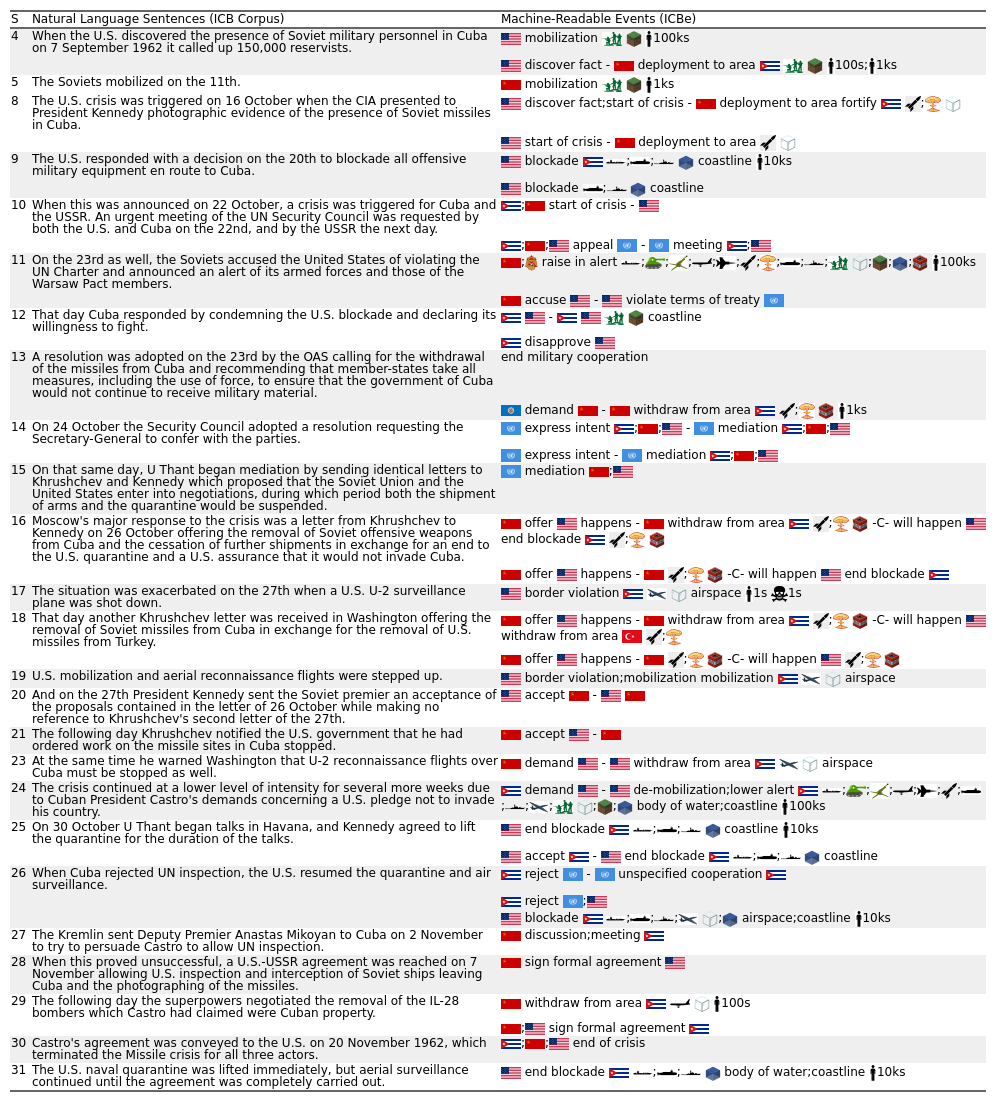
\includegraphics{case_study_cuban_precision.png}
\caption{Cuban Missile Crisis (1962) - ICB Narrative vs.~ICBe
Events}\label{fig-cuba-narrative}
}
\end{figure}

\hypertarget{existing-state-of-the-art-measurements}{%
\subsection{Existing state of the art
measurements}\label{existing-state-of-the-art-measurements}}

We draw informative prior beliefs about the underlying process of
international relations that we expect to govern behavior during
historical episodes and their conversion to the historical record. We
organize our prior beliefs along two overarching axes: existing efforts
to identify the actors/actions of international relations and
identifying a corpus that can be used to produce an ontology of the
information we hope to recover. Table 1 describes these two axes as
columns and rows, respectively.

As we are not the first to attempt to measure international relations in
a structured manner, the columns of Table 1 compare the ontological
coverage of ICBe to existing state of the art systems in production and
with global coverage. We choose these datasets and models as they
represent frequently used and reputable efforts to structure and
describe historical events of interest to scholars of international
politics. The first column starts with our contribution, ICBe, alongside
other event-level datasets including CAMEO dictionary lookup-based
systems (Historical Phoenix
(\textbf{althausClineCenterHistorical2019?}); ICEWS
(\textbf{boscheeICEWSCodedEvent2015?}); Terrier
(\textbf{grantOUEventData2017?})), the Militarized Interstate Disputes
Incidents dataset, and the UCDP-GED dataset
(\textbf{daviesOrganizedViolence19892022?};
\textbf{sundbergIntroducingUCDPGeoreferenced2013?}).\footnote{Other
  related datasets that insufficiently overlap ICBe's domain for
  comparison include BCOW
  (\textbf{lengMilitarizedInterstateCrises1988?}), WEIS
  (\textbf{mcclellandWorldEventInteraction1978?}), CREON
  (\textbf{hermannComparativeResearchEvents1984?}), CASCON
  (\textbf{bloomfieldCASCONIIIComputeraided1989?}), SHERFACS
  (\textbf{shermanSHERFACSCrossParadigmHierarchical2000?}), Real-Time
  Phoenix (\textbf{brandtPhoenixRealTimeEvent2018?}), and COfEE
  (\textbf{balaliCOfEEComprehensiveOntology2021?}) (see histories in
  (\textbf{merrittMeasuringEventsInternational1994?}) and
  (\textbf{schrodtTwentyYearsKansas2006?})).} The final set of columns
compares episode-level datasets beginning with the original ICB project
(\textbf{brecherInternationalCrisisBehavior2021?};
\textbf{brecherCrisesWorldPolitics1982?};
\textbf{beardsleyInternationalCrisisBehavior2020?}); the Militarized
Interstate Disputes dataset (\textbf{palmerMID5Dataset20112021?};
\textbf{giblerInternationalConflicts181620102018?}), and the Correlates
of War (\textbf{sarkeesResortWar181620072010?}). There is imperfect
overlap concerning their intended depth and scope of coverage;
`international crises' are similar, but not identical to, `interstate
wars' and `militarized interstate disputes' which differ yet again from
`individual events of organized violence' and `non-violent action'. Even
like-concepts require care in comparison, as an `aim' in ICBe is the
same as in MIPS, but an `alert' in ICBe is not the same as an `alert' in
MID. Definitions for each ICBe variable are provided in the codebook.

\clearpage
\singlespacing

\global\setlength{\Oldarrayrulewidth}{\arrayrulewidth}

\global\setlength{\Oldtabcolsep}{\tabcolsep}

\setlength{\tabcolsep}{0pt}

\renewcommand*{\arraystretch}{0.75}



\providecommand{\ascline}[3]{\noalign{\global\arrayrulewidth #1}\arrayrulecolor[HTML]{#2}\cline{#3}}

\begin{longtable}[c]{|p{0.10in}|p{2.00in}|p{1.60in}|p{0.22in}|p{0.22in}|p{0.22in}|p{0.22in}|p{0.22in}|p{0.22in}|p{0.22in}|p{0.22in}|p{0.22in}}

\caption{Ontological\ coverage\ of\ ICBe\ versus\ existing\ State\ of\ the\ Art}\\

\hhline{>{\arrayrulecolor[HTML]{000000}\global\arrayrulewidth=2pt}->{\arrayrulecolor[HTML]{000000}\global\arrayrulewidth=2pt}->{\arrayrulecolor[HTML]{000000}\global\arrayrulewidth=2pt}->{\arrayrulecolor[HTML]{000000}\global\arrayrulewidth=2pt}->{\arrayrulecolor[HTML]{000000}\global\arrayrulewidth=2pt}->{\arrayrulecolor[HTML]{000000}\global\arrayrulewidth=2pt}->{\arrayrulecolor[HTML]{000000}\global\arrayrulewidth=2pt}->{\arrayrulecolor[HTML]{000000}\global\arrayrulewidth=2pt}->{\arrayrulecolor[HTML]{000000}\global\arrayrulewidth=2pt}->{\arrayrulecolor[HTML]{000000}\global\arrayrulewidth=2pt}->{\arrayrulecolor[HTML]{000000}\global\arrayrulewidth=2pt}->{\arrayrulecolor[HTML]{000000}\global\arrayrulewidth=2pt}-}

\multicolumn{1}{!{\color[HTML]{000000}\vrule width 2pt}>{\centering}m{\dimexpr 0.1in+0\tabcolsep}}{\rotatebox[origin=c]{270}{\textcolor[HTML]{000000}{\fontsize{6}{6}\selectfont{}}}} & \multicolumn{1}{>{\centering}m{\dimexpr 2in+0\tabcolsep}}{\rotatebox[origin=c]{270}{\textcolor[HTML]{000000}{\fontsize{6}{6}\selectfont{Concept}}}} & \multicolumn{1}{>{\centering}m{\dimexpr 1.6in+0\tabcolsep}}{\rotatebox[origin=c]{270}{\textcolor[HTML]{000000}{\fontsize{6}{6}\selectfont{Literature}}}} & \multicolumn{1}{!{\color[HTML]{666666}\vrule width 1pt}>{\centering}m{\dimexpr 0.22in+0\tabcolsep}}{\rotatebox[origin=c]{270}{\textcolor[HTML]{000000}{\fontsize{6}{6}\selectfont{ICBe}}}} & \multicolumn{1}{>{\centering}m{\dimexpr 0.22in+0\tabcolsep}}{\rotatebox[origin=c]{270}{\textcolor[HTML]{000000}{\fontsize{6}{6}\selectfont{Phoenix}}}} & \multicolumn{1}{>{\centering}m{\dimexpr 0.22in+0\tabcolsep}}{\rotatebox[origin=c]{270}{\textcolor[HTML]{000000}{\fontsize{6}{6}\selectfont{Terrier}}}} & \multicolumn{1}{>{\centering}m{\dimexpr 0.22in+0\tabcolsep}}{\rotatebox[origin=c]{270}{\textcolor[HTML]{000000}{\fontsize{6}{6}\selectfont{ICEWs}}}} & \multicolumn{1}{>{\centering}m{\dimexpr 0.22in+0\tabcolsep}}{\rotatebox[origin=c]{270}{\textcolor[HTML]{000000}{\fontsize{6}{6}\selectfont{MID\ Incidents}}}} & \multicolumn{1}{!{\color[HTML]{666666}\vrule width 1pt}>{\centering}m{\dimexpr 0.22in+0\tabcolsep}}{\rotatebox[origin=c]{270}{\textcolor[HTML]{000000}{\fontsize{6}{6}\selectfont{UCDP-GED}}}} & \multicolumn{1}{>{\centering}m{\dimexpr 0.22in+0\tabcolsep}}{\rotatebox[origin=c]{270}{\textcolor[HTML]{000000}{\fontsize{6}{6}\selectfont{ICB}}}} & \multicolumn{1}{>{\centering}m{\dimexpr 0.22in+0\tabcolsep}}{\rotatebox[origin=c]{270}{\textcolor[HTML]{000000}{\fontsize{6}{6}\selectfont{MIDs}}}} & \multicolumn{1}{>{\centering}m{\dimexpr 0.22in+0\tabcolsep}!{\color[HTML]{000000}\vrule width 2pt}}{\rotatebox[origin=c]{270}{\textcolor[HTML]{000000}{\fontsize{6}{6}\selectfont{COW}}}} \\

\noalign{\global\arrayrulewidth 2pt}\arrayrulecolor[HTML]{000000}

\hhline{|>{\arrayrulecolor[HTML]{000000}\global\arrayrulewidth=2pt}->{\arrayrulecolor[HTML]{000000}\global\arrayrulewidth=2pt}->{\arrayrulecolor[HTML]{000000}\global\arrayrulewidth=2pt}-|>{\arrayrulecolor[HTML]{000000}\global\arrayrulewidth=2pt}->{\arrayrulecolor[HTML]{000000}\global\arrayrulewidth=2pt}->{\arrayrulecolor[HTML]{000000}\global\arrayrulewidth=2pt}->{\arrayrulecolor[HTML]{000000}\global\arrayrulewidth=2pt}->{\arrayrulecolor[HTML]{000000}\global\arrayrulewidth=2pt}-|>{\arrayrulecolor[HTML]{000000}\global\arrayrulewidth=2pt}->{\arrayrulecolor[HTML]{000000}\global\arrayrulewidth=2pt}->{\arrayrulecolor[HTML]{000000}\global\arrayrulewidth=2pt}->{\arrayrulecolor[HTML]{000000}\global\arrayrulewidth=2pt}-}\endfirsthead \caption[]{Ontological\ coverage\ of\ ICBe\ versus\ existing\ State\ of\ the\ Art}\\

\hhline{>{\arrayrulecolor[HTML]{000000}\global\arrayrulewidth=2pt}->{\arrayrulecolor[HTML]{000000}\global\arrayrulewidth=2pt}->{\arrayrulecolor[HTML]{000000}\global\arrayrulewidth=2pt}->{\arrayrulecolor[HTML]{000000}\global\arrayrulewidth=2pt}->{\arrayrulecolor[HTML]{000000}\global\arrayrulewidth=2pt}->{\arrayrulecolor[HTML]{000000}\global\arrayrulewidth=2pt}->{\arrayrulecolor[HTML]{000000}\global\arrayrulewidth=2pt}->{\arrayrulecolor[HTML]{000000}\global\arrayrulewidth=2pt}->{\arrayrulecolor[HTML]{000000}\global\arrayrulewidth=2pt}->{\arrayrulecolor[HTML]{000000}\global\arrayrulewidth=2pt}->{\arrayrulecolor[HTML]{000000}\global\arrayrulewidth=2pt}->{\arrayrulecolor[HTML]{000000}\global\arrayrulewidth=2pt}-}

\multicolumn{1}{!{\color[HTML]{000000}\vrule width 2pt}>{\centering}m{\dimexpr 0.1in+0\tabcolsep}}{\rotatebox[origin=c]{270}{\textcolor[HTML]{000000}{\fontsize{6}{6}\selectfont{}}}} & \multicolumn{1}{>{\centering}m{\dimexpr 2in+0\tabcolsep}}{\rotatebox[origin=c]{270}{\textcolor[HTML]{000000}{\fontsize{6}{6}\selectfont{Concept}}}} & \multicolumn{1}{>{\centering}m{\dimexpr 1.6in+0\tabcolsep}}{\rotatebox[origin=c]{270}{\textcolor[HTML]{000000}{\fontsize{6}{6}\selectfont{Literature}}}} & \multicolumn{1}{!{\color[HTML]{666666}\vrule width 1pt}>{\centering}m{\dimexpr 0.22in+0\tabcolsep}}{\rotatebox[origin=c]{270}{\textcolor[HTML]{000000}{\fontsize{6}{6}\selectfont{ICBe}}}} & \multicolumn{1}{>{\centering}m{\dimexpr 0.22in+0\tabcolsep}}{\rotatebox[origin=c]{270}{\textcolor[HTML]{000000}{\fontsize{6}{6}\selectfont{Phoenix}}}} & \multicolumn{1}{>{\centering}m{\dimexpr 0.22in+0\tabcolsep}}{\rotatebox[origin=c]{270}{\textcolor[HTML]{000000}{\fontsize{6}{6}\selectfont{Terrier}}}} & \multicolumn{1}{>{\centering}m{\dimexpr 0.22in+0\tabcolsep}}{\rotatebox[origin=c]{270}{\textcolor[HTML]{000000}{\fontsize{6}{6}\selectfont{ICEWs}}}} & \multicolumn{1}{>{\centering}m{\dimexpr 0.22in+0\tabcolsep}}{\rotatebox[origin=c]{270}{\textcolor[HTML]{000000}{\fontsize{6}{6}\selectfont{MID\ Incidents}}}} & \multicolumn{1}{!{\color[HTML]{666666}\vrule width 1pt}>{\centering}m{\dimexpr 0.22in+0\tabcolsep}}{\rotatebox[origin=c]{270}{\textcolor[HTML]{000000}{\fontsize{6}{6}\selectfont{UCDP-GED}}}} & \multicolumn{1}{>{\centering}m{\dimexpr 0.22in+0\tabcolsep}}{\rotatebox[origin=c]{270}{\textcolor[HTML]{000000}{\fontsize{6}{6}\selectfont{ICB}}}} & \multicolumn{1}{>{\centering}m{\dimexpr 0.22in+0\tabcolsep}}{\rotatebox[origin=c]{270}{\textcolor[HTML]{000000}{\fontsize{6}{6}\selectfont{MIDs}}}} & \multicolumn{1}{>{\centering}m{\dimexpr 0.22in+0\tabcolsep}!{\color[HTML]{000000}\vrule width 2pt}}{\rotatebox[origin=c]{270}{\textcolor[HTML]{000000}{\fontsize{6}{6}\selectfont{COW}}}} \\

\noalign{\global\arrayrulewidth 2pt}\arrayrulecolor[HTML]{000000}

\hhline{|>{\arrayrulecolor[HTML]{000000}\global\arrayrulewidth=2pt}->{\arrayrulecolor[HTML]{000000}\global\arrayrulewidth=2pt}->{\arrayrulecolor[HTML]{000000}\global\arrayrulewidth=2pt}-|>{\arrayrulecolor[HTML]{000000}\global\arrayrulewidth=2pt}->{\arrayrulecolor[HTML]{000000}\global\arrayrulewidth=2pt}->{\arrayrulecolor[HTML]{000000}\global\arrayrulewidth=2pt}->{\arrayrulecolor[HTML]{000000}\global\arrayrulewidth=2pt}->{\arrayrulecolor[HTML]{000000}\global\arrayrulewidth=2pt}-|>{\arrayrulecolor[HTML]{000000}\global\arrayrulewidth=2pt}->{\arrayrulecolor[HTML]{000000}\global\arrayrulewidth=2pt}->{\arrayrulecolor[HTML]{000000}\global\arrayrulewidth=2pt}->{\arrayrulecolor[HTML]{000000}\global\arrayrulewidth=2pt}-}\endhead



\multicolumn{1}{!{\color[HTML]{000000}\vrule width 2pt}>{\centering}m{\dimexpr 0.1in+0\tabcolsep}}{} & \multicolumn{1}{!{\color[HTML]{666666}\vrule width 1pt}>{\cellcolor[HTML]{EFEFEF}\centering}m{\dimexpr 2in+0\tabcolsep}}{\textcolor[HTML]{000000}{\fontsize{6}{3}\selectfont{Type\ (Episode\ or\ Event)}}} & \multicolumn{1}{>{\cellcolor[HTML]{EFEFEF}\centering}m{\dimexpr 1.6in+0\tabcolsep}}{\textcolor[HTML]{000000}{\fontsize{6}{3}\selectfont{}}} & \multicolumn{1}{!{\color[HTML]{666666}\vrule width 1pt}>{\cellcolor[HTML]{EFEFEF}\centering}m{\dimexpr 0.22in+0\tabcolsep}}{\textcolor[HTML]{000000}{\fontsize{6}{3}\selectfont{Ep}}} & \multicolumn{1}{>{\cellcolor[HTML]{EFEFEF}\centering}m{\dimexpr 0.22in+0\tabcolsep}}{\textcolor[HTML]{000000}{\fontsize{6}{3}\selectfont{Ep}}} & \multicolumn{1}{>{\cellcolor[HTML]{EFEFEF}\centering}m{\dimexpr 0.22in+0\tabcolsep}}{\textcolor[HTML]{000000}{\fontsize{6}{3}\selectfont{Ep}}} & \multicolumn{1}{>{\cellcolor[HTML]{EFEFEF}\centering}m{\dimexpr 0.22in+0\tabcolsep}}{\textcolor[HTML]{000000}{\fontsize{6}{3}\selectfont{Ep}}} & \multicolumn{1}{>{\cellcolor[HTML]{EFEFEF}\centering}m{\dimexpr 0.22in+0\tabcolsep}}{\textcolor[HTML]{000000}{\fontsize{6}{3}\selectfont{Ep}}} & \multicolumn{1}{!{\color[HTML]{666666}\vrule width 1pt}>{\cellcolor[HTML]{EFEFEF}\centering}m{\dimexpr 0.22in+0\tabcolsep}}{\textcolor[HTML]{000000}{\fontsize{6}{3}\selectfont{Ev}}} & \multicolumn{1}{>{\cellcolor[HTML]{EFEFEF}\centering}m{\dimexpr 0.22in+0\tabcolsep}}{\textcolor[HTML]{000000}{\fontsize{6}{3}\selectfont{Ev}}} & \multicolumn{1}{>{\cellcolor[HTML]{EFEFEF}\centering}m{\dimexpr 0.22in+0\tabcolsep}}{\textcolor[HTML]{000000}{\fontsize{6}{3}\selectfont{Ev}}} & \multicolumn{1}{>{\cellcolor[HTML]{EFEFEF}\centering}m{\dimexpr 0.22in+0\tabcolsep}!{\color[HTML]{000000}\vrule width 2pt}}{\textcolor[HTML]{000000}{\fontsize{6}{3}\selectfont{Ev}}} \\

\noalign{\global\arrayrulewidth 2pt}\arrayrulecolor[HTML]{000000}

\hhline{>{\arrayrulecolor[HTML]{FFFFFF}\global\arrayrulewidth=0pt}-~~|~~~~~|~~~~}



\multicolumn{1}{!{\color[HTML]{000000}\vrule width 2pt}>{\centering}m{\dimexpr 0.1in+0\tabcolsep}}{} & \multicolumn{1}{!{\color[HTML]{666666}\vrule width 1pt}>{\centering}m{\dimexpr 2in+0\tabcolsep}}{\textcolor[HTML]{000000}{\fontsize{6}{3}\selectfont{Start}}} & \multicolumn{1}{>{\centering}m{\dimexpr 1.6in+0\tabcolsep}}{\textcolor[HTML]{000000}{\fontsize{6}{3}\selectfont{}}} & \multicolumn{1}{!{\color[HTML]{666666}\vrule width 1pt}>{\centering}m{\dimexpr 0.22in+0\tabcolsep}}{\textcolor[HTML]{000000}{\fontsize{6}{3}\selectfont{1918}}} & \multicolumn{1}{>{\centering}m{\dimexpr 0.22in+0\tabcolsep}}{\textcolor[HTML]{000000}{\fontsize{6}{3}\selectfont{1945}}} & \multicolumn{1}{>{\centering}m{\dimexpr 0.22in+0\tabcolsep}}{\textcolor[HTML]{000000}{\fontsize{6}{3}\selectfont{1977}}} & \multicolumn{1}{>{\centering}m{\dimexpr 0.22in+0\tabcolsep}}{\textcolor[HTML]{000000}{\fontsize{6}{3}\selectfont{1995}}} & \multicolumn{1}{>{\centering}m{\dimexpr 0.22in+0\tabcolsep}}{\textcolor[HTML]{000000}{\fontsize{6}{3}\selectfont{1993}}} & \multicolumn{1}{!{\color[HTML]{666666}\vrule width 1pt}>{\centering}m{\dimexpr 0.22in+0\tabcolsep}}{\textcolor[HTML]{000000}{\fontsize{6}{3}\selectfont{1989}}} & \multicolumn{1}{>{\centering}m{\dimexpr 0.22in+0\tabcolsep}}{\textcolor[HTML]{000000}{\fontsize{6}{3}\selectfont{1918}}} & \multicolumn{1}{>{\centering}m{\dimexpr 0.22in+0\tabcolsep}}{\textcolor[HTML]{000000}{\fontsize{6}{3}\selectfont{1816}}} & \multicolumn{1}{>{\centering}m{\dimexpr 0.22in+0\tabcolsep}!{\color[HTML]{000000}\vrule width 2pt}}{\textcolor[HTML]{000000}{\fontsize{6}{3}\selectfont{1816}}} \\

\noalign{\global\arrayrulewidth 2pt}\arrayrulecolor[HTML]{000000}

\hhline{>{\arrayrulecolor[HTML]{FFFFFF}\global\arrayrulewidth=0pt}-~~|~~~~~|~~~~}



\multicolumn{1}{!{\color[HTML]{000000}\vrule width 2pt}>{\centering}m{\dimexpr 0.1in+0\tabcolsep}}{} & \multicolumn{1}{!{\color[HTML]{666666}\vrule width 1pt}>{\cellcolor[HTML]{EFEFEF}\centering}m{\dimexpr 2in+0\tabcolsep}}{\textcolor[HTML]{000000}{\fontsize{6}{3}\selectfont{End}}} & \multicolumn{1}{>{\cellcolor[HTML]{EFEFEF}\centering}m{\dimexpr 1.6in+0\tabcolsep}}{\textcolor[HTML]{000000}{\fontsize{6}{3}\selectfont{}}} & \multicolumn{1}{!{\color[HTML]{666666}\vrule width 1pt}>{\cellcolor[HTML]{EFEFEF}\centering}m{\dimexpr 0.22in+0\tabcolsep}}{\textcolor[HTML]{000000}{\fontsize{6}{3}\selectfont{2017}}} & \multicolumn{1}{>{\cellcolor[HTML]{EFEFEF}\centering}m{\dimexpr 0.22in+0\tabcolsep}}{\textcolor[HTML]{000000}{\fontsize{6}{3}\selectfont{2019}}} & \multicolumn{1}{>{\cellcolor[HTML]{EFEFEF}\centering}m{\dimexpr 0.22in+0\tabcolsep}}{\textcolor[HTML]{000000}{\fontsize{6}{3}\selectfont{2018}}} & \multicolumn{1}{>{\cellcolor[HTML]{EFEFEF}\centering}m{\dimexpr 0.22in+0\tabcolsep}}{\textcolor[HTML]{000000}{\fontsize{6}{3}\selectfont{2020}}} & \multicolumn{1}{>{\cellcolor[HTML]{EFEFEF}\centering}m{\dimexpr 0.22in+0\tabcolsep}}{\textcolor[HTML]{000000}{\fontsize{6}{3}\selectfont{2010}}} & \multicolumn{1}{!{\color[HTML]{666666}\vrule width 1pt}>{\cellcolor[HTML]{EFEFEF}\centering}m{\dimexpr 0.22in+0\tabcolsep}}{\textcolor[HTML]{000000}{\fontsize{6}{3}\selectfont{2015}}} & \multicolumn{1}{>{\cellcolor[HTML]{EFEFEF}\centering}m{\dimexpr 0.22in+0\tabcolsep}}{\textcolor[HTML]{000000}{\fontsize{6}{3}\selectfont{2017}}} & \multicolumn{1}{>{\cellcolor[HTML]{EFEFEF}\centering}m{\dimexpr 0.22in+0\tabcolsep}}{\textcolor[HTML]{000000}{\fontsize{6}{3}\selectfont{2014}}} & \multicolumn{1}{>{\cellcolor[HTML]{EFEFEF}\centering}m{\dimexpr 0.22in+0\tabcolsep}!{\color[HTML]{000000}\vrule width 2pt}}{\textcolor[HTML]{000000}{\fontsize{6}{3}\selectfont{2007}}} \\

\noalign{\global\arrayrulewidth 2pt}\arrayrulecolor[HTML]{000000}

\hhline{>{\arrayrulecolor[HTML]{FFFFFF}\global\arrayrulewidth=0pt}-~~|~~~~~|~~~~}



\multicolumn{1}{!{\color[HTML]{000000}\vrule width 2pt}>{\centering}m{\dimexpr 0.1in+0\tabcolsep}}{} & \multicolumn{1}{!{\color[HTML]{666666}\vrule width 1pt}>{\centering}m{\dimexpr 2in+0\tabcolsep}}{\textcolor[HTML]{000000}{\fontsize{6}{3}\selectfont{N}}} & \multicolumn{1}{>{\centering}m{\dimexpr 1.6in+0\tabcolsep}}{\textcolor[HTML]{000000}{\fontsize{6}{3}\selectfont{}}} & \multicolumn{1}{!{\color[HTML]{666666}\vrule width 1pt}>{\centering}m{\dimexpr 0.22in+0\tabcolsep}}{\textcolor[HTML]{000000}{\fontsize{6}{3}\selectfont{32K}}} & \multicolumn{1}{>{\centering}m{\dimexpr 0.22in+0\tabcolsep}}{\textcolor[HTML]{000000}{\fontsize{6}{3}\selectfont{8.5M}}} & \multicolumn{1}{>{\centering}m{\dimexpr 0.22in+0\tabcolsep}}{\textcolor[HTML]{000000}{\fontsize{6}{3}\selectfont{28.4M}}} & \multicolumn{1}{>{\centering}m{\dimexpr 0.22in+0\tabcolsep}}{\textcolor[HTML]{000000}{\fontsize{6}{3}\selectfont{17.5M}}} & \multicolumn{1}{>{\centering}m{\dimexpr 0.22in+0\tabcolsep}}{\textcolor[HTML]{000000}{\fontsize{6}{3}\selectfont{9.6K}}} & \multicolumn{1}{!{\color[HTML]{666666}\vrule width 1pt}>{\centering}m{\dimexpr 0.22in+0\tabcolsep}}{\textcolor[HTML]{000000}{\fontsize{6}{3}\selectfont{128K}}} & \multicolumn{1}{>{\centering}m{\dimexpr 0.22in+0\tabcolsep}}{\textcolor[HTML]{000000}{\fontsize{6}{3}\selectfont{1K}}} & \multicolumn{1}{>{\centering}m{\dimexpr 0.22in+0\tabcolsep}}{\textcolor[HTML]{000000}{\fontsize{6}{3}\selectfont{5.9K}}} & \multicolumn{1}{>{\centering}m{\dimexpr 0.22in+0\tabcolsep}!{\color[HTML]{000000}\vrule width 2pt}}{\textcolor[HTML]{000000}{\fontsize{6}{3}\selectfont{1K}}} \\

\noalign{\global\arrayrulewidth 2pt}\arrayrulecolor[HTML]{000000}

\hhline{>{\arrayrulecolor[HTML]{FFFFFF}\global\arrayrulewidth=0pt}-~~|~~~~~|~~~~}



\multicolumn{1}{!{\color[HTML]{000000}\vrule width 2pt}>{\centering}m{\dimexpr 0.1in+0\tabcolsep}}{} & \multicolumn{1}{!{\color[HTML]{666666}\vrule width 1pt}>{\cellcolor[HTML]{EFEFEF}\centering}m{\dimexpr 2in+0\tabcolsep}}{\textcolor[HTML]{000000}{\fontsize{6}{3}\selectfont{Coders\ (Hand\ or\ Automated)}}} & \multicolumn{1}{>{\cellcolor[HTML]{EFEFEF}\centering}m{\dimexpr 1.6in+0\tabcolsep}}{\textcolor[HTML]{000000}{\fontsize{6}{3}\selectfont{}}} & \multicolumn{1}{!{\color[HTML]{666666}\vrule width 1pt}>{\cellcolor[HTML]{EFEFEF}\centering}m{\dimexpr 0.22in+0\tabcolsep}}{\textcolor[HTML]{000000}{\fontsize{6}{3}\selectfont{H}}} & \multicolumn{1}{>{\cellcolor[HTML]{EFEFEF}\centering}m{\dimexpr 0.22in+0\tabcolsep}}{\textcolor[HTML]{000000}{\fontsize{6}{3}\selectfont{A}}} & \multicolumn{1}{>{\cellcolor[HTML]{EFEFEF}\centering}m{\dimexpr 0.22in+0\tabcolsep}}{\textcolor[HTML]{000000}{\fontsize{6}{3}\selectfont{A}}} & \multicolumn{1}{>{\cellcolor[HTML]{EFEFEF}\centering}m{\dimexpr 0.22in+0\tabcolsep}}{\textcolor[HTML]{000000}{\fontsize{6}{3}\selectfont{A}}} & \multicolumn{1}{>{\cellcolor[HTML]{EFEFEF}\centering}m{\dimexpr 0.22in+0\tabcolsep}}{\textcolor[HTML]{000000}{\fontsize{6}{3}\selectfont{H}}} & \multicolumn{1}{!{\color[HTML]{666666}\vrule width 1pt}>{\cellcolor[HTML]{EFEFEF}\centering}m{\dimexpr 0.22in+0\tabcolsep}}{\textcolor[HTML]{000000}{\fontsize{6}{3}\selectfont{H}}} & \multicolumn{1}{>{\cellcolor[HTML]{EFEFEF}\centering}m{\dimexpr 0.22in+0\tabcolsep}}{\textcolor[HTML]{000000}{\fontsize{6}{3}\selectfont{H}}} & \multicolumn{1}{>{\cellcolor[HTML]{EFEFEF}\centering}m{\dimexpr 0.22in+0\tabcolsep}}{\textcolor[HTML]{000000}{\fontsize{6}{3}\selectfont{H}}} & \multicolumn{1}{>{\cellcolor[HTML]{EFEFEF}\centering}m{\dimexpr 0.22in+0\tabcolsep}!{\color[HTML]{000000}\vrule width 2pt}}{\textcolor[HTML]{000000}{\fontsize{6}{3}\selectfont{H}}} \\

\noalign{\global\arrayrulewidth 2pt}\arrayrulecolor[HTML]{000000}

\hhline{>{\arrayrulecolor[HTML]{FFFFFF}\global\arrayrulewidth=0pt}-~~|~~~~~|~~~~}



\multicolumn{1}{!{\color[HTML]{000000}\vrule width 2pt}>{\centering}m{\dimexpr 0.1in+0\tabcolsep}}{} & \multicolumn{1}{!{\color[HTML]{666666}\vrule width 1pt}>{\centering}m{\dimexpr 2in+0\tabcolsep}}{\textcolor[HTML]{000000}{\fontsize{6}{3}\selectfont{Corpus}}} & \multicolumn{1}{>{\centering}m{\dimexpr 1.6in+0\tabcolsep}}{\textcolor[HTML]{000000}{\fontsize{6}{3}\selectfont{}}} & \multicolumn{1}{!{\color[HTML]{666666}\vrule width 1pt}>{\centering}m{\dimexpr 0.22in+0\tabcolsep}}{\textcolor[HTML]{000000}{\fontsize{6}{3}\selectfont{ICB}}} & \multicolumn{1}{>{\centering}m{\dimexpr 0.22in+0\tabcolsep}}{\textcolor[HTML]{000000}{\fontsize{6}{3}\selectfont{News}}} & \multicolumn{1}{>{\centering}m{\dimexpr 0.22in+0\tabcolsep}}{\textcolor[HTML]{000000}{\fontsize{6}{3}\selectfont{News}}} & \multicolumn{1}{>{\centering}m{\dimexpr 0.22in+0\tabcolsep}}{\textcolor[HTML]{000000}{\fontsize{6}{3}\selectfont{News}}} & \multicolumn{1}{>{\centering}m{\dimexpr 0.22in+0\tabcolsep}}{\textcolor[HTML]{000000}{\fontsize{6}{3}\selectfont{Mix}}} & \multicolumn{1}{!{\color[HTML]{666666}\vrule width 1pt}>{\centering}m{\dimexpr 0.22in+0\tabcolsep}}{\textcolor[HTML]{000000}{\fontsize{6}{3}\selectfont{News}}} & \multicolumn{1}{>{\centering}m{\dimexpr 0.22in+0\tabcolsep}}{\textcolor[HTML]{000000}{\fontsize{6}{3}\selectfont{Mix}}} & \multicolumn{1}{>{\centering}m{\dimexpr 0.22in+0\tabcolsep}}{\textcolor[HTML]{000000}{\fontsize{6}{3}\selectfont{Mix}}} & \multicolumn{1}{>{\centering}m{\dimexpr 0.22in+0\tabcolsep}!{\color[HTML]{000000}\vrule width 2pt}}{\textcolor[HTML]{000000}{\fontsize{6}{3}\selectfont{Mix}}} \\

\noalign{\global\arrayrulewidth 2pt}\arrayrulecolor[HTML]{000000}

\hhline{>{\arrayrulecolor[HTML]{FFFFFF}\global\arrayrulewidth=0pt}-~~|~~~~~|~~~~}



\multicolumn{1}{!{\color[HTML]{000000}\vrule width 2pt}>{\centering}m{\dimexpr 0.1in+0\tabcolsep}}{} & \multicolumn{1}{!{\color[HTML]{666666}\vrule width 1pt}>{\cellcolor[HTML]{EFEFEF}\centering}m{\dimexpr 2in+0\tabcolsep}}{\textcolor[HTML]{000000}{\fontsize{6}{3}\selectfont{Date\ source\ (Event\ or\ Article)}}} & \multicolumn{1}{>{\cellcolor[HTML]{EFEFEF}\centering}m{\dimexpr 1.6in+0\tabcolsep}}{\textcolor[HTML]{000000}{\fontsize{6}{3}\selectfont{}}} & \multicolumn{1}{!{\color[HTML]{666666}\vrule width 1pt}>{\cellcolor[HTML]{EFEFEF}\centering}m{\dimexpr 0.22in+0\tabcolsep}}{\textcolor[HTML]{000000}{\fontsize{6}{3}\selectfont{E}}} & \multicolumn{1}{>{\cellcolor[HTML]{EFEFEF}\centering}m{\dimexpr 0.22in+0\tabcolsep}}{\textcolor[HTML]{000000}{\fontsize{6}{3}\selectfont{A}}} & \multicolumn{1}{>{\cellcolor[HTML]{EFEFEF}\centering}m{\dimexpr 0.22in+0\tabcolsep}}{\textcolor[HTML]{000000}{\fontsize{6}{3}\selectfont{A}}} & \multicolumn{1}{>{\cellcolor[HTML]{EFEFEF}\centering}m{\dimexpr 0.22in+0\tabcolsep}}{\textcolor[HTML]{000000}{\fontsize{6}{3}\selectfont{A}}} & \multicolumn{1}{>{\cellcolor[HTML]{EFEFEF}\centering}m{\dimexpr 0.22in+0\tabcolsep}}{\textcolor[HTML]{000000}{\fontsize{6}{3}\selectfont{E}}} & \multicolumn{1}{!{\color[HTML]{666666}\vrule width 1pt}>{\cellcolor[HTML]{EFEFEF}\centering}m{\dimexpr 0.22in+0\tabcolsep}}{\textcolor[HTML]{000000}{\fontsize{6}{3}\selectfont{A}}} & \multicolumn{1}{>{\cellcolor[HTML]{EFEFEF}\centering}m{\dimexpr 0.22in+0\tabcolsep}}{\textcolor[HTML]{000000}{\fontsize{6}{3}\selectfont{E}}} & \multicolumn{1}{>{\cellcolor[HTML]{EFEFEF}\centering}m{\dimexpr 0.22in+0\tabcolsep}}{\textcolor[HTML]{000000}{\fontsize{6}{3}\selectfont{E}}} & \multicolumn{1}{>{\cellcolor[HTML]{EFEFEF}\centering}m{\dimexpr 0.22in+0\tabcolsep}!{\color[HTML]{000000}\vrule width 2pt}}{\textcolor[HTML]{000000}{\fontsize{6}{3}\selectfont{E}}} \\

\noalign{\global\arrayrulewidth 2pt}\arrayrulecolor[HTML]{000000}

\hhline{>{\arrayrulecolor[HTML]{FFFFFF}\global\arrayrulewidth=0pt}-~~|~~~~~|~~~~}



\multicolumn{1}{!{\color[HTML]{000000}\vrule width 2pt}>{\centering}m{\dimexpr 0.1in+0\tabcolsep}}{\multirow[c]{-8}{*}{\parbox{0.1in}{\centering \rotatebox[origin=c]{270}{\textcolor[HTML]{000000}{\fontsize{6}{3}\selectfont{Domain}}}}}} & \multicolumn{1}{!{\color[HTML]{666666}\vrule width 1pt}>{\centering}m{\dimexpr 2in+0\tabcolsep}}{\textcolor[HTML]{000000}{\fontsize{6}{3}\selectfont{Location\ source\ (Event\ or\ Actor)}}} & \multicolumn{1}{>{\centering}m{\dimexpr 1.6in+0\tabcolsep}}{\textcolor[HTML]{000000}{\fontsize{6}{3}\selectfont{}}} & \multicolumn{1}{!{\color[HTML]{666666}\vrule width 1pt}>{\centering}m{\dimexpr 0.22in+0\tabcolsep}}{\textcolor[HTML]{000000}{\fontsize{6}{3}\selectfont{E}}} & \multicolumn{1}{>{\centering}m{\dimexpr 0.22in+0\tabcolsep}}{\textcolor[HTML]{000000}{\fontsize{6}{3}\selectfont{E}}} & \multicolumn{1}{>{\centering}m{\dimexpr 0.22in+0\tabcolsep}}{\textcolor[HTML]{000000}{\fontsize{6}{3}\selectfont{E}}} & \multicolumn{1}{>{\centering}m{\dimexpr 0.22in+0\tabcolsep}}{\textcolor[HTML]{000000}{\fontsize{6}{3}\selectfont{E}}} & \multicolumn{1}{>{\centering}m{\dimexpr 0.22in+0\tabcolsep}}{\textcolor[HTML]{000000}{\fontsize{6}{3}\selectfont{A}}} & \multicolumn{1}{!{\color[HTML]{666666}\vrule width 1pt}>{\centering}m{\dimexpr 0.22in+0\tabcolsep}}{\textcolor[HTML]{000000}{\fontsize{6}{3}\selectfont{E}}} & \multicolumn{1}{>{\centering}m{\dimexpr 0.22in+0\tabcolsep}}{\textcolor[HTML]{000000}{\fontsize{6}{3}\selectfont{A}}} & \multicolumn{1}{>{\centering}m{\dimexpr 0.22in+0\tabcolsep}}{\textcolor[HTML]{000000}{\fontsize{6}{3}\selectfont{E}}} & \multicolumn{1}{>{\centering}m{\dimexpr 0.22in+0\tabcolsep}!{\color[HTML]{000000}\vrule width 2pt}}{\textcolor[HTML]{000000}{\fontsize{6}{3}\selectfont{A}}} \\

\noalign{\global\arrayrulewidth 2pt}\arrayrulecolor[HTML]{000000}

\hhline{|>{\arrayrulecolor[HTML]{666666}\global\arrayrulewidth=1pt}-|>{\arrayrulecolor[HTML]{666666}\global\arrayrulewidth=1pt}->{\arrayrulecolor[HTML]{666666}\global\arrayrulewidth=1pt}-|>{\arrayrulecolor[HTML]{666666}\global\arrayrulewidth=1pt}->{\arrayrulecolor[HTML]{666666}\global\arrayrulewidth=1pt}->{\arrayrulecolor[HTML]{666666}\global\arrayrulewidth=1pt}->{\arrayrulecolor[HTML]{666666}\global\arrayrulewidth=1pt}->{\arrayrulecolor[HTML]{666666}\global\arrayrulewidth=1pt}-|>{\arrayrulecolor[HTML]{666666}\global\arrayrulewidth=1pt}->{\arrayrulecolor[HTML]{666666}\global\arrayrulewidth=1pt}->{\arrayrulecolor[HTML]{666666}\global\arrayrulewidth=1pt}->{\arrayrulecolor[HTML]{666666}\global\arrayrulewidth=1pt}-}



\multicolumn{1}{!{\color[HTML]{000000}\vrule width 2pt}>{\centering}m{\dimexpr 0.1in+0\tabcolsep}}{} & \multicolumn{1}{!{\color[HTML]{666666}\vrule width 1pt}>{\cellcolor[HTML]{EFEFEF}\centering}m{\dimexpr 2in+0\tabcolsep}}{\textcolor[HTML]{000000}{\fontsize{6}{3}\selectfont{States}}} & \multicolumn{1}{>{\cellcolor[HTML]{EFEFEF}\centering}m{\dimexpr 1.6in+0\tabcolsep}}{\textcolor[HTML]{000000}{\fontsize{6}{3}\selectfont{(}}\textcolor[HTML]{000000}{\fontsize{6}{3}\selectfont{\textbf{fazalStateDeathPolitics2011?}}}\textcolor[HTML]{000000}{\fontsize{6}{3}\selectfont{)}}\textcolor[HTML]{000000}{\fontsize{6}{3}\selectfont{,}}\textcolor[HTML]{000000}{\fontsize{6}{3}\selectfont{\ }}\textcolor[HTML]{000000}{\fontsize{6}{3}\selectfont{(}}\textcolor[HTML]{000000}{\fontsize{6}{3}\selectfont{\textbf{spruytSovereignStateIts1996?}}}\textcolor[HTML]{000000}{\fontsize{6}{3}\selectfont{)}}} & \multicolumn{1}{!{\color[HTML]{666666}\vrule width 1pt}>{\cellcolor[HTML]{EFEFEF}\centering}m{\dimexpr 0.22in+0\tabcolsep}}{\textcolor[HTML]{000000}{\fontsize{6}{3}\selectfont{✓}}} & \multicolumn{1}{>{\cellcolor[HTML]{EFEFEF}\centering}m{\dimexpr 0.22in+0\tabcolsep}}{\textcolor[HTML]{000000}{\fontsize{6}{3}\selectfont{✓}}} & \multicolumn{1}{>{\cellcolor[HTML]{EFEFEF}\centering}m{\dimexpr 0.22in+0\tabcolsep}}{\textcolor[HTML]{000000}{\fontsize{6}{3}\selectfont{✓}}} & \multicolumn{1}{>{\cellcolor[HTML]{EFEFEF}\centering}m{\dimexpr 0.22in+0\tabcolsep}}{\textcolor[HTML]{000000}{\fontsize{6}{3}\selectfont{✓}}} & \multicolumn{1}{>{\cellcolor[HTML]{EFEFEF}\centering}m{\dimexpr 0.22in+0\tabcolsep}}{\textcolor[HTML]{000000}{\fontsize{6}{3}\selectfont{✓}}} & \multicolumn{1}{!{\color[HTML]{666666}\vrule width 1pt}>{\cellcolor[HTML]{EFEFEF}\centering}m{\dimexpr 0.22in+0\tabcolsep}}{\textcolor[HTML]{000000}{\fontsize{6}{3}\selectfont{✓}}} & \multicolumn{1}{>{\cellcolor[HTML]{EFEFEF}\centering}m{\dimexpr 0.22in+0\tabcolsep}}{\textcolor[HTML]{000000}{\fontsize{6}{3}\selectfont{✓}}} & \multicolumn{1}{>{\cellcolor[HTML]{EFEFEF}\centering}m{\dimexpr 0.22in+0\tabcolsep}}{\textcolor[HTML]{000000}{\fontsize{6}{3}\selectfont{✓}}} & \multicolumn{1}{>{\cellcolor[HTML]{EFEFEF}\centering}m{\dimexpr 0.22in+0\tabcolsep}!{\color[HTML]{000000}\vrule width 2pt}}{\textcolor[HTML]{000000}{\fontsize{6}{3}\selectfont{✓}}} \\

\noalign{\global\arrayrulewidth 2pt}\arrayrulecolor[HTML]{000000}

\hhline{>{\arrayrulecolor[HTML]{FFFFFF}\global\arrayrulewidth=0pt}-~~|~~~~~|~~~~}



\multicolumn{1}{!{\color[HTML]{000000}\vrule width 2pt}>{\centering}m{\dimexpr 0.1in+0\tabcolsep}}{} & \multicolumn{1}{!{\color[HTML]{666666}\vrule width 1pt}>{\centering}m{\dimexpr 2in+0\tabcolsep}}{\textcolor[HTML]{000000}{\fontsize{6}{3}\selectfont{Subnational\ Actors}}} & \multicolumn{1}{>{\centering}m{\dimexpr 1.6in+0\tabcolsep}}{\textcolor[HTML]{000000}{\fontsize{6}{3}\selectfont{(}}\textcolor[HTML]{000000}{\fontsize{6}{3}\selectfont{\textbf{haffarEmergentPeacemakersCataloguing2002?}}}\textcolor[HTML]{000000}{\fontsize{6}{3}\selectfont{)}}} & \multicolumn{1}{!{\color[HTML]{666666}\vrule width 1pt}>{\centering}m{\dimexpr 0.22in+0\tabcolsep}}{\textcolor[HTML]{000000}{\fontsize{6}{3}\selectfont{✓}}} & \multicolumn{1}{>{\centering}m{\dimexpr 0.22in+0\tabcolsep}}{\textcolor[HTML]{000000}{\fontsize{6}{3}\selectfont{✓}}} & \multicolumn{1}{>{\centering}m{\dimexpr 0.22in+0\tabcolsep}}{\textcolor[HTML]{000000}{\fontsize{6}{3}\selectfont{✓}}} & \multicolumn{1}{>{\centering}m{\dimexpr 0.22in+0\tabcolsep}}{\textcolor[HTML]{000000}{\fontsize{6}{3}\selectfont{✓}}} & \multicolumn{1}{>{\centering}m{\dimexpr 0.22in+0\tabcolsep}}{\textcolor[HTML]{000000}{\fontsize{6}{3}\selectfont{}}} & \multicolumn{1}{!{\color[HTML]{666666}\vrule width 1pt}>{\centering}m{\dimexpr 0.22in+0\tabcolsep}}{\textcolor[HTML]{000000}{\fontsize{6}{3}\selectfont{✓}}} & \multicolumn{1}{>{\centering}m{\dimexpr 0.22in+0\tabcolsep}}{\textcolor[HTML]{000000}{\fontsize{6}{3}\selectfont{}}} & \multicolumn{1}{>{\centering}m{\dimexpr 0.22in+0\tabcolsep}}{\textcolor[HTML]{000000}{\fontsize{6}{3}\selectfont{}}} & \multicolumn{1}{>{\centering}m{\dimexpr 0.22in+0\tabcolsep}!{\color[HTML]{000000}\vrule width 2pt}}{\textcolor[HTML]{000000}{\fontsize{6}{3}\selectfont{✓}}} \\

\noalign{\global\arrayrulewidth 2pt}\arrayrulecolor[HTML]{000000}

\hhline{>{\arrayrulecolor[HTML]{FFFFFF}\global\arrayrulewidth=0pt}-~~|~~~~~|~~~~}



\multicolumn{1}{!{\color[HTML]{000000}\vrule width 2pt}>{\centering}m{\dimexpr 0.1in+0\tabcolsep}}{} & \multicolumn{1}{!{\color[HTML]{666666}\vrule width 1pt}>{\cellcolor[HTML]{EFEFEF}\centering}m{\dimexpr 2in+0\tabcolsep}}{\textcolor[HTML]{000000}{\fontsize{6}{3}\selectfont{IGO/NGO}}} & \multicolumn{1}{>{\cellcolor[HTML]{EFEFEF}\centering}m{\dimexpr 1.6in+0\tabcolsep}}{\textcolor[HTML]{000000}{\fontsize{6}{3}\selectfont{(}}\textcolor[HTML]{000000}{\fontsize{6}{3}\selectfont{\textbf{bushDensityDeclineFounding2019?}}}\textcolor[HTML]{000000}{\fontsize{6}{3}\selectfont{)}}} & \multicolumn{1}{!{\color[HTML]{666666}\vrule width 1pt}>{\cellcolor[HTML]{EFEFEF}\centering}m{\dimexpr 0.22in+0\tabcolsep}}{\textcolor[HTML]{000000}{\fontsize{6}{3}\selectfont{✓}}} & \multicolumn{1}{>{\cellcolor[HTML]{EFEFEF}\centering}m{\dimexpr 0.22in+0\tabcolsep}}{\textcolor[HTML]{000000}{\fontsize{6}{3}\selectfont{✓}}} & \multicolumn{1}{>{\cellcolor[HTML]{EFEFEF}\centering}m{\dimexpr 0.22in+0\tabcolsep}}{\textcolor[HTML]{000000}{\fontsize{6}{3}\selectfont{✓}}} & \multicolumn{1}{>{\cellcolor[HTML]{EFEFEF}\centering}m{\dimexpr 0.22in+0\tabcolsep}}{\textcolor[HTML]{000000}{\fontsize{6}{3}\selectfont{✓}}} & \multicolumn{1}{>{\cellcolor[HTML]{EFEFEF}\centering}m{\dimexpr 0.22in+0\tabcolsep}}{\textcolor[HTML]{000000}{\fontsize{6}{3}\selectfont{}}} & \multicolumn{1}{!{\color[HTML]{666666}\vrule width 1pt}>{\cellcolor[HTML]{EFEFEF}\centering}m{\dimexpr 0.22in+0\tabcolsep}}{\textcolor[HTML]{000000}{\fontsize{6}{3}\selectfont{}}} & \multicolumn{1}{>{\cellcolor[HTML]{EFEFEF}\centering}m{\dimexpr 0.22in+0\tabcolsep}}{\textcolor[HTML]{000000}{\fontsize{6}{3}\selectfont{✓}}} & \multicolumn{1}{>{\cellcolor[HTML]{EFEFEF}\centering}m{\dimexpr 0.22in+0\tabcolsep}}{\textcolor[HTML]{000000}{\fontsize{6}{3}\selectfont{}}} & \multicolumn{1}{>{\cellcolor[HTML]{EFEFEF}\centering}m{\dimexpr 0.22in+0\tabcolsep}!{\color[HTML]{000000}\vrule width 2pt}}{\textcolor[HTML]{000000}{\fontsize{6}{3}\selectfont{}}} \\

\noalign{\global\arrayrulewidth 2pt}\arrayrulecolor[HTML]{000000}

\hhline{>{\arrayrulecolor[HTML]{FFFFFF}\global\arrayrulewidth=0pt}-~~|~~~~~|~~~~}



\multicolumn{1}{!{\color[HTML]{000000}\vrule width 2pt}>{\centering}m{\dimexpr 0.1in+0\tabcolsep}}{\multirow[c]{-4}{*}{\parbox{0.1in}{\centering \rotatebox[origin=c]{270}{\textcolor[HTML]{000000}{\fontsize{6}{3}\selectfont{Players}}}}}} & \multicolumn{1}{!{\color[HTML]{666666}\vrule width 1pt}>{\centering}m{\dimexpr 2in+0\tabcolsep}}{\textcolor[HTML]{000000}{\fontsize{6}{3}\selectfont{Civilians}}} & \multicolumn{1}{>{\centering}m{\dimexpr 1.6in+0\tabcolsep}}{\textcolor[HTML]{000000}{\fontsize{6}{3}\selectfont{Ben-Yehuda}}\textcolor[HTML]{000000}{\fontsize{6}{3}\selectfont{\ }}\textcolor[HTML]{000000}{\fontsize{6}{3}\selectfont{and}}\textcolor[HTML]{000000}{\fontsize{6}{3}\selectfont{\ }}\textcolor[HTML]{000000}{\fontsize{6}{3}\selectfont{Mishali–Ram}}\textcolor[HTML]{000000}{\fontsize{6}{3}\selectfont{\ }}\textcolor[HTML]{000000}{\fontsize{6}{3}\selectfont{(2006)}}} & \multicolumn{1}{!{\color[HTML]{666666}\vrule width 1pt}>{\centering}m{\dimexpr 0.22in+0\tabcolsep}}{\textcolor[HTML]{000000}{\fontsize{6}{3}\selectfont{✓}}} & \multicolumn{1}{>{\centering}m{\dimexpr 0.22in+0\tabcolsep}}{\textcolor[HTML]{000000}{\fontsize{6}{3}\selectfont{✓}}} & \multicolumn{1}{>{\centering}m{\dimexpr 0.22in+0\tabcolsep}}{\textcolor[HTML]{000000}{\fontsize{6}{3}\selectfont{✓}}} & \multicolumn{1}{>{\centering}m{\dimexpr 0.22in+0\tabcolsep}}{\textcolor[HTML]{000000}{\fontsize{6}{3}\selectfont{✓}}} & \multicolumn{1}{>{\centering}m{\dimexpr 0.22in+0\tabcolsep}}{\textcolor[HTML]{000000}{\fontsize{6}{3}\selectfont{}}} & \multicolumn{1}{!{\color[HTML]{666666}\vrule width 1pt}>{\centering}m{\dimexpr 0.22in+0\tabcolsep}}{\textcolor[HTML]{000000}{\fontsize{6}{3}\selectfont{✓}}} & \multicolumn{1}{>{\centering}m{\dimexpr 0.22in+0\tabcolsep}}{\textcolor[HTML]{000000}{\fontsize{6}{3}\selectfont{}}} & \multicolumn{1}{>{\centering}m{\dimexpr 0.22in+0\tabcolsep}}{\textcolor[HTML]{000000}{\fontsize{6}{3}\selectfont{}}} & \multicolumn{1}{>{\centering}m{\dimexpr 0.22in+0\tabcolsep}!{\color[HTML]{000000}\vrule width 2pt}}{\textcolor[HTML]{000000}{\fontsize{6}{3}\selectfont{}}} \\

\noalign{\global\arrayrulewidth 2pt}\arrayrulecolor[HTML]{000000}

\hhline{|>{\arrayrulecolor[HTML]{666666}\global\arrayrulewidth=1pt}-|>{\arrayrulecolor[HTML]{666666}\global\arrayrulewidth=1pt}->{\arrayrulecolor[HTML]{666666}\global\arrayrulewidth=1pt}-|>{\arrayrulecolor[HTML]{666666}\global\arrayrulewidth=1pt}->{\arrayrulecolor[HTML]{666666}\global\arrayrulewidth=1pt}->{\arrayrulecolor[HTML]{666666}\global\arrayrulewidth=1pt}->{\arrayrulecolor[HTML]{666666}\global\arrayrulewidth=1pt}->{\arrayrulecolor[HTML]{666666}\global\arrayrulewidth=1pt}-|>{\arrayrulecolor[HTML]{666666}\global\arrayrulewidth=1pt}->{\arrayrulecolor[HTML]{666666}\global\arrayrulewidth=1pt}->{\arrayrulecolor[HTML]{666666}\global\arrayrulewidth=1pt}->{\arrayrulecolor[HTML]{666666}\global\arrayrulewidth=1pt}-}



\multicolumn{1}{!{\color[HTML]{000000}\vrule width 2pt}>{\centering}m{\dimexpr 0.1in+0\tabcolsep}}{} & \multicolumn{1}{!{\color[HTML]{666666}\vrule width 1pt}>{\cellcolor[HTML]{EFEFEF}\centering}m{\dimexpr 2in+0\tabcolsep}}{\textcolor[HTML]{000000}{\fontsize{6}{3}\selectfont{Fatalities}}} & \multicolumn{1}{>{\cellcolor[HTML]{EFEFEF}\centering}m{\dimexpr 1.6in+0\tabcolsep}}{\textcolor[HTML]{000000}{\fontsize{6}{3}\selectfont{(}}\textcolor[HTML]{000000}{\fontsize{6}{3}\selectfont{\textbf{lacinaExplainingSeverityCivil2006?}}}\textcolor[HTML]{000000}{\fontsize{6}{3}\selectfont{)}}\textcolor[HTML]{000000}{\fontsize{6}{3}\selectfont{,}}\textcolor[HTML]{000000}{\fontsize{6}{3}\selectfont{\ }}\textcolor[HTML]{000000}{\fontsize{6}{3}\selectfont{(}}\textcolor[HTML]{000000}{\fontsize{6}{3}\selectfont{\textbf{mcnabbcochranMeasuringMilitaryEffectiveness2017?}}}\textcolor[HTML]{000000}{\fontsize{6}{3}\selectfont{)}}} & \multicolumn{1}{!{\color[HTML]{666666}\vrule width 1pt}>{\cellcolor[HTML]{EFEFEF}\centering}m{\dimexpr 0.22in+0\tabcolsep}}{\textcolor[HTML]{000000}{\fontsize{6}{3}\selectfont{✓}}} & \multicolumn{1}{>{\cellcolor[HTML]{EFEFEF}\centering}m{\dimexpr 0.22in+0\tabcolsep}}{\textcolor[HTML]{000000}{\fontsize{6}{3}\selectfont{}}} & \multicolumn{1}{>{\cellcolor[HTML]{EFEFEF}\centering}m{\dimexpr 0.22in+0\tabcolsep}}{\textcolor[HTML]{000000}{\fontsize{6}{3}\selectfont{}}} & \multicolumn{1}{>{\cellcolor[HTML]{EFEFEF}\centering}m{\dimexpr 0.22in+0\tabcolsep}}{\textcolor[HTML]{000000}{\fontsize{6}{3}\selectfont{}}} & \multicolumn{1}{>{\cellcolor[HTML]{EFEFEF}\centering}m{\dimexpr 0.22in+0\tabcolsep}}{\textcolor[HTML]{000000}{\fontsize{6}{3}\selectfont{✓}}} & \multicolumn{1}{!{\color[HTML]{666666}\vrule width 1pt}>{\cellcolor[HTML]{EFEFEF}\centering}m{\dimexpr 0.22in+0\tabcolsep}}{\textcolor[HTML]{000000}{\fontsize{6}{3}\selectfont{✓}}} & \multicolumn{1}{>{\cellcolor[HTML]{EFEFEF}\centering}m{\dimexpr 0.22in+0\tabcolsep}}{\textcolor[HTML]{000000}{\fontsize{6}{3}\selectfont{✓}}} & \multicolumn{1}{>{\cellcolor[HTML]{EFEFEF}\centering}m{\dimexpr 0.22in+0\tabcolsep}}{\textcolor[HTML]{000000}{\fontsize{6}{3}\selectfont{✓}}} & \multicolumn{1}{>{\cellcolor[HTML]{EFEFEF}\centering}m{\dimexpr 0.22in+0\tabcolsep}!{\color[HTML]{000000}\vrule width 2pt}}{\textcolor[HTML]{000000}{\fontsize{6}{3}\selectfont{✓}}} \\

\noalign{\global\arrayrulewidth 2pt}\arrayrulecolor[HTML]{000000}

\hhline{>{\arrayrulecolor[HTML]{FFFFFF}\global\arrayrulewidth=0pt}-~~|~~~~~|~~~~}



\multicolumn{1}{!{\color[HTML]{000000}\vrule width 2pt}>{\centering}m{\dimexpr 0.1in+0\tabcolsep}}{} & \multicolumn{1}{!{\color[HTML]{666666}\vrule width 1pt}>{\centering}m{\dimexpr 2in+0\tabcolsep}}{\textcolor[HTML]{000000}{\fontsize{6}{3}\selectfont{Force\ Size}}} & \multicolumn{1}{>{\centering}m{\dimexpr 1.6in+0\tabcolsep}}{\textcolor[HTML]{000000}{\fontsize{6}{3}\selectfont{(}}\textcolor[HTML]{000000}{\fontsize{6}{3}\selectfont{\textbf{carafanoMeasuringMilitaryPower2014?}}}\textcolor[HTML]{000000}{\fontsize{6}{3}\selectfont{)}}\textcolor[HTML]{000000}{\fontsize{6}{3}\selectfont{,}}\textcolor[HTML]{000000}{\fontsize{6}{3}\selectfont{\ }}\textcolor[HTML]{000000}{\fontsize{6}{3}\selectfont{(}}\textcolor[HTML]{000000}{\fontsize{6}{3}\selectfont{\textbf{goertzMeasuringMilitaryAllocations1986?}}}\textcolor[HTML]{000000}{\fontsize{6}{3}\selectfont{)}}} & \multicolumn{1}{!{\color[HTML]{666666}\vrule width 1pt}>{\centering}m{\dimexpr 0.22in+0\tabcolsep}}{\textcolor[HTML]{000000}{\fontsize{6}{3}\selectfont{✓}}} & \multicolumn{1}{>{\centering}m{\dimexpr 0.22in+0\tabcolsep}}{\textcolor[HTML]{000000}{\fontsize{6}{3}\selectfont{}}} & \multicolumn{1}{>{\centering}m{\dimexpr 0.22in+0\tabcolsep}}{\textcolor[HTML]{000000}{\fontsize{6}{3}\selectfont{}}} & \multicolumn{1}{>{\centering}m{\dimexpr 0.22in+0\tabcolsep}}{\textcolor[HTML]{000000}{\fontsize{6}{3}\selectfont{}}} & \multicolumn{1}{>{\centering}m{\dimexpr 0.22in+0\tabcolsep}}{\textcolor[HTML]{000000}{\fontsize{6}{3}\selectfont{}}} & \multicolumn{1}{!{\color[HTML]{666666}\vrule width 1pt}>{\centering}m{\dimexpr 0.22in+0\tabcolsep}}{\textcolor[HTML]{000000}{\fontsize{6}{3}\selectfont{}}} & \multicolumn{1}{>{\centering}m{\dimexpr 0.22in+0\tabcolsep}}{\textcolor[HTML]{000000}{\fontsize{6}{3}\selectfont{}}} & \multicolumn{1}{>{\centering}m{\dimexpr 0.22in+0\tabcolsep}}{\textcolor[HTML]{000000}{\fontsize{6}{3}\selectfont{}}} & \multicolumn{1}{>{\centering}m{\dimexpr 0.22in+0\tabcolsep}!{\color[HTML]{000000}\vrule width 2pt}}{\textcolor[HTML]{000000}{\fontsize{6}{3}\selectfont{}}} \\

\noalign{\global\arrayrulewidth 2pt}\arrayrulecolor[HTML]{000000}

\hhline{>{\arrayrulecolor[HTML]{FFFFFF}\global\arrayrulewidth=0pt}-~~|~~~~~|~~~~}



\multicolumn{1}{!{\color[HTML]{000000}\vrule width 2pt}>{\centering}m{\dimexpr 0.1in+0\tabcolsep}}{} & \multicolumn{1}{!{\color[HTML]{666666}\vrule width 1pt}>{\cellcolor[HTML]{EFEFEF}\centering}m{\dimexpr 2in+0\tabcolsep}}{\textcolor[HTML]{000000}{\fontsize{6}{3}\selectfont{Force\ Domain}}} & \multicolumn{1}{>{\cellcolor[HTML]{EFEFEF}\centering}m{\dimexpr 1.6in+0\tabcolsep}}{\textcolor[HTML]{000000}{\fontsize{6}{3}\selectfont{(}}\textcolor[HTML]{000000}{\fontsize{6}{3}\selectfont{\textbf{gartzkeCrossDomainDeterrenceStrategy2019?}}}\textcolor[HTML]{000000}{\fontsize{6}{3}\selectfont{)}}\textcolor[HTML]{000000}{\fontsize{6}{3}\selectfont{,}}\textcolor[HTML]{000000}{\fontsize{6}{3}\selectfont{\ }}\textcolor[HTML]{000000}{\fontsize{6}{3}\selectfont{(}}\textcolor[HTML]{000000}{\fontsize{6}{3}\selectfont{\textbf{lindsayPoliticsManyOther2020?}}}\textcolor[HTML]{000000}{\fontsize{6}{3}\selectfont{)}}} & \multicolumn{1}{!{\color[HTML]{666666}\vrule width 1pt}>{\cellcolor[HTML]{EFEFEF}\centering}m{\dimexpr 0.22in+0\tabcolsep}}{\textcolor[HTML]{000000}{\fontsize{6}{3}\selectfont{✓}}} & \multicolumn{1}{>{\cellcolor[HTML]{EFEFEF}\centering}m{\dimexpr 0.22in+0\tabcolsep}}{\textcolor[HTML]{000000}{\fontsize{6}{3}\selectfont{✓}}} & \multicolumn{1}{>{\cellcolor[HTML]{EFEFEF}\centering}m{\dimexpr 0.22in+0\tabcolsep}}{\textcolor[HTML]{000000}{\fontsize{6}{3}\selectfont{✓}}} & \multicolumn{1}{>{\cellcolor[HTML]{EFEFEF}\centering}m{\dimexpr 0.22in+0\tabcolsep}}{\textcolor[HTML]{000000}{\fontsize{6}{3}\selectfont{✓}}} & \multicolumn{1}{>{\cellcolor[HTML]{EFEFEF}\centering}m{\dimexpr 0.22in+0\tabcolsep}}{\textcolor[HTML]{000000}{\fontsize{6}{3}\selectfont{}}} & \multicolumn{1}{!{\color[HTML]{666666}\vrule width 1pt}>{\cellcolor[HTML]{EFEFEF}\centering}m{\dimexpr 0.22in+0\tabcolsep}}{\textcolor[HTML]{000000}{\fontsize{6}{3}\selectfont{}}} & \multicolumn{1}{>{\cellcolor[HTML]{EFEFEF}\centering}m{\dimexpr 0.22in+0\tabcolsep}}{\textcolor[HTML]{000000}{\fontsize{6}{3}\selectfont{}}} & \multicolumn{1}{>{\cellcolor[HTML]{EFEFEF}\centering}m{\dimexpr 0.22in+0\tabcolsep}}{\textcolor[HTML]{000000}{\fontsize{6}{3}\selectfont{}}} & \multicolumn{1}{>{\cellcolor[HTML]{EFEFEF}\centering}m{\dimexpr 0.22in+0\tabcolsep}!{\color[HTML]{000000}\vrule width 2pt}}{\textcolor[HTML]{000000}{\fontsize{6}{3}\selectfont{}}} \\

\noalign{\global\arrayrulewidth 2pt}\arrayrulecolor[HTML]{000000}

\hhline{>{\arrayrulecolor[HTML]{FFFFFF}\global\arrayrulewidth=0pt}-~~|~~~~~|~~~~}



\multicolumn{1}{!{\color[HTML]{000000}\vrule width 2pt}>{\centering}m{\dimexpr 0.1in+0\tabcolsep}}{\multirow[c]{-4}{*}{\parbox{0.1in}{\centering \rotatebox[origin=c]{270}{\textcolor[HTML]{000000}{\fontsize{6}{3}\selectfont{Pieces}}}}}} & \multicolumn{1}{!{\color[HTML]{666666}\vrule width 1pt}>{\centering}m{\dimexpr 2in+0\tabcolsep}}{\textcolor[HTML]{000000}{\fontsize{6}{3}\selectfont{Geography\ (location,\ territorial\ change)}}} & \multicolumn{1}{>{\centering}m{\dimexpr 1.6in+0\tabcolsep}}{\textcolor[HTML]{000000}{\fontsize{6}{3}\selectfont{(}}\textcolor[HTML]{000000}{\fontsize{6}{3}\selectfont{\textbf{carterStrategyTerritorialConflict2010?}}}\textcolor[HTML]{000000}{\fontsize{6}{3}\selectfont{)}}} & \multicolumn{1}{!{\color[HTML]{666666}\vrule width 1pt}>{\centering}m{\dimexpr 0.22in+0\tabcolsep}}{\textcolor[HTML]{000000}{\fontsize{6}{3}\selectfont{✓}}} & \multicolumn{1}{>{\centering}m{\dimexpr 0.22in+0\tabcolsep}}{\textcolor[HTML]{000000}{\fontsize{6}{3}\selectfont{}}} & \multicolumn{1}{>{\centering}m{\dimexpr 0.22in+0\tabcolsep}}{\textcolor[HTML]{000000}{\fontsize{6}{3}\selectfont{}}} & \multicolumn{1}{>{\centering}m{\dimexpr 0.22in+0\tabcolsep}}{\textcolor[HTML]{000000}{\fontsize{6}{3}\selectfont{}}} & \multicolumn{1}{>{\centering}m{\dimexpr 0.22in+0\tabcolsep}}{\textcolor[HTML]{000000}{\fontsize{6}{3}\selectfont{}}} & \multicolumn{1}{!{\color[HTML]{666666}\vrule width 1pt}>{\centering}m{\dimexpr 0.22in+0\tabcolsep}}{\textcolor[HTML]{000000}{\fontsize{6}{3}\selectfont{}}} & \multicolumn{1}{>{\centering}m{\dimexpr 0.22in+0\tabcolsep}}{\textcolor[HTML]{000000}{\fontsize{6}{3}\selectfont{}}} & \multicolumn{1}{>{\centering}m{\dimexpr 0.22in+0\tabcolsep}}{\textcolor[HTML]{000000}{\fontsize{6}{3}\selectfont{}}} & \multicolumn{1}{>{\centering}m{\dimexpr 0.22in+0\tabcolsep}!{\color[HTML]{000000}\vrule width 2pt}}{\textcolor[HTML]{000000}{\fontsize{6}{3}\selectfont{}}} \\

\noalign{\global\arrayrulewidth 2pt}\arrayrulecolor[HTML]{000000}

\hhline{|>{\arrayrulecolor[HTML]{666666}\global\arrayrulewidth=1pt}-|>{\arrayrulecolor[HTML]{666666}\global\arrayrulewidth=1pt}->{\arrayrulecolor[HTML]{666666}\global\arrayrulewidth=1pt}-|>{\arrayrulecolor[HTML]{666666}\global\arrayrulewidth=1pt}->{\arrayrulecolor[HTML]{666666}\global\arrayrulewidth=1pt}->{\arrayrulecolor[HTML]{666666}\global\arrayrulewidth=1pt}->{\arrayrulecolor[HTML]{666666}\global\arrayrulewidth=1pt}->{\arrayrulecolor[HTML]{666666}\global\arrayrulewidth=1pt}-|>{\arrayrulecolor[HTML]{666666}\global\arrayrulewidth=1pt}->{\arrayrulecolor[HTML]{666666}\global\arrayrulewidth=1pt}->{\arrayrulecolor[HTML]{666666}\global\arrayrulewidth=1pt}->{\arrayrulecolor[HTML]{666666}\global\arrayrulewidth=1pt}-}



\multicolumn{1}{!{\color[HTML]{000000}\vrule width 2pt}>{\centering}m{\dimexpr 0.1in+0\tabcolsep}}{} & \multicolumn{1}{!{\color[HTML]{666666}\vrule width 1pt}>{\cellcolor[HTML]{EFEFEF}\centering}m{\dimexpr 2in+0\tabcolsep}}{\textcolor[HTML]{000000}{\fontsize{6}{3}\selectfont{Alert\ (Start/End\ Crisis)}}} & \multicolumn{1}{>{\cellcolor[HTML]{EFEFEF}\centering}m{\dimexpr 1.6in+0\tabcolsep}}{\textcolor[HTML]{000000}{\fontsize{6}{3}\selectfont{Brecher}}\textcolor[HTML]{000000}{\fontsize{6}{3}\selectfont{\ }}\textcolor[HTML]{000000}{\fontsize{6}{3}\selectfont{and}}\textcolor[HTML]{000000}{\fontsize{6}{3}\selectfont{\ }}\textcolor[HTML]{000000}{\fontsize{6}{3}\selectfont{Wilkenfeld}}\textcolor[HTML]{000000}{\fontsize{6}{3}\selectfont{\ }}\textcolor[HTML]{000000}{\fontsize{6}{3}\selectfont{(1997)}}} & \multicolumn{1}{!{\color[HTML]{666666}\vrule width 1pt}>{\cellcolor[HTML]{EFEFEF}\centering}m{\dimexpr 0.22in+0\tabcolsep}}{\textcolor[HTML]{000000}{\fontsize{6}{3}\selectfont{✓}}} & \multicolumn{1}{>{\cellcolor[HTML]{EFEFEF}\centering}m{\dimexpr 0.22in+0\tabcolsep}}{\textcolor[HTML]{000000}{\fontsize{6}{3}\selectfont{}}} & \multicolumn{1}{>{\cellcolor[HTML]{EFEFEF}\centering}m{\dimexpr 0.22in+0\tabcolsep}}{\textcolor[HTML]{000000}{\fontsize{6}{3}\selectfont{}}} & \multicolumn{1}{>{\cellcolor[HTML]{EFEFEF}\centering}m{\dimexpr 0.22in+0\tabcolsep}}{\textcolor[HTML]{000000}{\fontsize{6}{3}\selectfont{}}} & \multicolumn{1}{>{\cellcolor[HTML]{EFEFEF}\centering}m{\dimexpr 0.22in+0\tabcolsep}}{\textcolor[HTML]{000000}{\fontsize{6}{3}\selectfont{}}} & \multicolumn{1}{!{\color[HTML]{666666}\vrule width 1pt}>{\cellcolor[HTML]{EFEFEF}\centering}m{\dimexpr 0.22in+0\tabcolsep}}{\textcolor[HTML]{000000}{\fontsize{6}{3}\selectfont{}}} & \multicolumn{1}{>{\cellcolor[HTML]{EFEFEF}\centering}m{\dimexpr 0.22in+0\tabcolsep}}{\textcolor[HTML]{000000}{\fontsize{6}{3}\selectfont{✓}}} & \multicolumn{1}{>{\cellcolor[HTML]{EFEFEF}\centering}m{\dimexpr 0.22in+0\tabcolsep}}{\textcolor[HTML]{000000}{\fontsize{6}{3}\selectfont{}}} & \multicolumn{1}{>{\cellcolor[HTML]{EFEFEF}\centering}m{\dimexpr 0.22in+0\tabcolsep}!{\color[HTML]{000000}\vrule width 2pt}}{\textcolor[HTML]{000000}{\fontsize{6}{3}\selectfont{}}} \\

\noalign{\global\arrayrulewidth 2pt}\arrayrulecolor[HTML]{000000}

\hhline{>{\arrayrulecolor[HTML]{FFFFFF}\global\arrayrulewidth=0pt}-~~|~~~~~|~~~~}



\multicolumn{1}{!{\color[HTML]{000000}\vrule width 2pt}>{\centering}m{\dimexpr 0.1in+0\tabcolsep}}{} & \multicolumn{1}{!{\color[HTML]{666666}\vrule width 1pt}>{\centering}m{\dimexpr 2in+0\tabcolsep}}{\textcolor[HTML]{000000}{\fontsize{6}{3}\selectfont{Wishes\ (Desire/Fear)}}} & \multicolumn{1}{>{\centering}m{\dimexpr 1.6in+0\tabcolsep}}{\textcolor[HTML]{000000}{\fontsize{6}{3}\selectfont{(}}\textcolor[HTML]{000000}{\fontsize{6}{3}\selectfont{\textbf{goldgeierPsychologyInternationalRelations2001?}}}\textcolor[HTML]{000000}{\fontsize{6}{3}\selectfont{)}}} & \multicolumn{1}{!{\color[HTML]{666666}\vrule width 1pt}>{\centering}m{\dimexpr 0.22in+0\tabcolsep}}{\textcolor[HTML]{000000}{\fontsize{6}{3}\selectfont{✓}}} & \multicolumn{1}{>{\centering}m{\dimexpr 0.22in+0\tabcolsep}}{\textcolor[HTML]{000000}{\fontsize{6}{3}\selectfont{}}} & \multicolumn{1}{>{\centering}m{\dimexpr 0.22in+0\tabcolsep}}{\textcolor[HTML]{000000}{\fontsize{6}{3}\selectfont{}}} & \multicolumn{1}{>{\centering}m{\dimexpr 0.22in+0\tabcolsep}}{\textcolor[HTML]{000000}{\fontsize{6}{3}\selectfont{}}} & \multicolumn{1}{>{\centering}m{\dimexpr 0.22in+0\tabcolsep}}{\textcolor[HTML]{000000}{\fontsize{6}{3}\selectfont{}}} & \multicolumn{1}{!{\color[HTML]{666666}\vrule width 1pt}>{\centering}m{\dimexpr 0.22in+0\tabcolsep}}{\textcolor[HTML]{000000}{\fontsize{6}{3}\selectfont{}}} & \multicolumn{1}{>{\centering}m{\dimexpr 0.22in+0\tabcolsep}}{\textcolor[HTML]{000000}{\fontsize{6}{3}\selectfont{✓}}} & \multicolumn{1}{>{\centering}m{\dimexpr 0.22in+0\tabcolsep}}{\textcolor[HTML]{000000}{\fontsize{6}{3}\selectfont{}}} & \multicolumn{1}{>{\centering}m{\dimexpr 0.22in+0\tabcolsep}!{\color[HTML]{000000}\vrule width 2pt}}{\textcolor[HTML]{000000}{\fontsize{6}{3}\selectfont{}}} \\

\noalign{\global\arrayrulewidth 2pt}\arrayrulecolor[HTML]{000000}

\hhline{>{\arrayrulecolor[HTML]{FFFFFF}\global\arrayrulewidth=0pt}-~~|~~~~~|~~~~}



\multicolumn{1}{!{\color[HTML]{000000}\vrule width 2pt}>{\centering}m{\dimexpr 0.1in+0\tabcolsep}}{} & \multicolumn{1}{!{\color[HTML]{666666}\vrule width 1pt}>{\cellcolor[HTML]{EFEFEF}\centering}m{\dimexpr 2in+0\tabcolsep}}{\textcolor[HTML]{000000}{\fontsize{6}{3}\selectfont{Evaluation\ (Victory/Defeat)}}} & \multicolumn{1}{>{\cellcolor[HTML]{EFEFEF}\centering}m{\dimexpr 1.6in+0\tabcolsep}}{\textcolor[HTML]{000000}{\fontsize{6}{3}\selectfont{(}}\textcolor[HTML]{000000}{\fontsize{6}{3}\selectfont{\textbf{steinEvaluatingWarOutcomes1980?}}}\textcolor[HTML]{000000}{\fontsize{6}{3}\selectfont{)}}} & \multicolumn{1}{!{\color[HTML]{666666}\vrule width 1pt}>{\cellcolor[HTML]{EFEFEF}\centering}m{\dimexpr 0.22in+0\tabcolsep}}{\textcolor[HTML]{000000}{\fontsize{6}{3}\selectfont{✓}}} & \multicolumn{1}{>{\cellcolor[HTML]{EFEFEF}\centering}m{\dimexpr 0.22in+0\tabcolsep}}{\textcolor[HTML]{000000}{\fontsize{6}{3}\selectfont{}}} & \multicolumn{1}{>{\cellcolor[HTML]{EFEFEF}\centering}m{\dimexpr 0.22in+0\tabcolsep}}{\textcolor[HTML]{000000}{\fontsize{6}{3}\selectfont{}}} & \multicolumn{1}{>{\cellcolor[HTML]{EFEFEF}\centering}m{\dimexpr 0.22in+0\tabcolsep}}{\textcolor[HTML]{000000}{\fontsize{6}{3}\selectfont{}}} & \multicolumn{1}{>{\cellcolor[HTML]{EFEFEF}\centering}m{\dimexpr 0.22in+0\tabcolsep}}{\textcolor[HTML]{000000}{\fontsize{6}{3}\selectfont{}}} & \multicolumn{1}{!{\color[HTML]{666666}\vrule width 1pt}>{\cellcolor[HTML]{EFEFEF}\centering}m{\dimexpr 0.22in+0\tabcolsep}}{\textcolor[HTML]{000000}{\fontsize{6}{3}\selectfont{}}} & \multicolumn{1}{>{\cellcolor[HTML]{EFEFEF}\centering}m{\dimexpr 0.22in+0\tabcolsep}}{\textcolor[HTML]{000000}{\fontsize{6}{3}\selectfont{✓}}} & \multicolumn{1}{>{\cellcolor[HTML]{EFEFEF}\centering}m{\dimexpr 0.22in+0\tabcolsep}}{\textcolor[HTML]{000000}{\fontsize{6}{3}\selectfont{}}} & \multicolumn{1}{>{\cellcolor[HTML]{EFEFEF}\centering}m{\dimexpr 0.22in+0\tabcolsep}!{\color[HTML]{000000}\vrule width 2pt}}{\textcolor[HTML]{000000}{\fontsize{6}{3}\selectfont{}}} \\

\noalign{\global\arrayrulewidth 2pt}\arrayrulecolor[HTML]{000000}

\hhline{>{\arrayrulecolor[HTML]{FFFFFF}\global\arrayrulewidth=0pt}-~~|~~~~~|~~~~}



\multicolumn{1}{!{\color[HTML]{000000}\vrule width 2pt}>{\centering}m{\dimexpr 0.1in+0\tabcolsep}}{} & \multicolumn{1}{!{\color[HTML]{666666}\vrule width 1pt}>{\centering}m{\dimexpr 2in+0\tabcolsep}}{\textcolor[HTML]{000000}{\fontsize{6}{3}\selectfont{Aims\ (Territory,\ Policy,\ Regime,\ Preemption)}}} & \multicolumn{1}{>{\centering}m{\dimexpr 1.6in+0\tabcolsep}}{\textcolor[HTML]{000000}{\fontsize{6}{3}\selectfont{(}}\textcolor[HTML]{000000}{\fontsize{6}{3}\selectfont{\textbf{sullivanWarAimsWar2007?}}}\textcolor[HTML]{000000}{\fontsize{6}{3}\selectfont{)}}} & \multicolumn{1}{!{\color[HTML]{666666}\vrule width 1pt}>{\centering}m{\dimexpr 0.22in+0\tabcolsep}}{\textcolor[HTML]{000000}{\fontsize{6}{3}\selectfont{}}} & \multicolumn{1}{>{\centering}m{\dimexpr 0.22in+0\tabcolsep}}{\textcolor[HTML]{000000}{\fontsize{6}{3}\selectfont{}}} & \multicolumn{1}{>{\centering}m{\dimexpr 0.22in+0\tabcolsep}}{\textcolor[HTML]{000000}{\fontsize{6}{3}\selectfont{}}} & \multicolumn{1}{>{\centering}m{\dimexpr 0.22in+0\tabcolsep}}{\textcolor[HTML]{000000}{\fontsize{6}{3}\selectfont{}}} & \multicolumn{1}{>{\centering}m{\dimexpr 0.22in+0\tabcolsep}}{\textcolor[HTML]{000000}{\fontsize{6}{3}\selectfont{}}} & \multicolumn{1}{!{\color[HTML]{666666}\vrule width 1pt}>{\centering}m{\dimexpr 0.22in+0\tabcolsep}}{\textcolor[HTML]{000000}{\fontsize{6}{3}\selectfont{}}} & \multicolumn{1}{>{\centering}m{\dimexpr 0.22in+0\tabcolsep}}{\textcolor[HTML]{000000}{\fontsize{6}{3}\selectfont{}}} & \multicolumn{1}{>{\centering}m{\dimexpr 0.22in+0\tabcolsep}}{\textcolor[HTML]{000000}{\fontsize{6}{3}\selectfont{}}} & \multicolumn{1}{>{\centering}m{\dimexpr 0.22in+0\tabcolsep}!{\color[HTML]{000000}\vrule width 2pt}}{\textcolor[HTML]{000000}{\fontsize{6}{3}\selectfont{}}} \\

\noalign{\global\arrayrulewidth 2pt}\arrayrulecolor[HTML]{000000}

\hhline{>{\arrayrulecolor[HTML]{FFFFFF}\global\arrayrulewidth=0pt}-~~|~~~~~|~~~~}



\multicolumn{1}{!{\color[HTML]{000000}\vrule width 2pt}>{\centering}m{\dimexpr 0.1in+0\tabcolsep}}{\multirow[c]{-5}{*}{\parbox{0.1in}{\centering \rotatebox[origin=c]{270}{\textcolor[HTML]{000000}{\fontsize{6}{3}\selectfont{Think}}}}}} & \multicolumn{1}{!{\color[HTML]{666666}\vrule width 1pt}>{\cellcolor[HTML]{EFEFEF}\centering}m{\dimexpr 2in+0\tabcolsep}}{\textcolor[HTML]{000000}{\fontsize{6}{3}\selectfont{Awareness\ (Discover,\ Become\ Convinced)}}} & \multicolumn{1}{>{\cellcolor[HTML]{EFEFEF}\centering}m{\dimexpr 1.6in+0\tabcolsep}}{\textcolor[HTML]{000000}{\fontsize{6}{3}\selectfont{(}}\textcolor[HTML]{000000}{\fontsize{6}{3}\selectfont{\textbf{ramsayInformationUncertaintyWar2017?}}}\textcolor[HTML]{000000}{\fontsize{6}{3}\selectfont{)}}\textcolor[HTML]{000000}{\fontsize{6}{3}\selectfont{,}}\textcolor[HTML]{000000}{\fontsize{6}{3}\selectfont{\ }}\textcolor[HTML]{000000}{\fontsize{6}{3}\selectfont{(}}\textcolor[HTML]{000000}{\fontsize{6}{3}\selectfont{\textbf{yarhi-miloEyeBeholderHow2013?}}}\textcolor[HTML]{000000}{\fontsize{6}{3}\selectfont{)}}} & \multicolumn{1}{!{\color[HTML]{666666}\vrule width 1pt}>{\cellcolor[HTML]{EFEFEF}\centering}m{\dimexpr 0.22in+0\tabcolsep}}{\textcolor[HTML]{000000}{\fontsize{6}{3}\selectfont{✓}}} & \multicolumn{1}{>{\cellcolor[HTML]{EFEFEF}\centering}m{\dimexpr 0.22in+0\tabcolsep}}{\textcolor[HTML]{000000}{\fontsize{6}{3}\selectfont{}}} & \multicolumn{1}{>{\cellcolor[HTML]{EFEFEF}\centering}m{\dimexpr 0.22in+0\tabcolsep}}{\textcolor[HTML]{000000}{\fontsize{6}{3}\selectfont{}}} & \multicolumn{1}{>{\cellcolor[HTML]{EFEFEF}\centering}m{\dimexpr 0.22in+0\tabcolsep}}{\textcolor[HTML]{000000}{\fontsize{6}{3}\selectfont{}}} & \multicolumn{1}{>{\cellcolor[HTML]{EFEFEF}\centering}m{\dimexpr 0.22in+0\tabcolsep}}{\textcolor[HTML]{000000}{\fontsize{6}{3}\selectfont{}}} & \multicolumn{1}{!{\color[HTML]{666666}\vrule width 1pt}>{\cellcolor[HTML]{EFEFEF}\centering}m{\dimexpr 0.22in+0\tabcolsep}}{\textcolor[HTML]{000000}{\fontsize{6}{3}\selectfont{}}} & \multicolumn{1}{>{\cellcolor[HTML]{EFEFEF}\centering}m{\dimexpr 0.22in+0\tabcolsep}}{\textcolor[HTML]{000000}{\fontsize{6}{3}\selectfont{}}} & \multicolumn{1}{>{\cellcolor[HTML]{EFEFEF}\centering}m{\dimexpr 0.22in+0\tabcolsep}}{\textcolor[HTML]{000000}{\fontsize{6}{3}\selectfont{}}} & \multicolumn{1}{>{\cellcolor[HTML]{EFEFEF}\centering}m{\dimexpr 0.22in+0\tabcolsep}!{\color[HTML]{000000}\vrule width 2pt}}{\textcolor[HTML]{000000}{\fontsize{6}{3}\selectfont{}}} \\

\noalign{\global\arrayrulewidth 2pt}\arrayrulecolor[HTML]{000000}

\hhline{|>{\arrayrulecolor[HTML]{666666}\global\arrayrulewidth=1pt}-|>{\arrayrulecolor[HTML]{666666}\global\arrayrulewidth=1pt}->{\arrayrulecolor[HTML]{666666}\global\arrayrulewidth=1pt}-|>{\arrayrulecolor[HTML]{666666}\global\arrayrulewidth=1pt}->{\arrayrulecolor[HTML]{666666}\global\arrayrulewidth=1pt}->{\arrayrulecolor[HTML]{666666}\global\arrayrulewidth=1pt}->{\arrayrulecolor[HTML]{666666}\global\arrayrulewidth=1pt}->{\arrayrulecolor[HTML]{666666}\global\arrayrulewidth=1pt}-|>{\arrayrulecolor[HTML]{666666}\global\arrayrulewidth=1pt}->{\arrayrulecolor[HTML]{666666}\global\arrayrulewidth=1pt}->{\arrayrulecolor[HTML]{666666}\global\arrayrulewidth=1pt}->{\arrayrulecolor[HTML]{666666}\global\arrayrulewidth=1pt}-}



\multicolumn{1}{!{\color[HTML]{000000}\vrule width 2pt}>{\centering}m{\dimexpr 0.1in+0\tabcolsep}}{} & \multicolumn{1}{!{\color[HTML]{666666}\vrule width 1pt}>{\centering}m{\dimexpr 2in+0\tabcolsep}}{\textcolor[HTML]{000000}{\fontsize{6}{3}\selectfont{React\ to\ past\ event\ (Praise,\ Disapprove,\ Accept,\ Reject,\ Accuse)}}} & \multicolumn{1}{>{\centering}m{\dimexpr 1.6in+0\tabcolsep}}{\textcolor[HTML]{000000}{\fontsize{6}{3}\selectfont{(}}\textcolor[HTML]{000000}{\fontsize{6}{3}\selectfont{\textbf{oneillInternationalNegotiationConceptual2018?}}}\textcolor[HTML]{000000}{\fontsize{6}{3}\selectfont{)}}} & \multicolumn{1}{!{\color[HTML]{666666}\vrule width 1pt}>{\centering}m{\dimexpr 0.22in+0\tabcolsep}}{\textcolor[HTML]{000000}{\fontsize{6}{3}\selectfont{✓}}} & \multicolumn{1}{>{\centering}m{\dimexpr 0.22in+0\tabcolsep}}{\textcolor[HTML]{000000}{\fontsize{6}{3}\selectfont{✓}}} & \multicolumn{1}{>{\centering}m{\dimexpr 0.22in+0\tabcolsep}}{\textcolor[HTML]{000000}{\fontsize{6}{3}\selectfont{✓}}} & \multicolumn{1}{>{\centering}m{\dimexpr 0.22in+0\tabcolsep}}{\textcolor[HTML]{000000}{\fontsize{6}{3}\selectfont{✓}}} & \multicolumn{1}{>{\centering}m{\dimexpr 0.22in+0\tabcolsep}}{\textcolor[HTML]{000000}{\fontsize{6}{3}\selectfont{}}} & \multicolumn{1}{!{\color[HTML]{666666}\vrule width 1pt}>{\centering}m{\dimexpr 0.22in+0\tabcolsep}}{\textcolor[HTML]{000000}{\fontsize{6}{3}\selectfont{}}} & \multicolumn{1}{>{\centering}m{\dimexpr 0.22in+0\tabcolsep}}{\textcolor[HTML]{000000}{\fontsize{6}{3}\selectfont{}}} & \multicolumn{1}{>{\centering}m{\dimexpr 0.22in+0\tabcolsep}}{\textcolor[HTML]{000000}{\fontsize{6}{3}\selectfont{}}} & \multicolumn{1}{>{\centering}m{\dimexpr 0.22in+0\tabcolsep}!{\color[HTML]{000000}\vrule width 2pt}}{\textcolor[HTML]{000000}{\fontsize{6}{3}\selectfont{}}} \\

\noalign{\global\arrayrulewidth 2pt}\arrayrulecolor[HTML]{000000}

\hhline{>{\arrayrulecolor[HTML]{FFFFFF}\global\arrayrulewidth=0pt}-~~|~~~~~|~~~~}



\multicolumn{1}{!{\color[HTML]{000000}\vrule width 2pt}>{\centering}m{\dimexpr 0.1in+0\tabcolsep}}{} & \multicolumn{1}{!{\color[HTML]{666666}\vrule width 1pt}>{\cellcolor[HTML]{EFEFEF}\centering}m{\dimexpr 2in+0\tabcolsep}}{\textcolor[HTML]{000000}{\fontsize{6}{3}\selectfont{Request\ future\ event\ (Appeal,\ Demand)}}} & \multicolumn{1}{>{\cellcolor[HTML]{EFEFEF}\centering}m{\dimexpr 1.6in+0\tabcolsep}}{\textcolor[HTML]{000000}{\fontsize{6}{3}\selectfont{(}}\textcolor[HTML]{000000}{\fontsize{6}{3}\selectfont{\textbf{zartmanEscalationNegotiationInternational2005?}}}\textcolor[HTML]{000000}{\fontsize{6}{3}\selectfont{)}}} & \multicolumn{1}{!{\color[HTML]{666666}\vrule width 1pt}>{\cellcolor[HTML]{EFEFEF}\centering}m{\dimexpr 0.22in+0\tabcolsep}}{\textcolor[HTML]{000000}{\fontsize{6}{3}\selectfont{✓}}} & \multicolumn{1}{>{\cellcolor[HTML]{EFEFEF}\centering}m{\dimexpr 0.22in+0\tabcolsep}}{\textcolor[HTML]{000000}{\fontsize{6}{3}\selectfont{✓}}} & \multicolumn{1}{>{\cellcolor[HTML]{EFEFEF}\centering}m{\dimexpr 0.22in+0\tabcolsep}}{\textcolor[HTML]{000000}{\fontsize{6}{3}\selectfont{✓}}} & \multicolumn{1}{>{\cellcolor[HTML]{EFEFEF}\centering}m{\dimexpr 0.22in+0\tabcolsep}}{\textcolor[HTML]{000000}{\fontsize{6}{3}\selectfont{✓}}} & \multicolumn{1}{>{\cellcolor[HTML]{EFEFEF}\centering}m{\dimexpr 0.22in+0\tabcolsep}}{\textcolor[HTML]{000000}{\fontsize{6}{3}\selectfont{✓}}} & \multicolumn{1}{!{\color[HTML]{666666}\vrule width 1pt}>{\cellcolor[HTML]{EFEFEF}\centering}m{\dimexpr 0.22in+0\tabcolsep}}{\textcolor[HTML]{000000}{\fontsize{6}{3}\selectfont{}}} & \multicolumn{1}{>{\cellcolor[HTML]{EFEFEF}\centering}m{\dimexpr 0.22in+0\tabcolsep}}{\textcolor[HTML]{000000}{\fontsize{6}{3}\selectfont{}}} & \multicolumn{1}{>{\cellcolor[HTML]{EFEFEF}\centering}m{\dimexpr 0.22in+0\tabcolsep}}{\textcolor[HTML]{000000}{\fontsize{6}{3}\selectfont{}}} & \multicolumn{1}{>{\cellcolor[HTML]{EFEFEF}\centering}m{\dimexpr 0.22in+0\tabcolsep}!{\color[HTML]{000000}\vrule width 2pt}}{\textcolor[HTML]{000000}{\fontsize{6}{3}\selectfont{}}} \\

\noalign{\global\arrayrulewidth 2pt}\arrayrulecolor[HTML]{000000}

\hhline{>{\arrayrulecolor[HTML]{FFFFFF}\global\arrayrulewidth=0pt}-~~|~~~~~|~~~~}



\multicolumn{1}{!{\color[HTML]{000000}\vrule width 2pt}>{\centering}m{\dimexpr 0.1in+0\tabcolsep}}{} & \multicolumn{1}{!{\color[HTML]{666666}\vrule width 1pt}>{\centering}m{\dimexpr 2in+0\tabcolsep}}{\textcolor[HTML]{000000}{\fontsize{6}{3}\selectfont{Predict\ future\ event\ (Promise,\ Threaten,\ Express\ Intent,\ Offer\ Without\ Condition)}}} & \multicolumn{1}{>{\centering}m{\dimexpr 1.6in+0\tabcolsep}}{\textcolor[HTML]{000000}{\fontsize{6}{3}\selectfont{(}}\textcolor[HTML]{000000}{\fontsize{6}{3}\selectfont{\textbf{sechserMilitarizedCompellentThreats2011?}}}\textcolor[HTML]{000000}{\fontsize{6}{3}\selectfont{)}}} & \multicolumn{1}{!{\color[HTML]{666666}\vrule width 1pt}>{\centering}m{\dimexpr 0.22in+0\tabcolsep}}{\textcolor[HTML]{000000}{\fontsize{6}{3}\selectfont{✓}}} & \multicolumn{1}{>{\centering}m{\dimexpr 0.22in+0\tabcolsep}}{\textcolor[HTML]{000000}{\fontsize{6}{3}\selectfont{✓}}} & \multicolumn{1}{>{\centering}m{\dimexpr 0.22in+0\tabcolsep}}{\textcolor[HTML]{000000}{\fontsize{6}{3}\selectfont{✓}}} & \multicolumn{1}{>{\centering}m{\dimexpr 0.22in+0\tabcolsep}}{\textcolor[HTML]{000000}{\fontsize{6}{3}\selectfont{✓}}} & \multicolumn{1}{>{\centering}m{\dimexpr 0.22in+0\tabcolsep}}{\textcolor[HTML]{000000}{\fontsize{6}{3}\selectfont{✓}}} & \multicolumn{1}{!{\color[HTML]{666666}\vrule width 1pt}>{\centering}m{\dimexpr 0.22in+0\tabcolsep}}{\textcolor[HTML]{000000}{\fontsize{6}{3}\selectfont{}}} & \multicolumn{1}{>{\centering}m{\dimexpr 0.22in+0\tabcolsep}}{\textcolor[HTML]{000000}{\fontsize{6}{3}\selectfont{}}} & \multicolumn{1}{>{\centering}m{\dimexpr 0.22in+0\tabcolsep}}{\textcolor[HTML]{000000}{\fontsize{6}{3}\selectfont{✓}}} & \multicolumn{1}{>{\centering}m{\dimexpr 0.22in+0\tabcolsep}!{\color[HTML]{000000}\vrule width 2pt}}{\textcolor[HTML]{000000}{\fontsize{6}{3}\selectfont{}}} \\

\noalign{\global\arrayrulewidth 2pt}\arrayrulecolor[HTML]{000000}

\hhline{>{\arrayrulecolor[HTML]{FFFFFF}\global\arrayrulewidth=0pt}-~~|~~~~~|~~~~}



\multicolumn{1}{!{\color[HTML]{000000}\vrule width 2pt}>{\centering}m{\dimexpr 0.1in+0\tabcolsep}}{\multirow[c]{-4}{*}{\parbox{0.1in}{\centering \rotatebox[origin=c]{270}{\textcolor[HTML]{000000}{\fontsize{6}{3}\selectfont{Say}}}}}} & \multicolumn{1}{!{\color[HTML]{666666}\vrule width 1pt}>{\cellcolor[HTML]{EFEFEF}\centering}m{\dimexpr 2in+0\tabcolsep}}{\textcolor[HTML]{000000}{\fontsize{6}{3}\selectfont{Predict\ with\ condition\ (Offer,\ Ultimatum)}}} & \multicolumn{1}{>{\cellcolor[HTML]{EFEFEF}\centering}m{\dimexpr 1.6in+0\tabcolsep}}{\textcolor[HTML]{000000}{\fontsize{6}{3}\selectfont{(}}\textcolor[HTML]{000000}{\fontsize{6}{3}\selectfont{\textbf{powellBargainingTheoryInternational2002?}}}\textcolor[HTML]{000000}{\fontsize{6}{3}\selectfont{)}}} & \multicolumn{1}{!{\color[HTML]{666666}\vrule width 1pt}>{\cellcolor[HTML]{EFEFEF}\centering}m{\dimexpr 0.22in+0\tabcolsep}}{\textcolor[HTML]{000000}{\fontsize{6}{3}\selectfont{✓}}} & \multicolumn{1}{>{\cellcolor[HTML]{EFEFEF}\centering}m{\dimexpr 0.22in+0\tabcolsep}}{\textcolor[HTML]{000000}{\fontsize{6}{3}\selectfont{}}} & \multicolumn{1}{>{\cellcolor[HTML]{EFEFEF}\centering}m{\dimexpr 0.22in+0\tabcolsep}}{\textcolor[HTML]{000000}{\fontsize{6}{3}\selectfont{}}} & \multicolumn{1}{>{\cellcolor[HTML]{EFEFEF}\centering}m{\dimexpr 0.22in+0\tabcolsep}}{\textcolor[HTML]{000000}{\fontsize{6}{3}\selectfont{}}} & \multicolumn{1}{>{\cellcolor[HTML]{EFEFEF}\centering}m{\dimexpr 0.22in+0\tabcolsep}}{\textcolor[HTML]{000000}{\fontsize{6}{3}\selectfont{}}} & \multicolumn{1}{!{\color[HTML]{666666}\vrule width 1pt}>{\cellcolor[HTML]{EFEFEF}\centering}m{\dimexpr 0.22in+0\tabcolsep}}{\textcolor[HTML]{000000}{\fontsize{6}{3}\selectfont{}}} & \multicolumn{1}{>{\cellcolor[HTML]{EFEFEF}\centering}m{\dimexpr 0.22in+0\tabcolsep}}{\textcolor[HTML]{000000}{\fontsize{6}{3}\selectfont{}}} & \multicolumn{1}{>{\cellcolor[HTML]{EFEFEF}\centering}m{\dimexpr 0.22in+0\tabcolsep}}{\textcolor[HTML]{000000}{\fontsize{6}{3}\selectfont{}}} & \multicolumn{1}{>{\cellcolor[HTML]{EFEFEF}\centering}m{\dimexpr 0.22in+0\tabcolsep}!{\color[HTML]{000000}\vrule width 2pt}}{\textcolor[HTML]{000000}{\fontsize{6}{3}\selectfont{}}} \\

\noalign{\global\arrayrulewidth 2pt}\arrayrulecolor[HTML]{000000}

\hhline{|>{\arrayrulecolor[HTML]{666666}\global\arrayrulewidth=1pt}-|>{\arrayrulecolor[HTML]{666666}\global\arrayrulewidth=1pt}->{\arrayrulecolor[HTML]{666666}\global\arrayrulewidth=1pt}-|>{\arrayrulecolor[HTML]{666666}\global\arrayrulewidth=1pt}->{\arrayrulecolor[HTML]{666666}\global\arrayrulewidth=1pt}->{\arrayrulecolor[HTML]{666666}\global\arrayrulewidth=1pt}->{\arrayrulecolor[HTML]{666666}\global\arrayrulewidth=1pt}->{\arrayrulecolor[HTML]{666666}\global\arrayrulewidth=1pt}-|>{\arrayrulecolor[HTML]{666666}\global\arrayrulewidth=1pt}->{\arrayrulecolor[HTML]{666666}\global\arrayrulewidth=1pt}->{\arrayrulecolor[HTML]{666666}\global\arrayrulewidth=1pt}->{\arrayrulecolor[HTML]{666666}\global\arrayrulewidth=1pt}-}



\multicolumn{1}{!{\color[HTML]{000000}\vrule width 2pt}>{\centering}m{\dimexpr 0.1in+0\tabcolsep}}{} & \multicolumn{1}{!{\color[HTML]{666666}\vrule width 1pt}>{\centering}m{\dimexpr 2in+0\tabcolsep}}{\textcolor[HTML]{000000}{\fontsize{6}{3}\selectfont{Government\ (Leadership/Institution\ Change,\ Coup,\ Assasination)}}} & \multicolumn{1}{>{\centering}m{\dimexpr 1.6in+0\tabcolsep}}{\textcolor[HTML]{000000}{\fontsize{6}{3}\selectfont{(}}\textcolor[HTML]{000000}{\fontsize{6}{3}\selectfont{\textbf{goemansIntroducingArchigosDataset2009?}}}\textcolor[HTML]{000000}{\fontsize{6}{3}\selectfont{)}}\textcolor[HTML]{000000}{\fontsize{6}{3}\selectfont{,}}\textcolor[HTML]{000000}{\fontsize{6}{3}\selectfont{\ }}\textcolor[HTML]{000000}{\fontsize{6}{3}\selectfont{(}}\textcolor[HTML]{000000}{\fontsize{6}{3}\selectfont{\textbf{powellGlobalInstancesCoups2011?}}}\textcolor[HTML]{000000}{\fontsize{6}{3}\selectfont{)}}} & \multicolumn{1}{!{\color[HTML]{666666}\vrule width 1pt}>{\centering}m{\dimexpr 0.22in+0\tabcolsep}}{\textcolor[HTML]{000000}{\fontsize{6}{3}\selectfont{✓}}} & \multicolumn{1}{>{\centering}m{\dimexpr 0.22in+0\tabcolsep}}{\textcolor[HTML]{000000}{\fontsize{6}{3}\selectfont{✓}}} & \multicolumn{1}{>{\centering}m{\dimexpr 0.22in+0\tabcolsep}}{\textcolor[HTML]{000000}{\fontsize{6}{3}\selectfont{✓}}} & \multicolumn{1}{>{\centering}m{\dimexpr 0.22in+0\tabcolsep}}{\textcolor[HTML]{000000}{\fontsize{6}{3}\selectfont{✓}}} & \multicolumn{1}{>{\centering}m{\dimexpr 0.22in+0\tabcolsep}}{\textcolor[HTML]{000000}{\fontsize{6}{3}\selectfont{}}} & \multicolumn{1}{!{\color[HTML]{666666}\vrule width 1pt}>{\centering}m{\dimexpr 0.22in+0\tabcolsep}}{\textcolor[HTML]{000000}{\fontsize{6}{3}\selectfont{}}} & \multicolumn{1}{>{\centering}m{\dimexpr 0.22in+0\tabcolsep}}{\textcolor[HTML]{000000}{\fontsize{6}{3}\selectfont{}}} & \multicolumn{1}{>{\centering}m{\dimexpr 0.22in+0\tabcolsep}}{\textcolor[HTML]{000000}{\fontsize{6}{3}\selectfont{}}} & \multicolumn{1}{>{\centering}m{\dimexpr 0.22in+0\tabcolsep}!{\color[HTML]{000000}\vrule width 2pt}}{\textcolor[HTML]{000000}{\fontsize{6}{3}\selectfont{}}} \\

\noalign{\global\arrayrulewidth 2pt}\arrayrulecolor[HTML]{000000}

\hhline{>{\arrayrulecolor[HTML]{FFFFFF}\global\arrayrulewidth=0pt}-~~|~~~~~|~~~~}



\multicolumn{1}{!{\color[HTML]{000000}\vrule width 2pt}>{\centering}m{\dimexpr 0.1in+0\tabcolsep}}{} & \multicolumn{1}{!{\color[HTML]{666666}\vrule width 1pt}>{\cellcolor[HTML]{EFEFEF}\centering}m{\dimexpr 2in+0\tabcolsep}}{\textcolor[HTML]{000000}{\fontsize{6}{3}\selectfont{By\ Civilians\ (Protest/Riot/Strike)}}} & \multicolumn{1}{>{\cellcolor[HTML]{EFEFEF}\centering}m{\dimexpr 1.6in+0\tabcolsep}}{\textcolor[HTML]{000000}{\fontsize{6}{3}\selectfont{(}}\textcolor[HTML]{000000}{\fontsize{6}{3}\selectfont{\textbf{chenowethIntroducingNonviolentAction2019?}}}\textcolor[HTML]{000000}{\fontsize{6}{3}\selectfont{)}}} & \multicolumn{1}{!{\color[HTML]{666666}\vrule width 1pt}>{\cellcolor[HTML]{EFEFEF}\centering}m{\dimexpr 0.22in+0\tabcolsep}}{\textcolor[HTML]{000000}{\fontsize{6}{3}\selectfont{✓}}} & \multicolumn{1}{>{\cellcolor[HTML]{EFEFEF}\centering}m{\dimexpr 0.22in+0\tabcolsep}}{\textcolor[HTML]{000000}{\fontsize{6}{3}\selectfont{✓}}} & \multicolumn{1}{>{\cellcolor[HTML]{EFEFEF}\centering}m{\dimexpr 0.22in+0\tabcolsep}}{\textcolor[HTML]{000000}{\fontsize{6}{3}\selectfont{✓}}} & \multicolumn{1}{>{\cellcolor[HTML]{EFEFEF}\centering}m{\dimexpr 0.22in+0\tabcolsep}}{\textcolor[HTML]{000000}{\fontsize{6}{3}\selectfont{✓}}} & \multicolumn{1}{>{\cellcolor[HTML]{EFEFEF}\centering}m{\dimexpr 0.22in+0\tabcolsep}}{\textcolor[HTML]{000000}{\fontsize{6}{3}\selectfont{}}} & \multicolumn{1}{!{\color[HTML]{666666}\vrule width 1pt}>{\cellcolor[HTML]{EFEFEF}\centering}m{\dimexpr 0.22in+0\tabcolsep}}{\textcolor[HTML]{000000}{\fontsize{6}{3}\selectfont{}}} & \multicolumn{1}{>{\cellcolor[HTML]{EFEFEF}\centering}m{\dimexpr 0.22in+0\tabcolsep}}{\textcolor[HTML]{000000}{\fontsize{6}{3}\selectfont{}}} & \multicolumn{1}{>{\cellcolor[HTML]{EFEFEF}\centering}m{\dimexpr 0.22in+0\tabcolsep}}{\textcolor[HTML]{000000}{\fontsize{6}{3}\selectfont{}}} & \multicolumn{1}{>{\cellcolor[HTML]{EFEFEF}\centering}m{\dimexpr 0.22in+0\tabcolsep}!{\color[HTML]{000000}\vrule width 2pt}}{\textcolor[HTML]{000000}{\fontsize{6}{3}\selectfont{}}} \\

\noalign{\global\arrayrulewidth 2pt}\arrayrulecolor[HTML]{000000}

\hhline{>{\arrayrulecolor[HTML]{FFFFFF}\global\arrayrulewidth=0pt}-~~|~~~~~|~~~~}



\multicolumn{1}{!{\color[HTML]{000000}\vrule width 2pt}>{\centering}m{\dimexpr 0.1in+0\tabcolsep}}{} & \multicolumn{1}{!{\color[HTML]{666666}\vrule width 1pt}>{\centering}m{\dimexpr 2in+0\tabcolsep}}{\textcolor[HTML]{000000}{\fontsize{6}{3}\selectfont{Against\ Civilians\ (Terrorism,\ Domestic\ Rights,\ Mass\ Killing,\ Evacuate)}}} & \multicolumn{1}{>{\centering}m{\dimexpr 1.6in+0\tabcolsep}}{\textcolor[HTML]{000000}{\fontsize{6}{3}\selectfont{(}}\textcolor[HTML]{000000}{\fontsize{6}{3}\selectfont{\textbf{eckOneSidedViolenceCivilians2007?}}}\textcolor[HTML]{000000}{\fontsize{6}{3}\selectfont{)}}\textcolor[HTML]{000000}{\fontsize{6}{3}\selectfont{,}}\textcolor[HTML]{000000}{\fontsize{6}{3}\selectfont{\ }}\textcolor[HTML]{000000}{\fontsize{6}{3}\selectfont{(}}\textcolor[HTML]{000000}{\fontsize{6}{3}\selectfont{\textbf{lafreeIntroducingGlobalTerrorism2007?}}}\textcolor[HTML]{000000}{\fontsize{6}{3}\selectfont{)}}} & \multicolumn{1}{!{\color[HTML]{666666}\vrule width 1pt}>{\centering}m{\dimexpr 0.22in+0\tabcolsep}}{\textcolor[HTML]{000000}{\fontsize{6}{3}\selectfont{✓}}} & \multicolumn{1}{>{\centering}m{\dimexpr 0.22in+0\tabcolsep}}{\textcolor[HTML]{000000}{\fontsize{6}{3}\selectfont{✓}}} & \multicolumn{1}{>{\centering}m{\dimexpr 0.22in+0\tabcolsep}}{\textcolor[HTML]{000000}{\fontsize{6}{3}\selectfont{✓}}} & \multicolumn{1}{>{\centering}m{\dimexpr 0.22in+0\tabcolsep}}{\textcolor[HTML]{000000}{\fontsize{6}{3}\selectfont{✓}}} & \multicolumn{1}{>{\centering}m{\dimexpr 0.22in+0\tabcolsep}}{\textcolor[HTML]{000000}{\fontsize{6}{3}\selectfont{}}} & \multicolumn{1}{!{\color[HTML]{666666}\vrule width 1pt}>{\centering}m{\dimexpr 0.22in+0\tabcolsep}}{\textcolor[HTML]{000000}{\fontsize{6}{3}\selectfont{}}} & \multicolumn{1}{>{\centering}m{\dimexpr 0.22in+0\tabcolsep}}{\textcolor[HTML]{000000}{\fontsize{6}{3}\selectfont{}}} & \multicolumn{1}{>{\centering}m{\dimexpr 0.22in+0\tabcolsep}}{\textcolor[HTML]{000000}{\fontsize{6}{3}\selectfont{}}} & \multicolumn{1}{>{\centering}m{\dimexpr 0.22in+0\tabcolsep}!{\color[HTML]{000000}\vrule width 2pt}}{\textcolor[HTML]{000000}{\fontsize{6}{3}\selectfont{}}} \\

\noalign{\global\arrayrulewidth 2pt}\arrayrulecolor[HTML]{000000}

\hhline{>{\arrayrulecolor[HTML]{FFFFFF}\global\arrayrulewidth=0pt}-~~|~~~~~|~~~~}



\multicolumn{1}{!{\color[HTML]{000000}\vrule width 2pt}>{\centering}m{\dimexpr 0.1in+0\tabcolsep}}{} & \multicolumn{1}{!{\color[HTML]{666666}\vrule width 1pt}>{\cellcolor[HTML]{EFEFEF}\centering}m{\dimexpr 2in+0\tabcolsep}}{\textcolor[HTML]{000000}{\fontsize{6}{3}\selectfont{Diplomacy\ (Discussion,\ Meeting,\ Mediation,\ Break\ off\ negotiations,\ Withdraw/Expel\ Diplomats,\ Propoganda)}}} & \multicolumn{1}{>{\cellcolor[HTML]{EFEFEF}\centering}m{\dimexpr 1.6in+0\tabcolsep}}{\textcolor[HTML]{000000}{\fontsize{6}{3}\selectfont{(}}\textcolor[HTML]{000000}{\fontsize{6}{3}\selectfont{\textbf{beardsleyMediationDilemma2011?}}}\textcolor[HTML]{000000}{\fontsize{6}{3}\selectfont{)}}} & \multicolumn{1}{!{\color[HTML]{666666}\vrule width 1pt}>{\cellcolor[HTML]{EFEFEF}\centering}m{\dimexpr 0.22in+0\tabcolsep}}{\textcolor[HTML]{000000}{\fontsize{6}{3}\selectfont{✓}}} & \multicolumn{1}{>{\cellcolor[HTML]{EFEFEF}\centering}m{\dimexpr 0.22in+0\tabcolsep}}{\textcolor[HTML]{000000}{\fontsize{6}{3}\selectfont{✓}}} & \multicolumn{1}{>{\cellcolor[HTML]{EFEFEF}\centering}m{\dimexpr 0.22in+0\tabcolsep}}{\textcolor[HTML]{000000}{\fontsize{6}{3}\selectfont{✓}}} & \multicolumn{1}{>{\cellcolor[HTML]{EFEFEF}\centering}m{\dimexpr 0.22in+0\tabcolsep}}{\textcolor[HTML]{000000}{\fontsize{6}{3}\selectfont{✓}}} & \multicolumn{1}{>{\cellcolor[HTML]{EFEFEF}\centering}m{\dimexpr 0.22in+0\tabcolsep}}{\textcolor[HTML]{000000}{\fontsize{6}{3}\selectfont{}}} & \multicolumn{1}{!{\color[HTML]{666666}\vrule width 1pt}>{\cellcolor[HTML]{EFEFEF}\centering}m{\dimexpr 0.22in+0\tabcolsep}}{\textcolor[HTML]{000000}{\fontsize{6}{3}\selectfont{}}} & \multicolumn{1}{>{\cellcolor[HTML]{EFEFEF}\centering}m{\dimexpr 0.22in+0\tabcolsep}}{\textcolor[HTML]{000000}{\fontsize{6}{3}\selectfont{}}} & \multicolumn{1}{>{\cellcolor[HTML]{EFEFEF}\centering}m{\dimexpr 0.22in+0\tabcolsep}}{\textcolor[HTML]{000000}{\fontsize{6}{3}\selectfont{}}} & \multicolumn{1}{>{\cellcolor[HTML]{EFEFEF}\centering}m{\dimexpr 0.22in+0\tabcolsep}!{\color[HTML]{000000}\vrule width 2pt}}{\textcolor[HTML]{000000}{\fontsize{6}{3}\selectfont{}}} \\

\noalign{\global\arrayrulewidth 2pt}\arrayrulecolor[HTML]{000000}

\hhline{>{\arrayrulecolor[HTML]{FFFFFF}\global\arrayrulewidth=0pt}-~~|~~~~~|~~~~}



\multicolumn{1}{!{\color[HTML]{000000}\vrule width 2pt}>{\centering}m{\dimexpr 0.1in+0\tabcolsep}}{} & \multicolumn{1}{!{\color[HTML]{666666}\vrule width 1pt}>{\centering}m{\dimexpr 2in+0\tabcolsep}}{\textcolor[HTML]{000000}{\fontsize{6}{3}\selectfont{Legal\ Agreements\ (Sign\ Agreement,\ Settle\ Dispute,\ Join\ War\ on\ Behalf\ of,\ Ally,\ Mutual\ Defense\ Pact,\ Open\ Border,\ Cede\ Territory,\ Allow\ Inspections,\ Political\ Succession,\ Leave\ Alliance,\ Terminate\ Treaty)}}} & \multicolumn{1}{>{\centering}m{\dimexpr 1.6in+0\tabcolsep}}{\textcolor[HTML]{000000}{\fontsize{6}{3}\selectfont{(}}\textcolor[HTML]{000000}{\fontsize{6}{3}\selectfont{\textbf{giblerMeasuringAlliancesCorrelates2004?}}}\textcolor[HTML]{000000}{\fontsize{6}{3}\selectfont{)}}\textcolor[HTML]{000000}{\fontsize{6}{3}\selectfont{,}}\textcolor[HTML]{000000}{\fontsize{6}{3}\selectfont{\ }}\textcolor[HTML]{000000}{\fontsize{6}{3}\selectfont{(}}\textcolor[HTML]{000000}{\fontsize{6}{3}\selectfont{\textbf{owsiakInternationalBorderAgreements2018?}}}\textcolor[HTML]{000000}{\fontsize{6}{3}\selectfont{)}}} & \multicolumn{1}{!{\color[HTML]{666666}\vrule width 1pt}>{\centering}m{\dimexpr 0.22in+0\tabcolsep}}{\textcolor[HTML]{000000}{\fontsize{6}{3}\selectfont{✓}}} & \multicolumn{1}{>{\centering}m{\dimexpr 0.22in+0\tabcolsep}}{\textcolor[HTML]{000000}{\fontsize{6}{3}\selectfont{✓}}} & \multicolumn{1}{>{\centering}m{\dimexpr 0.22in+0\tabcolsep}}{\textcolor[HTML]{000000}{\fontsize{6}{3}\selectfont{✓}}} & \multicolumn{1}{>{\centering}m{\dimexpr 0.22in+0\tabcolsep}}{\textcolor[HTML]{000000}{\fontsize{6}{3}\selectfont{✓}}} & \multicolumn{1}{>{\centering}m{\dimexpr 0.22in+0\tabcolsep}}{\textcolor[HTML]{000000}{\fontsize{6}{3}\selectfont{}}} & \multicolumn{1}{!{\color[HTML]{666666}\vrule width 1pt}>{\centering}m{\dimexpr 0.22in+0\tabcolsep}}{\textcolor[HTML]{000000}{\fontsize{6}{3}\selectfont{}}} & \multicolumn{1}{>{\centering}m{\dimexpr 0.22in+0\tabcolsep}}{\textcolor[HTML]{000000}{\fontsize{6}{3}\selectfont{}}} & \multicolumn{1}{>{\centering}m{\dimexpr 0.22in+0\tabcolsep}}{\textcolor[HTML]{000000}{\fontsize{6}{3}\selectfont{}}} & \multicolumn{1}{>{\centering}m{\dimexpr 0.22in+0\tabcolsep}!{\color[HTML]{000000}\vrule width 2pt}}{\textcolor[HTML]{000000}{\fontsize{6}{3}\selectfont{}}} \\

\noalign{\global\arrayrulewidth 2pt}\arrayrulecolor[HTML]{000000}

\hhline{>{\arrayrulecolor[HTML]{FFFFFF}\global\arrayrulewidth=0pt}-~~|~~~~~|~~~~}



\multicolumn{1}{!{\color[HTML]{000000}\vrule width 2pt}>{\centering}m{\dimexpr 0.1in+0\tabcolsep}}{} & \multicolumn{1}{!{\color[HTML]{666666}\vrule width 1pt}>{\cellcolor[HTML]{EFEFEF}\centering}m{\dimexpr 2in+0\tabcolsep}}{\textcolor[HTML]{000000}{\fontsize{6}{3}\selectfont{Violate\ Agreement\ (Violate\ Terms\ of\ Agreement)}}} & \multicolumn{1}{>{\cellcolor[HTML]{EFEFEF}\centering}m{\dimexpr 1.6in+0\tabcolsep}}{\textcolor[HTML]{000000}{\fontsize{6}{3}\selectfont{(}}\textcolor[HTML]{000000}{\fontsize{6}{3}\selectfont{\textbf{leedsAllianceReliabilityTimes2003?}}}\textcolor[HTML]{000000}{\fontsize{6}{3}\selectfont{)}}} & \multicolumn{1}{!{\color[HTML]{666666}\vrule width 1pt}>{\cellcolor[HTML]{EFEFEF}\centering}m{\dimexpr 0.22in+0\tabcolsep}}{\textcolor[HTML]{000000}{\fontsize{6}{3}\selectfont{✓}}} & \multicolumn{1}{>{\cellcolor[HTML]{EFEFEF}\centering}m{\dimexpr 0.22in+0\tabcolsep}}{\textcolor[HTML]{000000}{\fontsize{6}{3}\selectfont{}}} & \multicolumn{1}{>{\cellcolor[HTML]{EFEFEF}\centering}m{\dimexpr 0.22in+0\tabcolsep}}{\textcolor[HTML]{000000}{\fontsize{6}{3}\selectfont{}}} & \multicolumn{1}{>{\cellcolor[HTML]{EFEFEF}\centering}m{\dimexpr 0.22in+0\tabcolsep}}{\textcolor[HTML]{000000}{\fontsize{6}{3}\selectfont{}}} & \multicolumn{1}{>{\cellcolor[HTML]{EFEFEF}\centering}m{\dimexpr 0.22in+0\tabcolsep}}{\textcolor[HTML]{000000}{\fontsize{6}{3}\selectfont{}}} & \multicolumn{1}{!{\color[HTML]{666666}\vrule width 1pt}>{\cellcolor[HTML]{EFEFEF}\centering}m{\dimexpr 0.22in+0\tabcolsep}}{\textcolor[HTML]{000000}{\fontsize{6}{3}\selectfont{}}} & \multicolumn{1}{>{\cellcolor[HTML]{EFEFEF}\centering}m{\dimexpr 0.22in+0\tabcolsep}}{\textcolor[HTML]{000000}{\fontsize{6}{3}\selectfont{}}} & \multicolumn{1}{>{\cellcolor[HTML]{EFEFEF}\centering}m{\dimexpr 0.22in+0\tabcolsep}}{\textcolor[HTML]{000000}{\fontsize{6}{3}\selectfont{}}} & \multicolumn{1}{>{\cellcolor[HTML]{EFEFEF}\centering}m{\dimexpr 0.22in+0\tabcolsep}!{\color[HTML]{000000}\vrule width 2pt}}{\textcolor[HTML]{000000}{\fontsize{6}{3}\selectfont{}}} \\

\noalign{\global\arrayrulewidth 2pt}\arrayrulecolor[HTML]{000000}

\hhline{>{\arrayrulecolor[HTML]{FFFFFF}\global\arrayrulewidth=0pt}-~~|~~~~~|~~~~}



\multicolumn{1}{!{\color[HTML]{000000}\vrule width 2pt}>{\centering}m{\dimexpr 0.1in+0\tabcolsep}}{} & \multicolumn{1}{!{\color[HTML]{666666}\vrule width 1pt}>{\centering}m{\dimexpr 2in+0\tabcolsep}}{\textcolor[HTML]{000000}{\fontsize{6}{3}\selectfont{Mutual\ Cooperation\ or\ Directed\ Aid\ (Economic\ cooperation\ or\ Aid,\ Military\ Cooperation,\ Intelligence\ Cooperation,\ Unspecified)}}} & \multicolumn{1}{>{\centering}m{\dimexpr 1.6in+0\tabcolsep}}{\textcolor[HTML]{000000}{\fontsize{6}{3}\selectfont{(}}\textcolor[HTML]{000000}{\fontsize{6}{3}\selectfont{\textbf{leedsDomesticPoliticalInstitutions1999?}}}\textcolor[HTML]{000000}{\fontsize{6}{3}\selectfont{)}}} & \multicolumn{1}{!{\color[HTML]{666666}\vrule width 1pt}>{\centering}m{\dimexpr 0.22in+0\tabcolsep}}{\textcolor[HTML]{000000}{\fontsize{6}{3}\selectfont{✓}}} & \multicolumn{1}{>{\centering}m{\dimexpr 0.22in+0\tabcolsep}}{\textcolor[HTML]{000000}{\fontsize{6}{3}\selectfont{✓}}} & \multicolumn{1}{>{\centering}m{\dimexpr 0.22in+0\tabcolsep}}{\textcolor[HTML]{000000}{\fontsize{6}{3}\selectfont{✓}}} & \multicolumn{1}{>{\centering}m{\dimexpr 0.22in+0\tabcolsep}}{\textcolor[HTML]{000000}{\fontsize{6}{3}\selectfont{✓}}} & \multicolumn{1}{>{\centering}m{\dimexpr 0.22in+0\tabcolsep}}{\textcolor[HTML]{000000}{\fontsize{6}{3}\selectfont{}}} & \multicolumn{1}{!{\color[HTML]{666666}\vrule width 1pt}>{\centering}m{\dimexpr 0.22in+0\tabcolsep}}{\textcolor[HTML]{000000}{\fontsize{6}{3}\selectfont{}}} & \multicolumn{1}{>{\centering}m{\dimexpr 0.22in+0\tabcolsep}}{\textcolor[HTML]{000000}{\fontsize{6}{3}\selectfont{}}} & \multicolumn{1}{>{\centering}m{\dimexpr 0.22in+0\tabcolsep}}{\textcolor[HTML]{000000}{\fontsize{6}{3}\selectfont{}}} & \multicolumn{1}{>{\centering}m{\dimexpr 0.22in+0\tabcolsep}!{\color[HTML]{000000}\vrule width 2pt}}{\textcolor[HTML]{000000}{\fontsize{6}{3}\selectfont{}}} \\

\noalign{\global\arrayrulewidth 2pt}\arrayrulecolor[HTML]{000000}

\hhline{>{\arrayrulecolor[HTML]{FFFFFF}\global\arrayrulewidth=0pt}-~~|~~~~~|~~~~}



\multicolumn{1}{!{\color[HTML]{000000}\vrule width 2pt}>{\centering}m{\dimexpr 0.1in+0\tabcolsep}}{\multirow[c]{-8}{*}{\parbox{0.1in}{\centering \rotatebox[origin=c]{270}{\textcolor[HTML]{000000}{\fontsize{6}{3}\selectfont{Do\ -\ Unarmed}}}}}} & \multicolumn{1}{!{\color[HTML]{666666}\vrule width 1pt}>{\cellcolor[HTML]{EFEFEF}\centering}m{\dimexpr 2in+0\tabcolsep}}{\textcolor[HTML]{000000}{\fontsize{6}{3}\selectfont{Directed\ Aid\ (General\ Political\ Support,\ Economic\ Aid,\ Humanitarian\ Aid,\ Military\ Aid,\ Intelligence\ Aid,\ Unspecified\ Aid)}}} & \multicolumn{1}{>{\cellcolor[HTML]{EFEFEF}\centering}m{\dimexpr 1.6in+0\tabcolsep}}{\textcolor[HTML]{000000}{\fontsize{6}{3}\selectfont{(}}\textcolor[HTML]{000000}{\fontsize{6}{3}\selectfont{\textbf{yarhi-miloArmAllyPatron2016?}}}\textcolor[HTML]{000000}{\fontsize{6}{3}\selectfont{)}}} & \multicolumn{1}{!{\color[HTML]{666666}\vrule width 1pt}>{\cellcolor[HTML]{EFEFEF}\centering}m{\dimexpr 0.22in+0\tabcolsep}}{\textcolor[HTML]{000000}{\fontsize{6}{3}\selectfont{✓}}} & \multicolumn{1}{>{\cellcolor[HTML]{EFEFEF}\centering}m{\dimexpr 0.22in+0\tabcolsep}}{\textcolor[HTML]{000000}{\fontsize{6}{3}\selectfont{✓}}} & \multicolumn{1}{>{\cellcolor[HTML]{EFEFEF}\centering}m{\dimexpr 0.22in+0\tabcolsep}}{\textcolor[HTML]{000000}{\fontsize{6}{3}\selectfont{✓}}} & \multicolumn{1}{>{\cellcolor[HTML]{EFEFEF}\centering}m{\dimexpr 0.22in+0\tabcolsep}}{\textcolor[HTML]{000000}{\fontsize{6}{3}\selectfont{✓}}} & \multicolumn{1}{>{\cellcolor[HTML]{EFEFEF}\centering}m{\dimexpr 0.22in+0\tabcolsep}}{\textcolor[HTML]{000000}{\fontsize{6}{3}\selectfont{}}} & \multicolumn{1}{!{\color[HTML]{666666}\vrule width 1pt}>{\cellcolor[HTML]{EFEFEF}\centering}m{\dimexpr 0.22in+0\tabcolsep}}{\textcolor[HTML]{000000}{\fontsize{6}{3}\selectfont{}}} & \multicolumn{1}{>{\cellcolor[HTML]{EFEFEF}\centering}m{\dimexpr 0.22in+0\tabcolsep}}{\textcolor[HTML]{000000}{\fontsize{6}{3}\selectfont{}}} & \multicolumn{1}{>{\cellcolor[HTML]{EFEFEF}\centering}m{\dimexpr 0.22in+0\tabcolsep}}{\textcolor[HTML]{000000}{\fontsize{6}{3}\selectfont{}}} & \multicolumn{1}{>{\cellcolor[HTML]{EFEFEF}\centering}m{\dimexpr 0.22in+0\tabcolsep}!{\color[HTML]{000000}\vrule width 2pt}}{\textcolor[HTML]{000000}{\fontsize{6}{3}\selectfont{}}} \\

\noalign{\global\arrayrulewidth 2pt}\arrayrulecolor[HTML]{000000}

\hhline{|>{\arrayrulecolor[HTML]{666666}\global\arrayrulewidth=1pt}-|>{\arrayrulecolor[HTML]{666666}\global\arrayrulewidth=1pt}->{\arrayrulecolor[HTML]{666666}\global\arrayrulewidth=1pt}-|>{\arrayrulecolor[HTML]{666666}\global\arrayrulewidth=1pt}->{\arrayrulecolor[HTML]{666666}\global\arrayrulewidth=1pt}->{\arrayrulecolor[HTML]{666666}\global\arrayrulewidth=1pt}->{\arrayrulecolor[HTML]{666666}\global\arrayrulewidth=1pt}->{\arrayrulecolor[HTML]{666666}\global\arrayrulewidth=1pt}-|>{\arrayrulecolor[HTML]{666666}\global\arrayrulewidth=1pt}->{\arrayrulecolor[HTML]{666666}\global\arrayrulewidth=1pt}->{\arrayrulecolor[HTML]{666666}\global\arrayrulewidth=1pt}->{\arrayrulecolor[HTML]{666666}\global\arrayrulewidth=1pt}-}



\multicolumn{1}{!{\color[HTML]{000000}\vrule width 2pt}>{\centering}m{\dimexpr 0.1in+0\tabcolsep}}{} & \multicolumn{1}{!{\color[HTML]{666666}\vrule width 1pt}>{\centering}m{\dimexpr 2in+0\tabcolsep}}{\textcolor[HTML]{000000}{\fontsize{6}{3}\selectfont{Preparation\ (Alert,\ Mobilization,\ Fortify,\ Exercise,\ Weapons\ Test)}}} & \multicolumn{1}{>{\centering}m{\dimexpr 1.6in+0\tabcolsep}}{\textcolor[HTML]{000000}{\fontsize{6}{3}\selectfont{(}}\textcolor[HTML]{000000}{\fontsize{6}{3}\selectfont{\textbf{laiEffectsDifferentTypes2004?}}}\textcolor[HTML]{000000}{\fontsize{6}{3}\selectfont{)}}} & \multicolumn{1}{!{\color[HTML]{666666}\vrule width 1pt}>{\centering}m{\dimexpr 0.22in+0\tabcolsep}}{\textcolor[HTML]{000000}{\fontsize{6}{3}\selectfont{✓}}} & \multicolumn{1}{>{\centering}m{\dimexpr 0.22in+0\tabcolsep}}{\textcolor[HTML]{000000}{\fontsize{6}{3}\selectfont{✓}}} & \multicolumn{1}{>{\centering}m{\dimexpr 0.22in+0\tabcolsep}}{\textcolor[HTML]{000000}{\fontsize{6}{3}\selectfont{✓}}} & \multicolumn{1}{>{\centering}m{\dimexpr 0.22in+0\tabcolsep}}{\textcolor[HTML]{000000}{\fontsize{6}{3}\selectfont{✓}}} & \multicolumn{1}{>{\centering}m{\dimexpr 0.22in+0\tabcolsep}}{\textcolor[HTML]{000000}{\fontsize{6}{3}\selectfont{}}} & \multicolumn{1}{!{\color[HTML]{666666}\vrule width 1pt}>{\centering}m{\dimexpr 0.22in+0\tabcolsep}}{\textcolor[HTML]{000000}{\fontsize{6}{3}\selectfont{}}} & \multicolumn{1}{>{\centering}m{\dimexpr 0.22in+0\tabcolsep}}{\textcolor[HTML]{000000}{\fontsize{6}{3}\selectfont{}}} & \multicolumn{1}{>{\centering}m{\dimexpr 0.22in+0\tabcolsep}}{\textcolor[HTML]{000000}{\fontsize{6}{3}\selectfont{}}} & \multicolumn{1}{>{\centering}m{\dimexpr 0.22in+0\tabcolsep}!{\color[HTML]{000000}\vrule width 2pt}}{\textcolor[HTML]{000000}{\fontsize{6}{3}\selectfont{}}} \\

\noalign{\global\arrayrulewidth 2pt}\arrayrulecolor[HTML]{000000}

\hhline{>{\arrayrulecolor[HTML]{FFFFFF}\global\arrayrulewidth=0pt}-~~|~~~~~|~~~~}



\multicolumn{1}{!{\color[HTML]{000000}\vrule width 2pt}>{\centering}m{\dimexpr 0.1in+0\tabcolsep}}{} & \multicolumn{1}{!{\color[HTML]{666666}\vrule width 1pt}>{\cellcolor[HTML]{EFEFEF}\centering}m{\dimexpr 2in+0\tabcolsep}}{\textcolor[HTML]{000000}{\fontsize{6}{3}\selectfont{Maneuver\ (Deployment,\ Show\ of\ Force,\ Blockade,\ No\ Fly\ Zone,\ Border\ Violation)}}} & \multicolumn{1}{>{\cellcolor[HTML]{EFEFEF}\centering}m{\dimexpr 1.6in+0\tabcolsep}}{\textcolor[HTML]{000000}{\fontsize{6}{3}\selectfont{(}}\textcolor[HTML]{000000}{\fontsize{6}{3}\selectfont{\textbf{allenUSGlobalMilitary2021?}}}\textcolor[HTML]{000000}{\fontsize{6}{3}\selectfont{)}}} & \multicolumn{1}{!{\color[HTML]{666666}\vrule width 1pt}>{\cellcolor[HTML]{EFEFEF}\centering}m{\dimexpr 0.22in+0\tabcolsep}}{\textcolor[HTML]{000000}{\fontsize{6}{3}\selectfont{✓}}} & \multicolumn{1}{>{\cellcolor[HTML]{EFEFEF}\centering}m{\dimexpr 0.22in+0\tabcolsep}}{\textcolor[HTML]{000000}{\fontsize{6}{3}\selectfont{✓}}} & \multicolumn{1}{>{\cellcolor[HTML]{EFEFEF}\centering}m{\dimexpr 0.22in+0\tabcolsep}}{\textcolor[HTML]{000000}{\fontsize{6}{3}\selectfont{✓}}} & \multicolumn{1}{>{\cellcolor[HTML]{EFEFEF}\centering}m{\dimexpr 0.22in+0\tabcolsep}}{\textcolor[HTML]{000000}{\fontsize{6}{3}\selectfont{✓}}} & \multicolumn{1}{>{\cellcolor[HTML]{EFEFEF}\centering}m{\dimexpr 0.22in+0\tabcolsep}}{\textcolor[HTML]{000000}{\fontsize{6}{3}\selectfont{}}} & \multicolumn{1}{!{\color[HTML]{666666}\vrule width 1pt}>{\cellcolor[HTML]{EFEFEF}\centering}m{\dimexpr 0.22in+0\tabcolsep}}{\textcolor[HTML]{000000}{\fontsize{6}{3}\selectfont{}}} & \multicolumn{1}{>{\cellcolor[HTML]{EFEFEF}\centering}m{\dimexpr 0.22in+0\tabcolsep}}{\textcolor[HTML]{000000}{\fontsize{6}{3}\selectfont{}}} & \multicolumn{1}{>{\cellcolor[HTML]{EFEFEF}\centering}m{\dimexpr 0.22in+0\tabcolsep}}{\textcolor[HTML]{000000}{\fontsize{6}{3}\selectfont{}}} & \multicolumn{1}{>{\cellcolor[HTML]{EFEFEF}\centering}m{\dimexpr 0.22in+0\tabcolsep}!{\color[HTML]{000000}\vrule width 2pt}}{\textcolor[HTML]{000000}{\fontsize{6}{3}\selectfont{}}} \\

\noalign{\global\arrayrulewidth 2pt}\arrayrulecolor[HTML]{000000}

\hhline{>{\arrayrulecolor[HTML]{FFFFFF}\global\arrayrulewidth=0pt}-~~|~~~~~|~~~~}



\multicolumn{1}{!{\color[HTML]{000000}\vrule width 2pt}>{\centering}m{\dimexpr 0.1in+0\tabcolsep}}{} & \multicolumn{1}{!{\color[HTML]{666666}\vrule width 1pt}>{\centering}m{\dimexpr 2in+0\tabcolsep}}{\textcolor[HTML]{000000}{\fontsize{6}{3}\selectfont{Combat\ (Battle/Clash,\ Attack,\ Invasion/Occupation,\ Bombard,\ Cease\ Fire,\ Retreat)}}} & \multicolumn{1}{>{\centering}m{\dimexpr 1.6in+0\tabcolsep}}{\textcolor[HTML]{000000}{\fontsize{6}{3}\selectfont{(}}\textcolor[HTML]{000000}{\fontsize{6}{3}\selectfont{\textbf{fortnaPeaceTime2018?}}}\textcolor[HTML]{000000}{\fontsize{6}{3}\selectfont{)}}\textcolor[HTML]{000000}{\fontsize{6}{3}\selectfont{,}}\textcolor[HTML]{000000}{\fontsize{6}{3}\selectfont{\ }}\textcolor[HTML]{000000}{\fontsize{6}{3}\selectfont{(}}\textcolor[HTML]{000000}{\fontsize{6}{3}\selectfont{\textbf{minInterstateWarBattle2021?}}}\textcolor[HTML]{000000}{\fontsize{6}{3}\selectfont{)}}} & \multicolumn{1}{!{\color[HTML]{666666}\vrule width 1pt}>{\centering}m{\dimexpr 0.22in+0\tabcolsep}}{\textcolor[HTML]{000000}{\fontsize{6}{3}\selectfont{✓}}} & \multicolumn{1}{>{\centering}m{\dimexpr 0.22in+0\tabcolsep}}{\textcolor[HTML]{000000}{\fontsize{6}{3}\selectfont{✓}}} & \multicolumn{1}{>{\centering}m{\dimexpr 0.22in+0\tabcolsep}}{\textcolor[HTML]{000000}{\fontsize{6}{3}\selectfont{✓}}} & \multicolumn{1}{>{\centering}m{\dimexpr 0.22in+0\tabcolsep}}{\textcolor[HTML]{000000}{\fontsize{6}{3}\selectfont{✓}}} & \multicolumn{1}{>{\centering}m{\dimexpr 0.22in+0\tabcolsep}}{\textcolor[HTML]{000000}{\fontsize{6}{3}\selectfont{}}} & \multicolumn{1}{!{\color[HTML]{666666}\vrule width 1pt}>{\centering}m{\dimexpr 0.22in+0\tabcolsep}}{\textcolor[HTML]{000000}{\fontsize{6}{3}\selectfont{}}} & \multicolumn{1}{>{\centering}m{\dimexpr 0.22in+0\tabcolsep}}{\textcolor[HTML]{000000}{\fontsize{6}{3}\selectfont{}}} & \multicolumn{1}{>{\centering}m{\dimexpr 0.22in+0\tabcolsep}}{\textcolor[HTML]{000000}{\fontsize{6}{3}\selectfont{}}} & \multicolumn{1}{>{\centering}m{\dimexpr 0.22in+0\tabcolsep}!{\color[HTML]{000000}\vrule width 2pt}}{\textcolor[HTML]{000000}{\fontsize{6}{3}\selectfont{}}} \\

\noalign{\global\arrayrulewidth 2pt}\arrayrulecolor[HTML]{000000}

\hhline{>{\arrayrulecolor[HTML]{FFFFFF}\global\arrayrulewidth=0pt}-~~|~~~~~|~~~~}



\multicolumn{1}{!{\color[HTML]{000000}\vrule width 2pt}>{\centering}m{\dimexpr 0.1in+0\tabcolsep}}{} & \multicolumn{1}{!{\color[HTML]{666666}\vrule width 1pt}>{\cellcolor[HTML]{EFEFEF}\centering}m{\dimexpr 2in+0\tabcolsep}}{\textcolor[HTML]{000000}{\fontsize{6}{3}\selectfont{Strategic\ (Declare\ War,\ Join\ War,\ Continue\ Fighting,\ Surrender,\ End\ War,\ Withdraw\ from\ War,\ Switch\ Sides)}}} & \multicolumn{1}{>{\cellcolor[HTML]{EFEFEF}\centering}m{\dimexpr 1.6in+0\tabcolsep}}{\textcolor[HTML]{000000}{\fontsize{6}{3}\selectfont{(}}\textcolor[HTML]{000000}{\fontsize{6}{3}\selectfont{\textbf{sarkeesResortWar181620072010?}}}\textcolor[HTML]{000000}{\fontsize{6}{3}\selectfont{)}}\textcolor[HTML]{000000}{\fontsize{6}{3}\selectfont{,}}\textcolor[HTML]{000000}{\fontsize{6}{3}\selectfont{\ }}\textcolor[HTML]{000000}{\fontsize{6}{3}\selectfont{(}}\textcolor[HTML]{000000}{\fontsize{6}{3}\selectfont{\textbf{reiterRevisedLookInterstate2016?}}}\textcolor[HTML]{000000}{\fontsize{6}{3}\selectfont{)}}} & \multicolumn{1}{!{\color[HTML]{666666}\vrule width 1pt}>{\cellcolor[HTML]{EFEFEF}\centering}m{\dimexpr 0.22in+0\tabcolsep}}{\textcolor[HTML]{000000}{\fontsize{6}{3}\selectfont{✓}}} & \multicolumn{1}{>{\cellcolor[HTML]{EFEFEF}\centering}m{\dimexpr 0.22in+0\tabcolsep}}{\textcolor[HTML]{000000}{\fontsize{6}{3}\selectfont{✓}}} & \multicolumn{1}{>{\cellcolor[HTML]{EFEFEF}\centering}m{\dimexpr 0.22in+0\tabcolsep}}{\textcolor[HTML]{000000}{\fontsize{6}{3}\selectfont{✓}}} & \multicolumn{1}{>{\cellcolor[HTML]{EFEFEF}\centering}m{\dimexpr 0.22in+0\tabcolsep}}{\textcolor[HTML]{000000}{\fontsize{6}{3}\selectfont{✓}}} & \multicolumn{1}{>{\cellcolor[HTML]{EFEFEF}\centering}m{\dimexpr 0.22in+0\tabcolsep}}{\textcolor[HTML]{000000}{\fontsize{6}{3}\selectfont{}}} & \multicolumn{1}{!{\color[HTML]{666666}\vrule width 1pt}>{\cellcolor[HTML]{EFEFEF}\centering}m{\dimexpr 0.22in+0\tabcolsep}}{\textcolor[HTML]{000000}{\fontsize{6}{3}\selectfont{}}} & \multicolumn{1}{>{\cellcolor[HTML]{EFEFEF}\centering}m{\dimexpr 0.22in+0\tabcolsep}}{\textcolor[HTML]{000000}{\fontsize{6}{3}\selectfont{}}} & \multicolumn{1}{>{\cellcolor[HTML]{EFEFEF}\centering}m{\dimexpr 0.22in+0\tabcolsep}}{\textcolor[HTML]{000000}{\fontsize{6}{3}\selectfont{}}} & \multicolumn{1}{>{\cellcolor[HTML]{EFEFEF}\centering}m{\dimexpr 0.22in+0\tabcolsep}!{\color[HTML]{000000}\vrule width 2pt}}{\textcolor[HTML]{000000}{\fontsize{6}{3}\selectfont{}}} \\

\noalign{\global\arrayrulewidth 2pt}\arrayrulecolor[HTML]{000000}

\hhline{>{\arrayrulecolor[HTML]{FFFFFF}\global\arrayrulewidth=0pt}-~~|~~~~~|~~~~}



\multicolumn{1}{!{\color[HTML]{000000}\vrule width 2pt}>{\centering}m{\dimexpr 0.1in+0\tabcolsep}}{\multirow[c]{-5}{*}{\parbox{0.1in}{\centering \rotatebox[origin=c]{270}{\textcolor[HTML]{000000}{\fontsize{6}{3}\selectfont{Do\ -\ Armed}}}}}} & \multicolumn{1}{!{\color[HTML]{666666}\vrule width 1pt}>{\centering}m{\dimexpr 2in+0\tabcolsep}}{\textcolor[HTML]{000000}{\fontsize{6}{3}\selectfont{Autonomy\ (Assert\ Political\ Control\ Over,\ Assert\ Autonomy\ Against,\ Annex,\ Reduce\ Control\ Over,\ Decolonize)}}} & \multicolumn{1}{>{\centering}m{\dimexpr 1.6in+0\tabcolsep}}{\textcolor[HTML]{000000}{\fontsize{6}{3}\selectfont{(}}\textcolor[HTML]{000000}{\fontsize{6}{3}\selectfont{\textbf{frederickIssueCorrelatesWar2017?}}}\textcolor[HTML]{000000}{\fontsize{6}{3}\selectfont{)}}} & \multicolumn{1}{!{\color[HTML]{666666}\vrule width 1pt}>{\centering}m{\dimexpr 0.22in+0\tabcolsep}}{\textcolor[HTML]{000000}{\fontsize{6}{3}\selectfont{✓}}} & \multicolumn{1}{>{\centering}m{\dimexpr 0.22in+0\tabcolsep}}{\textcolor[HTML]{000000}{\fontsize{6}{3}\selectfont{✓}}} & \multicolumn{1}{>{\centering}m{\dimexpr 0.22in+0\tabcolsep}}{\textcolor[HTML]{000000}{\fontsize{6}{3}\selectfont{✓}}} & \multicolumn{1}{>{\centering}m{\dimexpr 0.22in+0\tabcolsep}}{\textcolor[HTML]{000000}{\fontsize{6}{3}\selectfont{✓}}} & \multicolumn{1}{>{\centering}m{\dimexpr 0.22in+0\tabcolsep}}{\textcolor[HTML]{000000}{\fontsize{6}{3}\selectfont{}}} & \multicolumn{1}{!{\color[HTML]{666666}\vrule width 1pt}>{\centering}m{\dimexpr 0.22in+0\tabcolsep}}{\textcolor[HTML]{000000}{\fontsize{6}{3}\selectfont{}}} & \multicolumn{1}{>{\centering}m{\dimexpr 0.22in+0\tabcolsep}}{\textcolor[HTML]{000000}{\fontsize{6}{3}\selectfont{}}} & \multicolumn{1}{>{\centering}m{\dimexpr 0.22in+0\tabcolsep}}{\textcolor[HTML]{000000}{\fontsize{6}{3}\selectfont{}}} & \multicolumn{1}{>{\centering}m{\dimexpr 0.22in+0\tabcolsep}!{\color[HTML]{000000}\vrule width 2pt}}{\textcolor[HTML]{000000}{\fontsize{6}{3}\selectfont{}}} \\

\noalign{\global\arrayrulewidth 2pt}\arrayrulecolor[HTML]{000000}

\hhline{|>{\arrayrulecolor[HTML]{000000}\global\arrayrulewidth=2pt}-|>{\arrayrulecolor[HTML]{000000}\global\arrayrulewidth=2pt}->{\arrayrulecolor[HTML]{000000}\global\arrayrulewidth=2pt}-|>{\arrayrulecolor[HTML]{000000}\global\arrayrulewidth=2pt}->{\arrayrulecolor[HTML]{000000}\global\arrayrulewidth=2pt}->{\arrayrulecolor[HTML]{000000}\global\arrayrulewidth=2pt}->{\arrayrulecolor[HTML]{000000}\global\arrayrulewidth=2pt}->{\arrayrulecolor[HTML]{000000}\global\arrayrulewidth=2pt}-|>{\arrayrulecolor[HTML]{000000}\global\arrayrulewidth=2pt}->{\arrayrulecolor[HTML]{000000}\global\arrayrulewidth=2pt}->{\arrayrulecolor[HTML]{000000}\global\arrayrulewidth=2pt}->{\arrayrulecolor[HTML]{000000}\global\arrayrulewidth=2pt}-}



\end{longtable}



\arrayrulecolor[HTML]{000000}

\global\setlength{\arrayrulewidth}{\Oldarrayrulewidth}

\global\setlength{\tabcolsep}{\Oldtabcolsep}

\renewcommand*{\arraystretch}{1}

\clearpage
\doublespacing

The rows in Table 1 represent the types of information we expect to find
in international relations and forms the basis for our proposed
ontology. We create this by performing preliminary natural language
processing of the corpus and identified named entities and behaviors
mentioned in the text. Verbs were matched to the most likely definition
found in Wordnet (\textbf{millerWordNetLexicalDatabase1995?}), tallied,
and then aggregated into a smaller number of hypernyms balancing
conceptual detail and manageable sparsity for human coding (SI Appendix
1.2). This comparison is not intended to fault existing data and models
for not including every variable in ICBe's ontology, as some of these
variables fall outside the scope of a particular dataset's intended
purpose. Rather, it serves as an initial basis for identifying the
heterogeneity in existing efforts to abstract and measure discrete
historical events of interest and to provide theoretical justifications
from existing research about what is included in our dataset's ontology
and where ICBe's detail about historical events can be compared to the
current state of the art.

With the exception of large-scale CAMEO dictionary-based systems (the
first grouping of columns), our ontology improves upon the the existing
state of the art quantitative datasets that ignore important information
content about international interactions.\footnote{See
  (\textbf{balaliCOfEEComprehensiveOntology2021?}) for a recent review
  of ontological depth and availability of Gold Standard example text.}
We highlight two particular innovations. First, we separate the `chess
pieces' from the `chess players' in distinguishing between different
actors within a state. By virtue of our ontology coding military versus
civilian actors and national leaders versus bureaucrats, our data can be
used to explore important questions concerning civilian-military
relations (\textbf{narangCivilmilitaryPathologiesDefeat2017?}), Track
Two diplomacy and the role of sub-national actors
(\textbf{hsuStatesHarnessingSubnational2020?}), and the evolution of
what actors are engaged in crises - a topic of increasing interest as
states engage in gray zone conflict by employing the coast guard or
paramilitary mercenaries instead of internationally recognized state
militaries (Gannon et al. 2023). Second, we add information about the
domains in which actors behave - whether in land, air, sea, space, or
cyber - since they differ in their technology, tactics, geography, and
purpose (\textbf{gartzkeCrossDomainDeterrenceStrategy2019?}). Doing so
allows researchers to identify and explain patterns in escalation
conditional on the military means states use in conflict. Recent
concerns about cross-domain conflict and the effect of new domains of
conflict like space and cyber have made this an endeavor of increased
interest to practitioners (\textbf{gannonOneIfLand2022?}).

\hypertarget{methodology-and-data}{%
\section{Methodology and data}\label{methodology-and-data}}

\hypertarget{corpus}{%
\subsection{Corpus}\label{corpus}}

For our corpus, we select a set of unusually high-quality historical
narratives from the International Crisis Behavior (ICB) project
(\(n=471\)) with coverage spanning 1918-2017 (Supplementary Information
(SI) Appendix 1.1)(\textbf{brecherInternationalCrisisBehavior2021?};
Brecher and Wilkenfeld 1997). ICB defines a crisis as meeting three
conditions: (1) an actor perceives a threat to one of more of its basic
values, (2) the actor has a finite time horizon for responding to the
perceived threat, and (3) the probability of military hostility has
increased (\textbf{brecherCrisesWorldPolitics1982?}). Crises are a
significant focus of detailed single case studies and case comparisons
because they provide an opportunity to examine behaviors in
international relations short of, or at least prior to, full conflict
(\textbf{holsti1914Case1965?}; \textbf{paigeKoreanDecisionJune1968?};
\textbf{allisonEssenceDecisionExplaining1971?};
\textbf{gavinHistorySecurityStudies2014?};
\textbf{brecherCrisesWorldPolitics1982?};
\textbf{iakhnisCrisesWorldPolitics2019?}). The corpus is also unique in
being designed to be used in a downstream quantitative coding project,
meaning each narrative was written by consensus by a small number of
scholars using a uniform coding scheme where things like word choice,
writing style, and level of specificity were deliberately done in a
consistent manner (\textbf{hewittEngagingInternationalData2001?}). Case
selection was exhaustive based on a survey of world news archives and
region experts, cross-checked against other databases of war and
conflict, and non-English sources (\textbf{kangUSBiasStudy2019?};
\textbf{brecherInternationalCrisisBehavior2021?}).

\hypertarget{coding-process}{%
\subsection{Coding Process}\label{coding-process}}

The ICBe ontology follows a hierarchical design philosophy where a
smaller number of significant decisions are made early on and then
progressively refined into more specific details
(\textbf{brustIntegratingDomainKnowledge2020?}).\footnote{This process
  quickly focuses the coder on a smaller number of relevant options
  while also allowing them to apply multiple tags if the sentence
  explicitly includes more than one or there is insufficient evidence to
  choose only one tag. The guided coding process also allows for the
  possibility that earlier coarse decisions have less error than later
  fine-grained decisions.} Each coder was instructed to first thoroughly
read the full crisis narrative and then presented with a custom
graphical user interface (GUI) (SI Appendix 2.1). Coders then proceeded
sentence by sentence, choosing the number of events (0-3) that occurred,
the highest behavior (thought, speech, or activity), a set of players,
whether the means were primarily armed or unarmed, whether there was an
increase or decrease in aggression (uncooperative/escalating or
cooperative/de-escalating), and finally one or more specific and
non-mutually exclusive activities. Some additional details were always
collected (e.g.~location and timing) while other details were only
collected if appropriate (e.g.~force size, fatalities, domains, units).
We find 472 actors and 117 different behaviors.\footnote{See the full
  codebook on Github Repository
  \href{https://urldefense.com/v3/__https://github.com/CenterForPeaceAndSecurityStudies/ICBEventData__;!!Mih3wA!WxDJtEczKfxGTh0S2Krunap8ReymFEL5iTWaSfOHeqlSdyfRx77zmjBSWO1OAm13$}{ICBEventData}.}
A unique feature of the ontology is that thought, speech, and do
behaviors can be nested into combinations, e.g.~an offer for the
U.S.S.R. to remove missiles from Cuba in exchange for the U.S. removing
missiles from Turkey. Through compounding, the ontology can capture what
players were said to have known, learned, or said about other specific
fully described actions.

Each crisis was typically assigned to 2 expert coders and 2 novice
coders with an additional tie-breaking expert coder assigned to
sentences with high disagreement.\footnote{Expert coders were graduate
  students or postgraduates who collaboratively developed the ontology
  and documentation for the codebook. Undergraduate coders were students
  who engaged in classroom workshops.} For the purposes of measuring
intercoder agreement and consensus, we temporarily disaggregate the unit
of analysis to the Coder-Crisis-Sentence-Tag (n=993,740), where a tag is
any unique piece of information a coder can associate with a sentence
such as an actor, date, behavior, etc. We then aggregate those tags into
final events (n=18,783), using a consensus procedure (SI Appendix 2.2)
that requires a tag to have been chosen by at least one expert coder and
either a majority of expert or novice coders. This screens noisy tags
that no expert considered possible but leverages novice knowledge to
tie-break between equally plausible tags chosen by experts.

\hypertarget{performance-comparison}{%
\section{Performance comparison}\label{performance-comparison}}

\hypertarget{internal-consistency}{%
\subsection{Internal consistency}\label{internal-consistency}}

We evaluate the internal validity of the coding process in several ways.
For every tag applied we calculate the observed intercoder agreement as
the percent of other coders who also applied that same tag (SI Appendix
2.3). Across all concepts, the Top 1 Tag Agreement was low among novices
(31\%), moderate for experts (65\%), and high (73\%) following the
consensus screening procedure.

We attribute the remaining disagreement primarily to three sources.
First, we required coders to rate and justify their confidence in the
coding. They reported low confidence for 20\% of sentences; 45\% of
those were due to a mismatch between the ontology and the text (``survey
doesn't fit event'') and 46\% were from a lack of information or
confused writing in the source text (40\% ``more knowledge needed'', 6\%
``confusing sentence''). Observed disagreement varied predictably with
self-reported confidence (SI Appendix 2.4). Second, as intended,
agreement is higher (75-80\%) for questions with fewer options near the
root of the ontology compared to agreement for questions near the leaves
of the ontology (50\%-60\%). Third, individual coders exhibit nontrivial
coding styles, e.g.~some more expressive coders applied many tags per
concept while others focused on only the single best match. We further
observed unintended synonymity, e.g.~the same information can be framed
as either a threat to do something or a promise not to do something.

\hypertarget{improvement-over-existing-efforts}{%
\subsection{Improvement over existing
efforts}\label{improvement-over-existing-efforts}}

To evaluate our coding process relative to existing datasets, we measure
the recall and precision of ICBe events in absolute terms and relative
to other existing systems. Recall measures the share of desired
information recovered by a sequence of coded events while precision
measures the degree to which a sequence of events correctly and usefully
describes the information in history. To aid in subjective evaluation of
the precision and recall of ICBe for each event, we provide full ICB
narratives, ICBe coding in an easy-to-read iconographic form, and a wide
range of visualizations for every case on the companion website.

Recall for historical episodes is poorly defined for two reasons.
History may or may not be written by the victors but by virtue of being
written by \emph{someone} there is no genuine ground truth about what
occurred, only surviving texts about it (Turberville 1933). Second,
there is no \emph{a priori} guide to what information is necessary
detail and what is ignorable trivia. History suffers from what is known
as the Coastline Paradox (\textbf{mandelbrotFractalGeometryNature1983?})
--- it has a fractal dimension greater than one such that the more you
zoom in, the more detail you will find about individual events as well
as in between any two discrete events. The ICBe ontology is a proposal
about what information is important, but we need an independent
benchmark to evaluate whether that proposal is a good one and that
allows for comparing proposals from event projects that had different
goals. We need a yardstick for history.

Our strategy for dealing with both problems is a plausibly objective
yardstick called a synthetic historical narrative. We collect a large
diverse corpus of narratives spanning timelines, encyclopedia entries,
journal articles, news reports, websites, and government documents.
Using natural language processing (fully described in SI Appendix 3.1),
we identify details that appear across multiple accounts. The more
accounts that mention a detail, the more central it is to understanding
the true historical episode. The theoretical motivation is that authors
face word limits which force them to pick and choose which details to
include, and they choose details that serve the specific context of the
document they are producing. With a sufficiently large and diverse
corpus of documents, we can vary the context while holding the overall
episode constant and see which details tend to be invariant to context.
Intuitively, a high-quality event dataset should have high recall for
context invariant details both because of their broader relevance and
also because they are easier to find in source material.

We find substantive variation in recall across existing state of the art
methods. Mentions of a detail across accounts are exponentially
distributed with context-invariant details appearing dozens to hundreds
of times more than context-dependent details.\footnote{As the ICB
  narratives are intended to explain conflictual behavior in a political
  context, many of the missing events concern more economic components
  of conflict (eg. nationalizing a foreign business). Even when they
  occur in the context of a crisis, these events largely fall outside
  the sample of information on which ICBe's ontology is currently
  trained. Even with this limitation, ICBe is more comprehensive than
  the existing datasets that do try to code the economic dimensions of
  these crises. We see expanding the ontology to broader international
  phenomenon as a promising future implementation of our model.}
Furthermore, crisis start and stop dates are arbitrary, and the
historical record points to many precursor events as necessary detail
for understanding later events. (\textbf{fig-recall-cases?}) compares
ICBe's recall with that of existing datasets for the two case studies
detailed in Section 4. ICBe strictly dominates all of the systems but
ICEWs in recall though we note that the small sample sizes mean these
systems should be considered statistically indistinguishable. Across all
existing datasets and ICBe, recall increases with the number of document
mentions which is an important sign of validity for both them and our
benchmark. The one outlier is Phoenix which in the Cuban Missile Crisis
case is so noisy that it's recall curve is flat to decreasing as
mentions increase. The two episode-level datasets (MIDs and ICM) have
low coverage of contextual details. The two other dictionary systems
ICEWs and Terrier have higher coverage, with ICEWs outperforming
Terrier. Importantly our corpus of ICB narratives has high recall of
frequently mentioned details giving us confidence in how those summaries
were constructed, and ICBe lags only slightly behind showing that it
left little additional information on the table.

\begin{figure}
\hypertarget{fig-recall-cases}{%
\centering
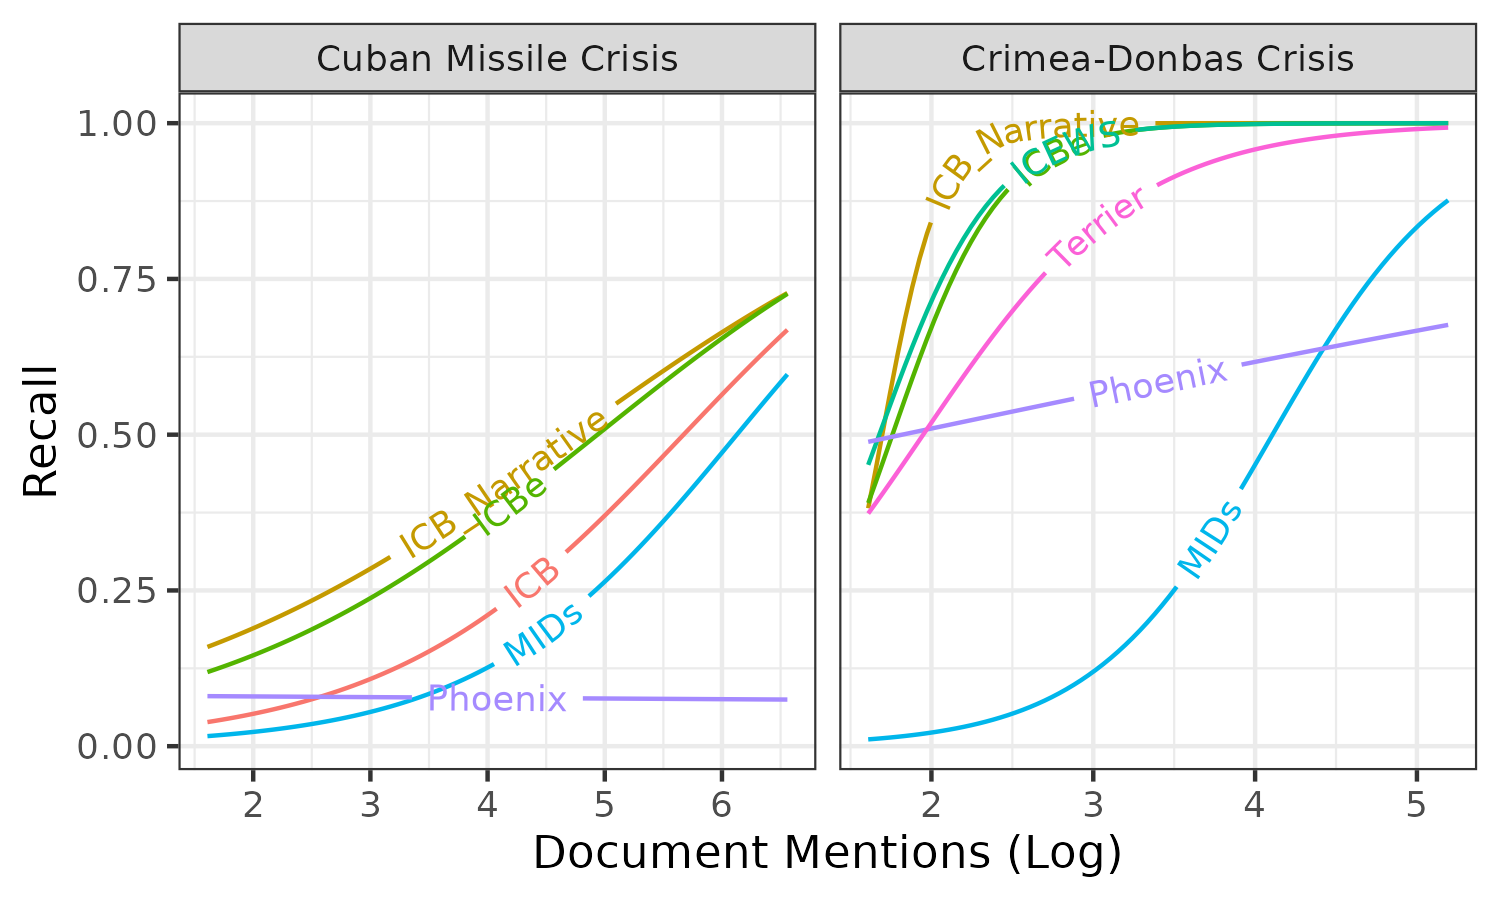
\includegraphics{p_recall.png}
\caption{Recall comparison of two cases across existing state of the art
efforts. Higher y-axis values represent higher recall and higher x-axis
values represent number of times that detail is mentioned across the
full corpus used to construct the synthetic
narrative.}\label{fig-recall-cases}
}
\end{figure}

The second component of event measurement validation is precision. It
does little good to recall a historical event but too vaguely (e.g.~MIDs
describes the Cuban Missile Crisis as a blockade, a show of force, and a
stalemate) or with too much error to be useful for downstream
applications (e.g.~ICEWS records 263 ``Detonate Nuclear Weapons'' events
between 1995-2019). ICBe's ontology and coding system are designed to
strike a balance so that the most important information is recovered
accurately but also abstracted to a level that is still useful and
interpretable.

How does ICBe's precision compare to the existing state of the art? A
researcher should be able to lay out the events of a crisis on a
timeline and read off the macrostructure of an episode from each
individual move. We call this visualization a crisis map, a directed
graph intersected with a timeline. A crisis map using ICBe for the Cuban
Missile Crisis case study is provided in (\textbf{fig-cuba-crisismap?}),
and crisis maps for the two case studies using existing event datasets
can be found in SI Appendix 4.3 and 4.4 and crisis maps for all crises
using all datasets can be found on the companion website. The crisis
maps reveal the episode-level datasets like MIDs or the original ICB are
too sparse and vague to reconstruct the structure of the crisis (SI
Appendix 4.3 and 4.4). On the other end of the spectrum, the high recall
dictionary-based event datasets like Terrier and ICEWs produce so many
noisy events (several hundred thousand) that even with heavy filtering
their crisis maps are completely unintelligible. Further, because of
copyright issues, none of these datasets directly provide the original
text spans making event-level precision difficult to verify.

We further want to verify individual event codings, which we can do in
the case of ICBe because each event is mapped to a specific span of
text. We develop the iconography system for presenting event codings as
coherent statements that can be compared side by side to the original
source narrative for every case on the companion website. We further
provide a stratified sample of event codings alongside their source text
(SI Appendix 4.2). We find both the visualizations of macrostructure and
head-to-head comparisons of ICBe codings to the raw text to strongly
support the quality of ICBe.

(\textbf{fig-umap?}) shows the location of every sentence from the ICBe
corpus in semantic space as embedded using the same large language model
as before, and the median location of each ICBe event tag applied to
those sentences.\footnote{We preprocess sentences to replace named
  entities with a generic Entity token.} Labels reflect the individual
leaves of the ontology and colors reflect the higher level coarse branch
nodes of the ontology. If ICBe has high precision, substantively similar
tags ought to have been applied to substantively similar source text,
which is what we see both in two dimensions in the main plot and via
hierarchical clustering on all dimensions in the dendrogram along the
right-hand side.\footnote{Hierarchical clustering on cosine similarity
  and with Ward's method.}

\begin{figure}
\hypertarget{fig-umap}{%
\centering
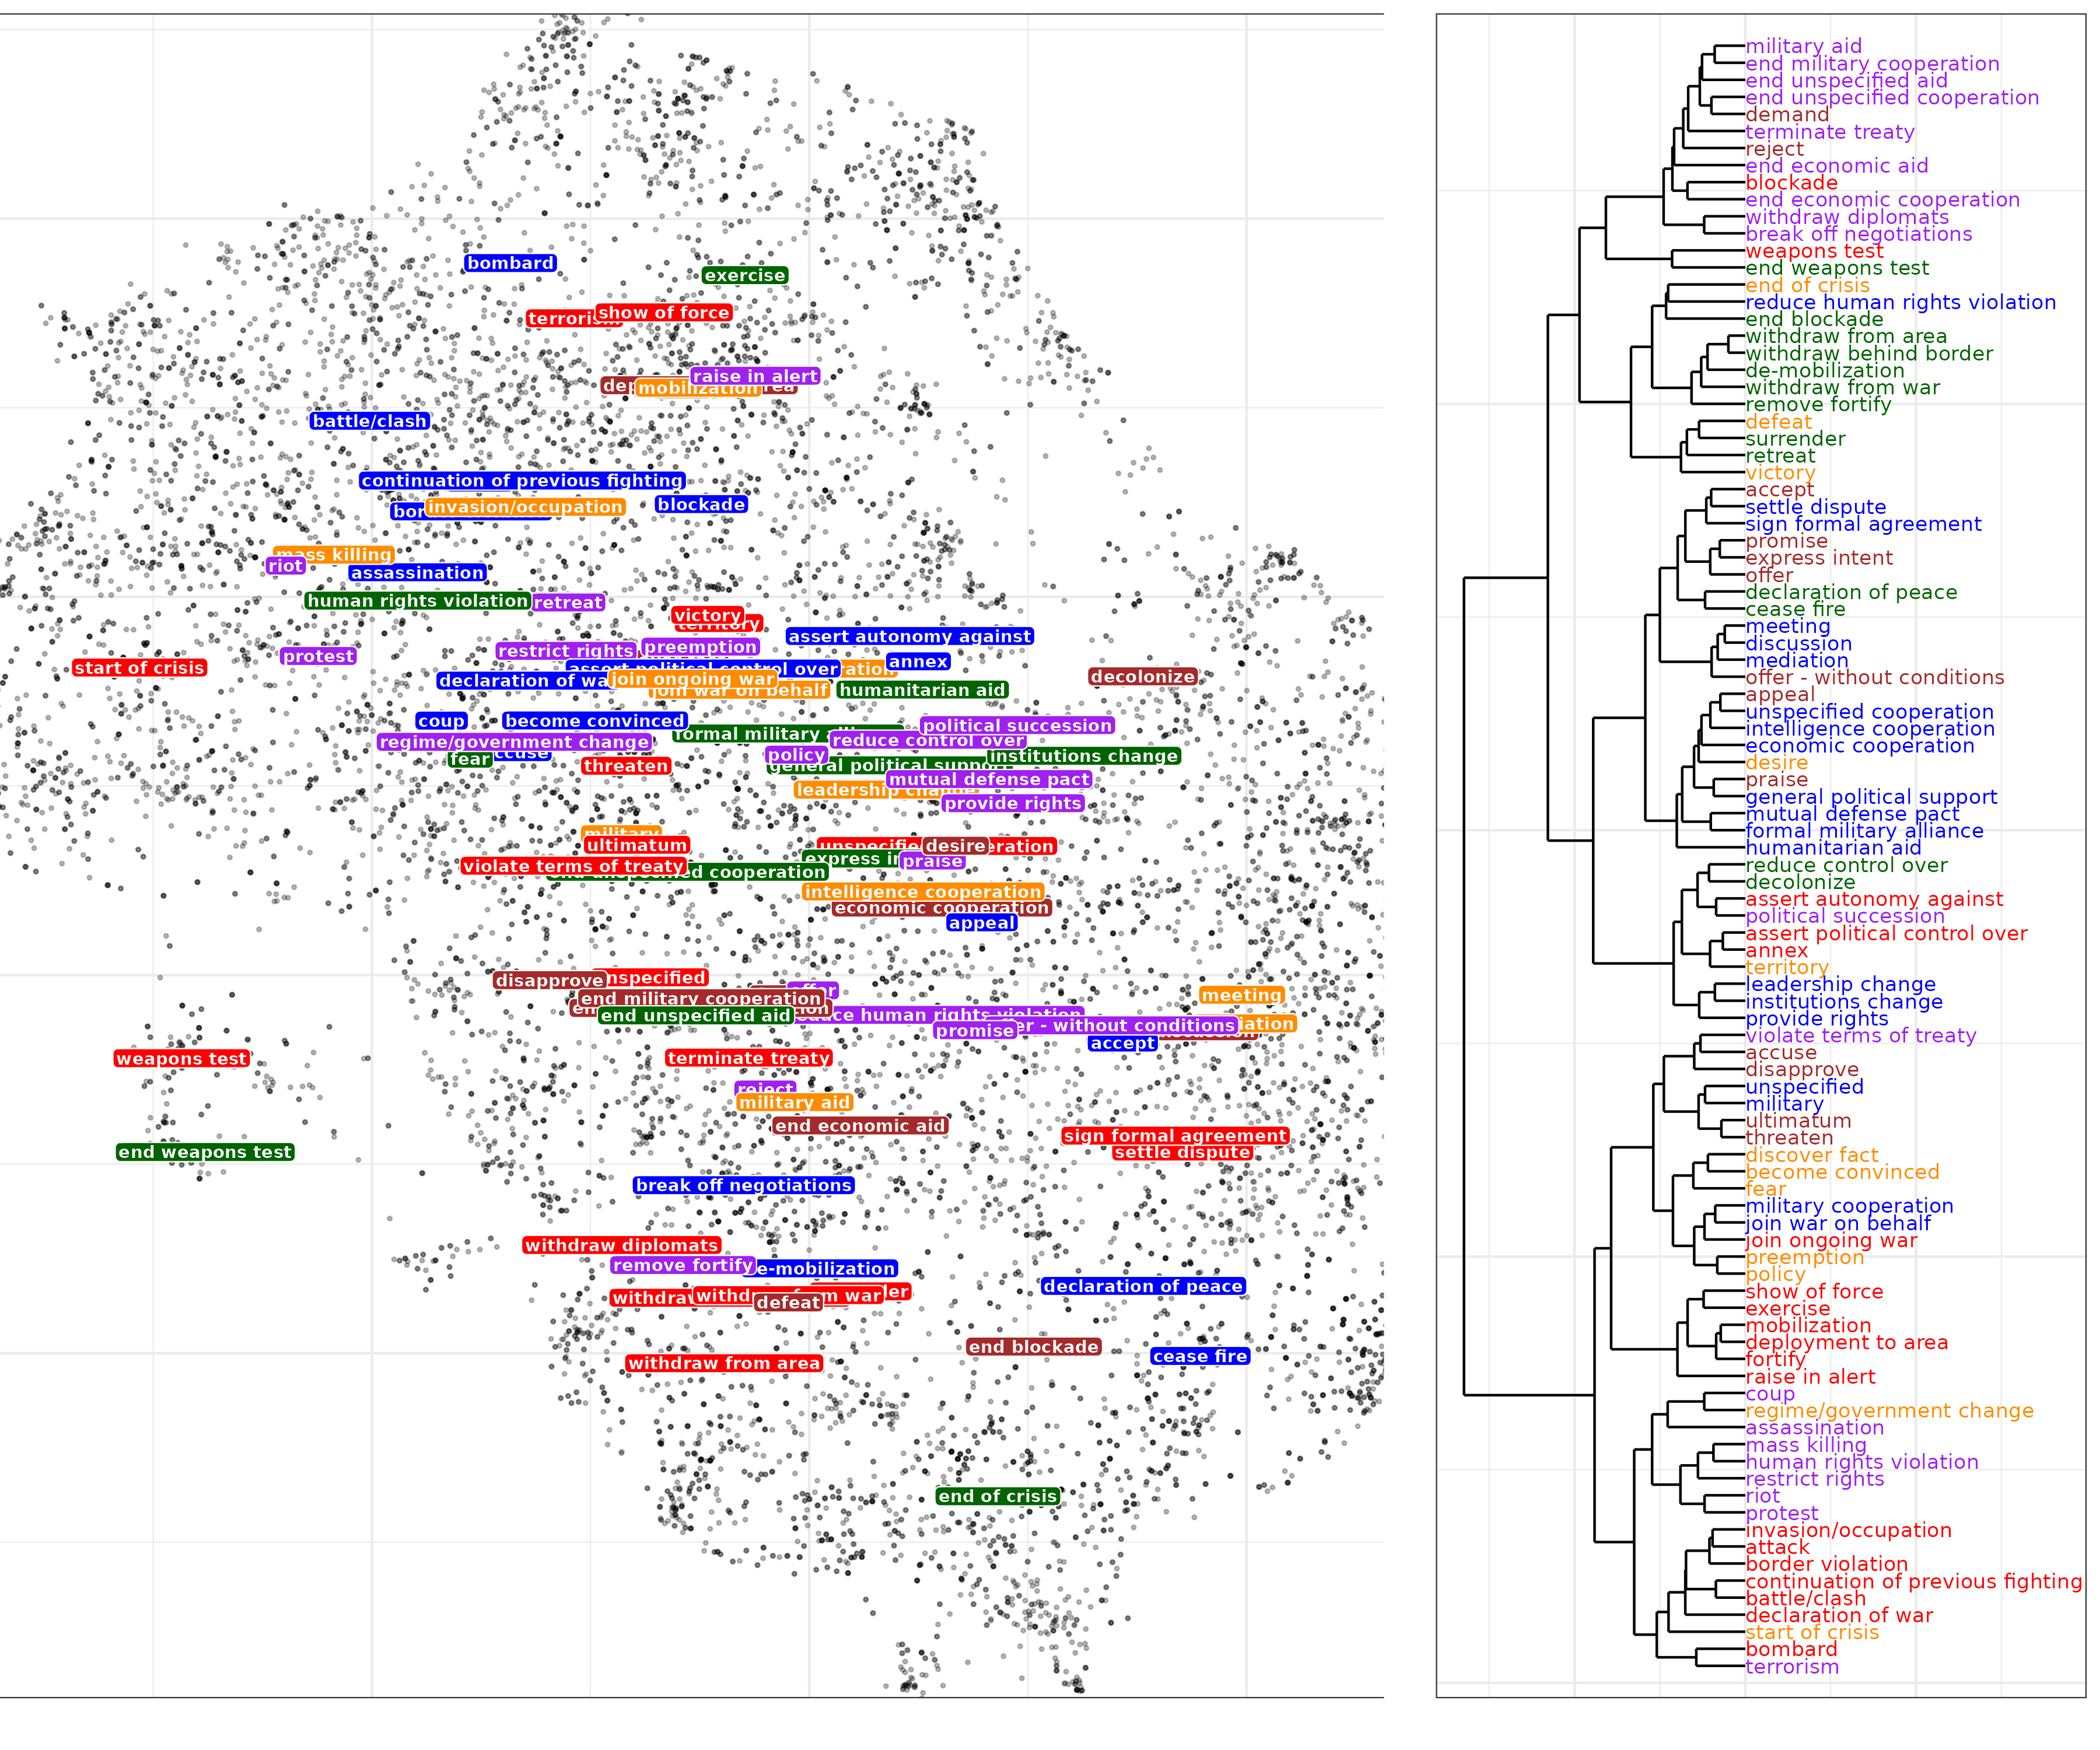
\includegraphics{p_semantic_embeddings_dendro.png}
\caption{Dots represent individual ICB narrative sentences, as embedded
by the Paraphrase-MPNET-base-v2 large language model and flattened into
two dimensions with UMAP. Text labels reflect individual leaves of the
ICBe ontology, and colors represent intermediate branches of the
ontology. Label placement is the median of all of the sentences that the
tag was applied to by the coders. The dendrogram shows hierarchical
clustering of the tags. If ICBe precision is high, then the sentences
that tags were applied to ought to say similar things and the intended
shape of the ontology ought to be visually
recognizable.}\label{fig-umap}
}
\end{figure}

\hypertarget{case-illustrations}{%
\section{Case illustrations}\label{case-illustrations}}

In this section, we focus our validation on two case studies for which
we have produced synthetic narratives using the method described in
Section 3.2. Our proposed measure is a reconstruction task to see
whether our intended ontology can be recovered through only unsupervised
clustering of sentences they were applied to. The first
((\textbf{fig-cuba-narrative?})) is the Cuban Missile Crisis (hereafter
Cuban Missiles) which took place primarily in the second half of 1962,
involved the United States, the Soviet Union, and Cuba, and is widely
known for bringing the world to the brink of nuclear war. The second (SI
Appendix 4.1) is the Crimea-Donbas Crisis (hereafter Crimea-Donbas)
which took place primarily in 2014, involved Russia, Ukraine, and NATO,
and within a decade spiraled into a full-scale invasion. We choose these
cases because they are significant in contemporary international
relations, are widely known across academic disciplines as well as among
the public, and are sufficiently brief to evaluate in depth. They are
similar in that both cases involve a superpower in crisis with a
neighbor that changed from a friendly to a hostile regime, both held
implications for the economic and military security for the superpower
by risking full-scale invasion, and both eventually invited intervention
by an opposing superpower.

\hypertarget{cuban-missile-crisis-1962}{%
\subsection{Cuban Missile Crisis
(1962)}\label{cuban-missile-crisis-1962}}

A synthetic historical narrative for Cuban Missiles appears in
(\textbf{fig-recall-cuba?}), with 51 events drawn from 2,020 documents.
Each row represents a detail that appeared in at least five documents
along with an approximate start date, a handwritten summary, the number
of documents it was mentioned in, and whether it could be identified in
the text of the original ICB corpus, our ICBe events, and any of the
competing existing models.

ICB's improved recall of Cuban Missiles was relative to the state of the
art was summarized in Section 3.2 ((\textbf{fig-recall-cases?})), but
the events that explain that improvement can now be seen. Our ground
truth ICB narrative contains 17/51 of the events from the synthetic
narrative of a case that includes high-level previously classified
details. ICBe captures nearly all details included in ICB as well as
more details from the synthetic narrative than any competing dataset.
Phoenix includes some earlier information than ICBe like the
nationalization of businesses and back channel negotiations, but the
crisis narrative has a clean canonical end with the Soviets agreeing to
withdraw missiles. ICBe stands out in including more communicative
behavior (do -- speech) than existing datasets like US threats to attack
and later promises not to invade. Given the recognized importance of
threat credibility for understanding international conflict, the
addition of this information is a substantively important improvement
over the existing state of the art (Slantchev 2011).

\begin{figure}
\hypertarget{fig-recall-cuba}{%
\centering
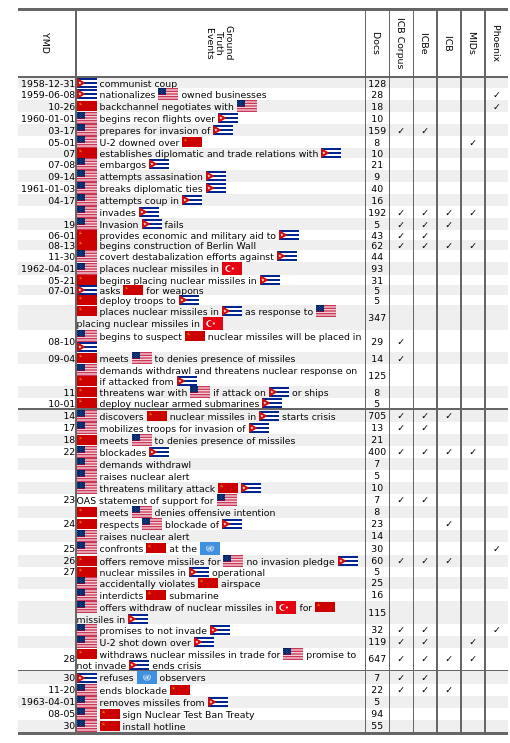
\includegraphics{case_study_cuban_recall.png}
\caption{Synthetic narratives combine several thousand accounts of each
crisis into a single timeline of events, taking only those mentioned in
at least 5 or more documents. Checkmarks represent whether that event
could be hand matched to any detail in the ICB corpus, ICBe dataset, or
any of the other event datasets (SI Appendix 3.2 and
3.3).}\label{fig-recall-cuba}
}
\end{figure}

(\textbf{fig-cuba-crisismap?}) shows the crisis map for the Cuban
Missile Crisis. Looking at the crisis on a timeline, one can now
identify the structure of actors and the environment, along with its
supporting details, in a way that validates the precision of ICBe.
Although harder to measure objectively, this crisis map provides face
valid evidence that ICBe's account is not too vague, but also not
unnecessarily detailed. We include much of the geopolitically important
details like Soviet deployment, US discovery of that deployment,
heightened alert levels, a blockade, and negotiations that ended with a
formal agreement. At the same time, the crisis map indicates that ICBe
does not include unnecessary nuances that preclude useful comparison to
other international events.

\begin{figure}
\hypertarget{fig-cuba-crisismap}{%
\centering
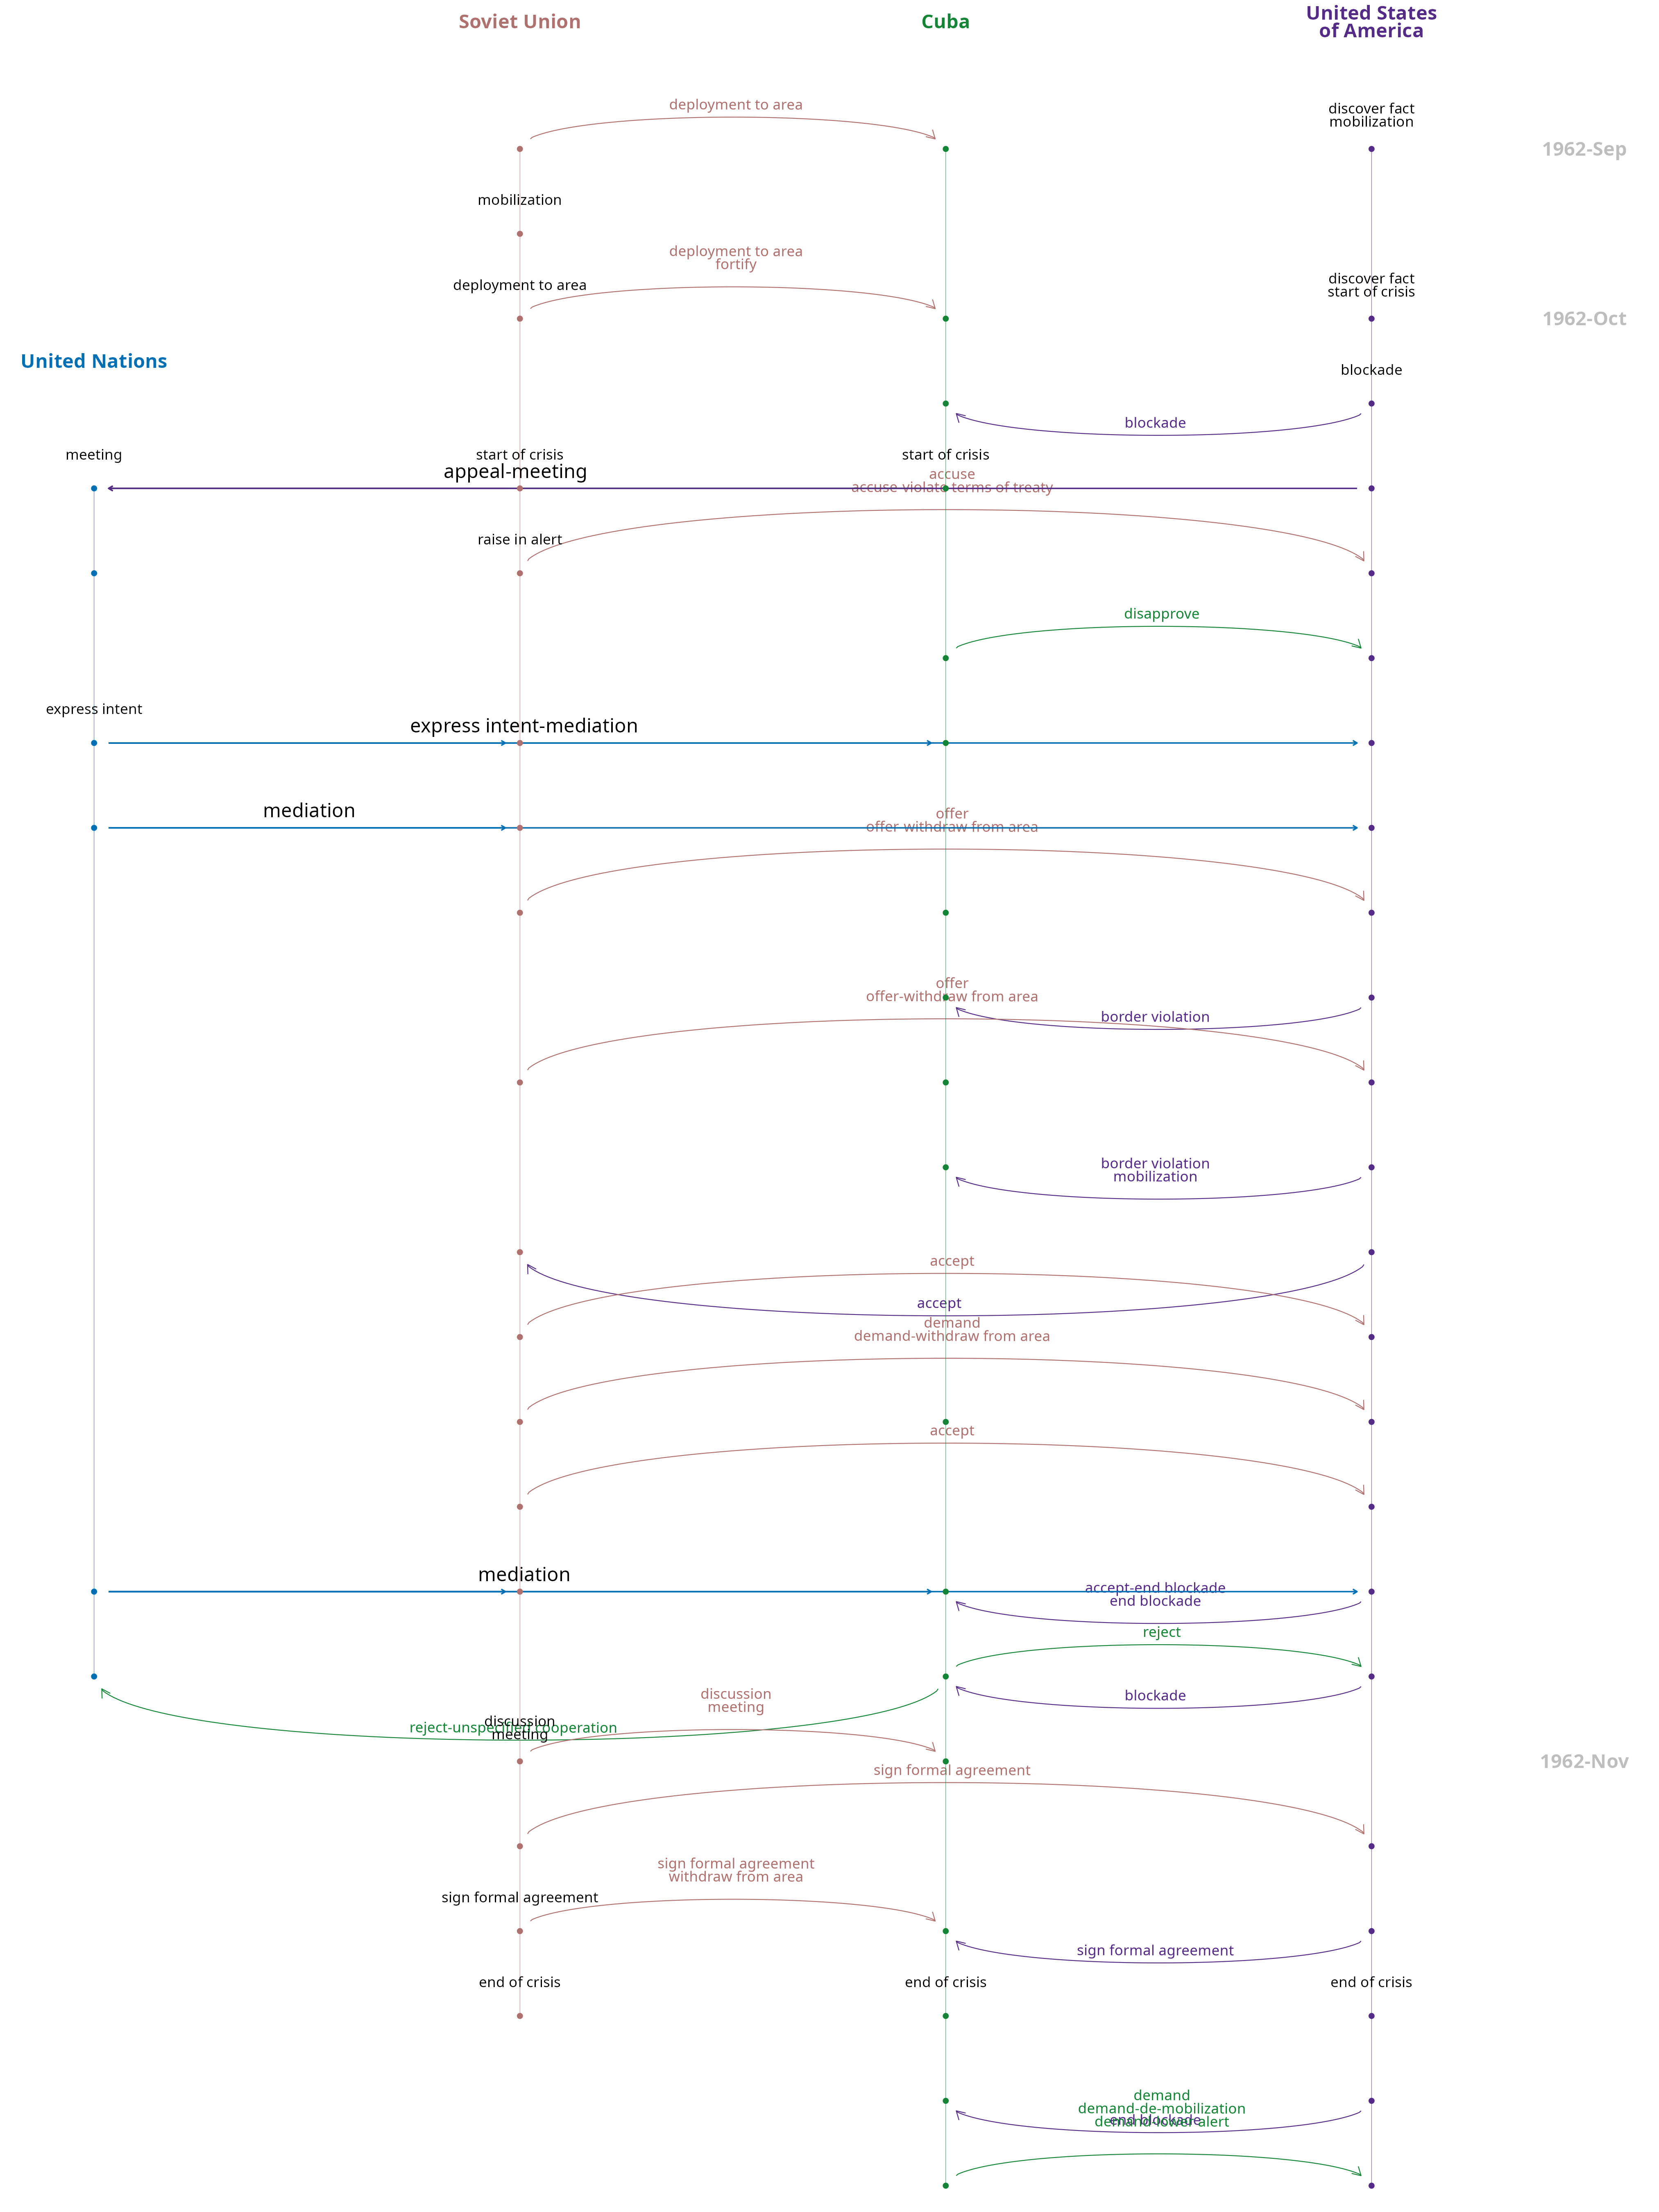
\includegraphics{p_196_icbe.png}
\caption{Crisis map for the Cuban Missile Crisis. The start of the
crisis is at the top and end of the crisis is the bottom, with each
actor in a column with labeled points identifying their speeches,
actions, and thoughts.}\label{fig-cuba-crisismap}
}
\end{figure}

\hypertarget{crimea-donbas-2014}{%
\subsection{Crimea-Donbas (2014)}\label{crimea-donbas-2014}}

A synthetic historical narrative for the 2014 Crimea-Donbas crisis (30
events drawn from 971 documents) appears in
(\textbf{fig-recall-crimea?}). As in the earlier case, rows represent
details that appeared in at least five documents and whether it is
identified in ICBe and existing datasets.

Again quantitatively summarized earlier in Section 3.2
((\textbf{fig-recall-cases?})), our ground truth ICB narrative contains
23/30 of the events from the synthetic narrative. Like the gray zone
precursor to the Cuban Missile crisis
(\textbf{cormacGreyNewBlack2018?}), Ukraine provided several security
guarantees to Russia that were potentially undone, e.g.~a long term
lease on naval facilities in Crimea. But unlike the Cuban Missile
crisis, the end of this crisis is unclear, with the event meekly ending
with a second cease-fire agreement (Minsk II) but continued fighting.
ICBe again recalls more important information about the crisis than any
existing dataset, particularly information concerning the behavior of
non-state separatist groups like the Donetsk People's Republic (DPR) and
Luhansk People's Republic (LPR).

\begin{figure}
\hypertarget{fig-recall-crimea}{%
\centering
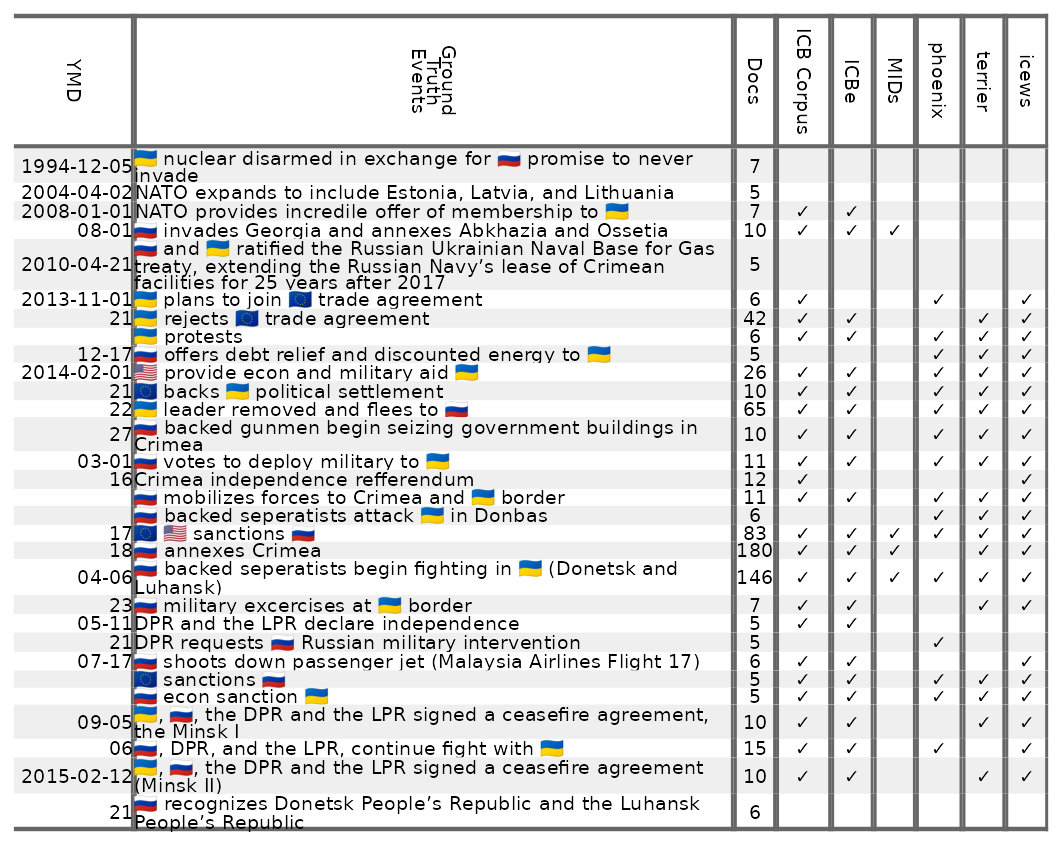
\includegraphics{case_study_crimea_recall.png}
\caption{Synthetic narratives combine several thousand accounts of each
crisis into a single timeline of events, taking only those mentioned in
at least 5 or more documents. Checkmarks represent whether that event
could be hand matched to any detail in the ICB corpus, ICBe dataset, or
any of the other event datasets (SI Appendix 3.2 and
3.3).}\label{fig-recall-crimea}
}
\end{figure}

As this more recent case reflects primarily public reporting rather than
the previously classified details relevant for the Cuban Missile Crisis,
ICBe's improvement relative to the global and real-time coverage of
dictionary-based event systems is still present, but less pronounced. We
want to take seriously the possibility that some functional
transformation could recover the precision of ICBe. For example,
(\textbf{terechshenkoHotCollarLatent2020?}) attempts to correct for the
mechanically increasing amount of news coverage each year by de-trending
violent event counts from Phoenix using a human-coded baseline. Others
have focused on verifying precision for ICEWs on specific subsets of
details against known ground truths, e.g.~geolocation
(\textbf{cookLostAggregationImproving2019?}), protest events (80\%)
(\textbf{wuestExternalValidationProtest2020?}), anti-government protest
networks (46.1\%) (\textbf{jagerLimitsStudyingNetworks2018?}).

We take the same approach here in (\textbf{fig-precision-icews?}),
selecting four specific CAMEO event codings and checking how often they
reflect a true real-world event from the Crimea-Donbas synthetic
narrative. We choose four event types around key moments in the crisis.
The start of the crisis revolves around Ukraine backing out of a trade
deal with the EU in favor of Russia, but ``sign formal agreement''
events act more like a topic detector with dozens of events generated by
discussions of a possible agreement but not the actual agreement which
never materialized. The switch is caught by the ``reject plan, agreement
to settle dispute'', but also continues for Viktor Yanukovych even after
he was removed from power because of articles retroactively discussing
the cause of his removal. Events for ``use conventional military force''
capture a threshold around the start of hostilities and who the
participants were but not any particular battles or campaigns. Likewise,
``impose embargo, boycott, or sanctions'' captures the start of waves of
sanctions and from who but are effectively constant as the news coverage
does not distinguish between subtle changes or additions. In sum,
dictionary-based methods on news corpora tend to have high recall
because they parse everything in the news, but for the same reason,
their specificity for most event types is too low to back out individual
chess-like sequencing that ICBe aims to record.

\begin{figure}
\hypertarget{fig-precision-icews}{%
\centering
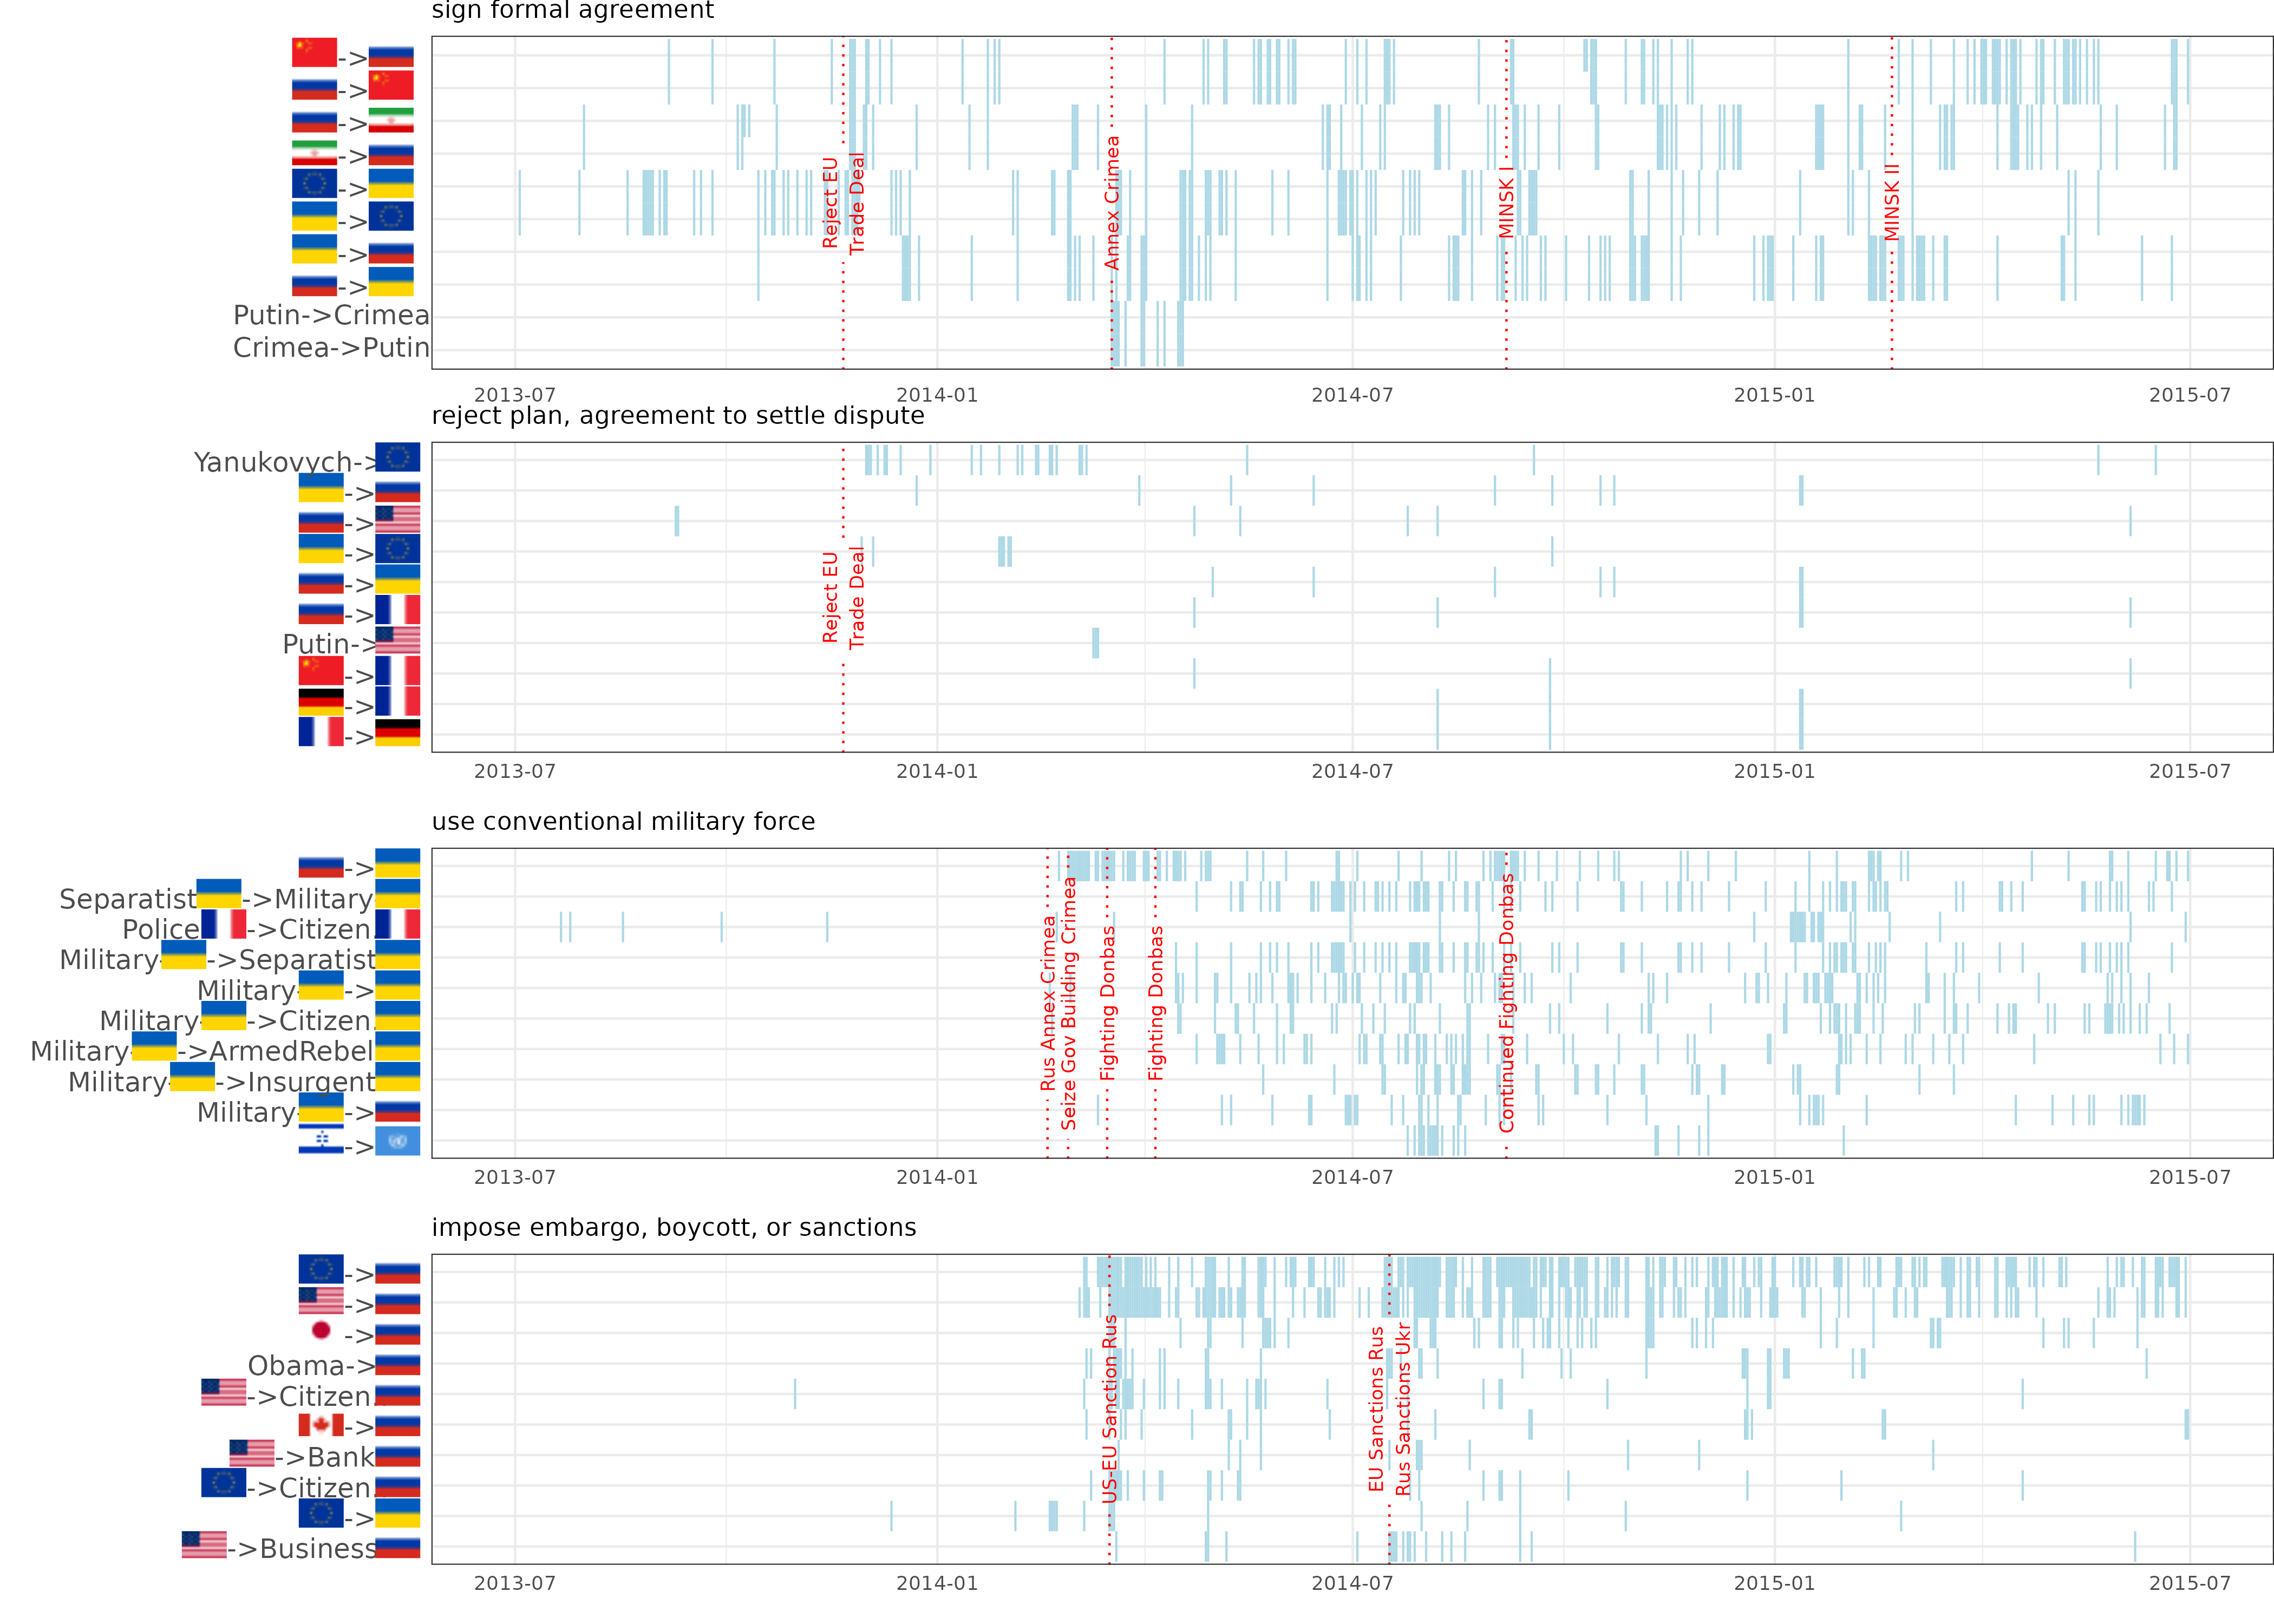
\includegraphics{p_precision_icews.png}
\caption{The unit of analysis is the dyad-day. Top 10 most active dyads
per category shown. Red text shows events from the synthetic narrative
relative to that event category. Blue bars indicate an event recorded by
ICEWs for that dyad on that day.}\label{fig-precision-icews}
}
\end{figure}

\hypertarget{conclusion}{%
\section{Conclusion}\label{conclusion}}

We investigated event abstraction from narratives describing key
historical episodes in international relations. We synthesized a prior
belief about the latent unobserved phenomena that drive these events in
international relations and proposed a mapping to observable concepts
that enter into the observed historical record. We designed an ontology
with high coverage over those concepts and developed a training
procedure and technical stack for human coding of historical texts.
Multiple validity checks find the resulting codings have high internal
validity (e.g.~intercoder agreement) and external validity
(i.e.~matching source material in both micro-details at the sentence
level and macro-details spanning full historical episodes). Further,
these codings perform much better in terms of recall, precision,
coverage, and overall coherence in capturing these historical episodes
than existing event systems used in international relations.

We release several open-source products along with supporting code and
documentation to further advance the study of international relations,
event extraction, and natural language processing. The first is the
International Crisis Behavior Events (ICBe) dataset, an event-level
aggregation of what took place during the crises identified by the ICB
project. These data are appropriate for statistical analysis of hard
questions about the sequencing of events (e.g.~escalation and
de-escalation of conflicts).\footnote{Using ICBe data
  (\textbf{gannonOneIfLand2022?}) finds that cross-domain crises are
  shorter and less violent than same-domain crises.} Second, we provide
a coder-level disaggregation with multiple codings of each sentence by
experts and undergrads that allows for the introduction of uncertainty
and human interpretation of events. Further, we release a direct mapping
from the codings to the source text at the sentence level as a new
resource for natural language processing. Finally, we provide a
companion website that incorporates detailed visualizations of all of
the data introduced here at crisisevents.org.

\hypertarget{funding}{%
\section{Funding}\label{funding}}

This work was supported by a grant from the Office of Naval Research
\[N00014-19-1-2491\] and from the Charles Koch Foundation \[20180481\].
The financial sponsors played no in the design, execution, analysis and
interpretation of data, or writing of the study.

\hypertarget{acknowledgements}{%
\section{Acknowledgements}\label{acknowledgements}}

We thank the ICB Project and its directors and contributors for their
foundational work and their help with this effort. We make special
acknowledgement of Michael Brecher for helping found the ICB project in
1975, creating a resource that continues to spark new insights to this
day. We thank the many undergraduate coders. Thanks to the Center for
Peace and Security Studies and its membership for comments. Special
thanks to Rebecca Cordell, Philip Schrodt, Zachary Steinert-Threlkeld,
and Zhanna Terechshenko for their generous feedback. Thank you to the
cPASS research assistants: Helen Chung, Daman Heer, Syeda ShahBano Ijaz,
Anthony Limon, Erin Ling, Ari Michelson, Prithviraj Pahwa, Gianna Pedro,
Tobias Stodiek, Yiyi `Effie' Sun, Erin Werner, Lisa Yen, and Ruixuan
Zhang.

\hypertarget{author-contributions}{%
\section{Author Contributions}\label{author-contributions}}

Conceptualization: R.W.D., E.G., J.L.; Methodology: R.W.D., T.L.S.;
Software: R.W.D.; Validation: R.W.D., T.L.S.; Formal Analysis: R.W.D.,
T.L.S.; Investigation: S.C., R.W.D., J.A.G., C.K., N.L., E.M., J.M.C.N.,
D.P., D.Q., J.W.; Data Curation: R.W.D., D.Q., T.L.S., J.W.; Writing -
Original Draft: R.W.D., T.L.S.; Writing - Review \& Editing: R.W.D.,
J.A.G., E.G., T.L.S.; Visualization: R.W.D., T.L.S.; Supervision: E.G.;
Project Administration: S.C., R.W.D., J.A.G., D.Q., T.L.S., J.W.;
Funding Acquisition: E.G., J.L.

\hypertarget{data-availability-statement}{%
\section{Data Availability
Statement}\label{data-availability-statement}}

This article's data, supplementary appendix, replication material, and
visualizations of every historical episode are available on the GitHub
repository
\href{https://urldefense.com/v3/__https://github.com/CenterForPeaceAndSecurityStudies/ICBEventData__;!!Mih3wA!WxDJtEczKfxGTh0S2Krunap8ReymFEL5iTWaSfOHeqlSdyfRx77zmjBSWO1OAm13$}{ICBEventData}
and through the companion website crisisevents.org.

\hypertarget{competing-interests-declaration}{%
\section{Competing Interests
Declaration}\label{competing-interests-declaration}}

The authors declare that there are no competing interests.

\clearpage

\hypertarget{works-cited}{%
\section*{Works Cited}\label{works-cited}}
\addcontentsline{toc}{section}{Works Cited}

\hypertarget{refs}{}
\begin{CSLReferences}{1}{0}
\leavevmode\vadjust pre{\hypertarget{ref-benyehudaEthnicActorsInternational2006}{}}%
Ben-Yehuda, Hemda, and Meirav Mishali--Ram. 2006. {``Ethnic {Actors} and
{International} {Crises}: {Theory} and {Findings}, 1918--2001.''}
\emph{International Interactions} 32 (1): 49--78.
\url{https://doi.org/10.1080/03050620600584435}.

\leavevmode\vadjust pre{\hypertarget{ref-brecher_study_1997}{}}%
Brecher, Michael, and Jonathan Wilkenfeld. 1997. \emph{A {Study} of
{Crisis}}. University of Michigan Press.

\leavevmode\vadjust pre{\hypertarget{ref-gannon_shadowdeterrencewhy_2023}{}}%
Gannon, J Andrés, Erik Gartzke, Jon R. Lindsay, and Peter Schram. 2023.
{``The {Shadow} of {Deterrence}: {Why Capable Actors Engage} in
{Contests Short} of {War}.''} \emph{Journal of Conflict Resolution},
April. \url{https://doi.org/10.1177/00220027231166345}.

\leavevmode\vadjust pre{\hypertarget{ref-slantchev_militarythreatscosts_2011}{}}%
Slantchev, Branislav L. 2011. \emph{Military Threats: The Costs of
Coercion and the Price of Peace}. Cambridge ; New York: Cambridge
University Press.

\leavevmode\vadjust pre{\hypertarget{ref-turberville_historyobjectivesubjective_1933}{}}%
Turberville, A. S. 1933. {``History {Objective} and {Subjective}.''}
\emph{History} 17 (68): 289--302.
\url{https://www.jstor.org/stable/24400365}.

\end{CSLReferences}

\bibliographystyle{unsrt}
\bibliography{paper.bib}


\end{document}
